%% LyX 1.4.3 created this file.  For more info, see http://www.lyx.org/.
%% Do not edit unless you really know what you are doing.
\documentclass[english]{book}
\usepackage[T1]{fontenc}
\usepackage[latin1]{inputenc}
\usepackage{geometry}
\geometry{verbose,letterpaper,tmargin=1in,bmargin=1in,lmargin=1in,rmargin=1in}
\pagestyle{plain}
\setcounter{secnumdepth}{3}
\setcounter{tocdepth}{3}
\usepackage{array}
\usepackage{float}
\usepackage{color}
\usepackage{graphicx}
\IfFileExists{url.sty}{\usepackage{url}}
                      {\newcommand{\url}{\texttt}}

\makeatletter

%%%%%%%%%%%%%%%%%%%%%%%%%%%%%% LyX specific LaTeX commands.
\newcommand{\noun}[1]{\textsc{#1}}
%% Bold symbol macro for standard LaTeX users
\providecommand{\boldsymbol}[1]{\mbox{\boldmath $#1$}}

%% Because html converters don't know tabularnewline
\providecommand{\tabularnewline}{\\}

%%%%%%%%%%%%%%%%%%%%%%%%%%%%%% Textclass specific LaTeX commands.
\newenvironment{lyxcode}
{\begin{list}{}{
\setlength{\rightmargin}{\leftmargin}
\setlength{\listparindent}{0pt}% needed for AMS classes
\raggedright
\setlength{\itemsep}{0pt}
\setlength{\parsep}{0pt}
\normalfont\ttfamily}%
 \item[]}
{\end{list}}

%%%%%%%%%%%%%%%%%%%%%%%%%%%%%% User specified LaTeX commands.
\usepackage{hyperref}

\usepackage{babel}
\makeatother
\begin{document}
%
\begin{figure}[H]
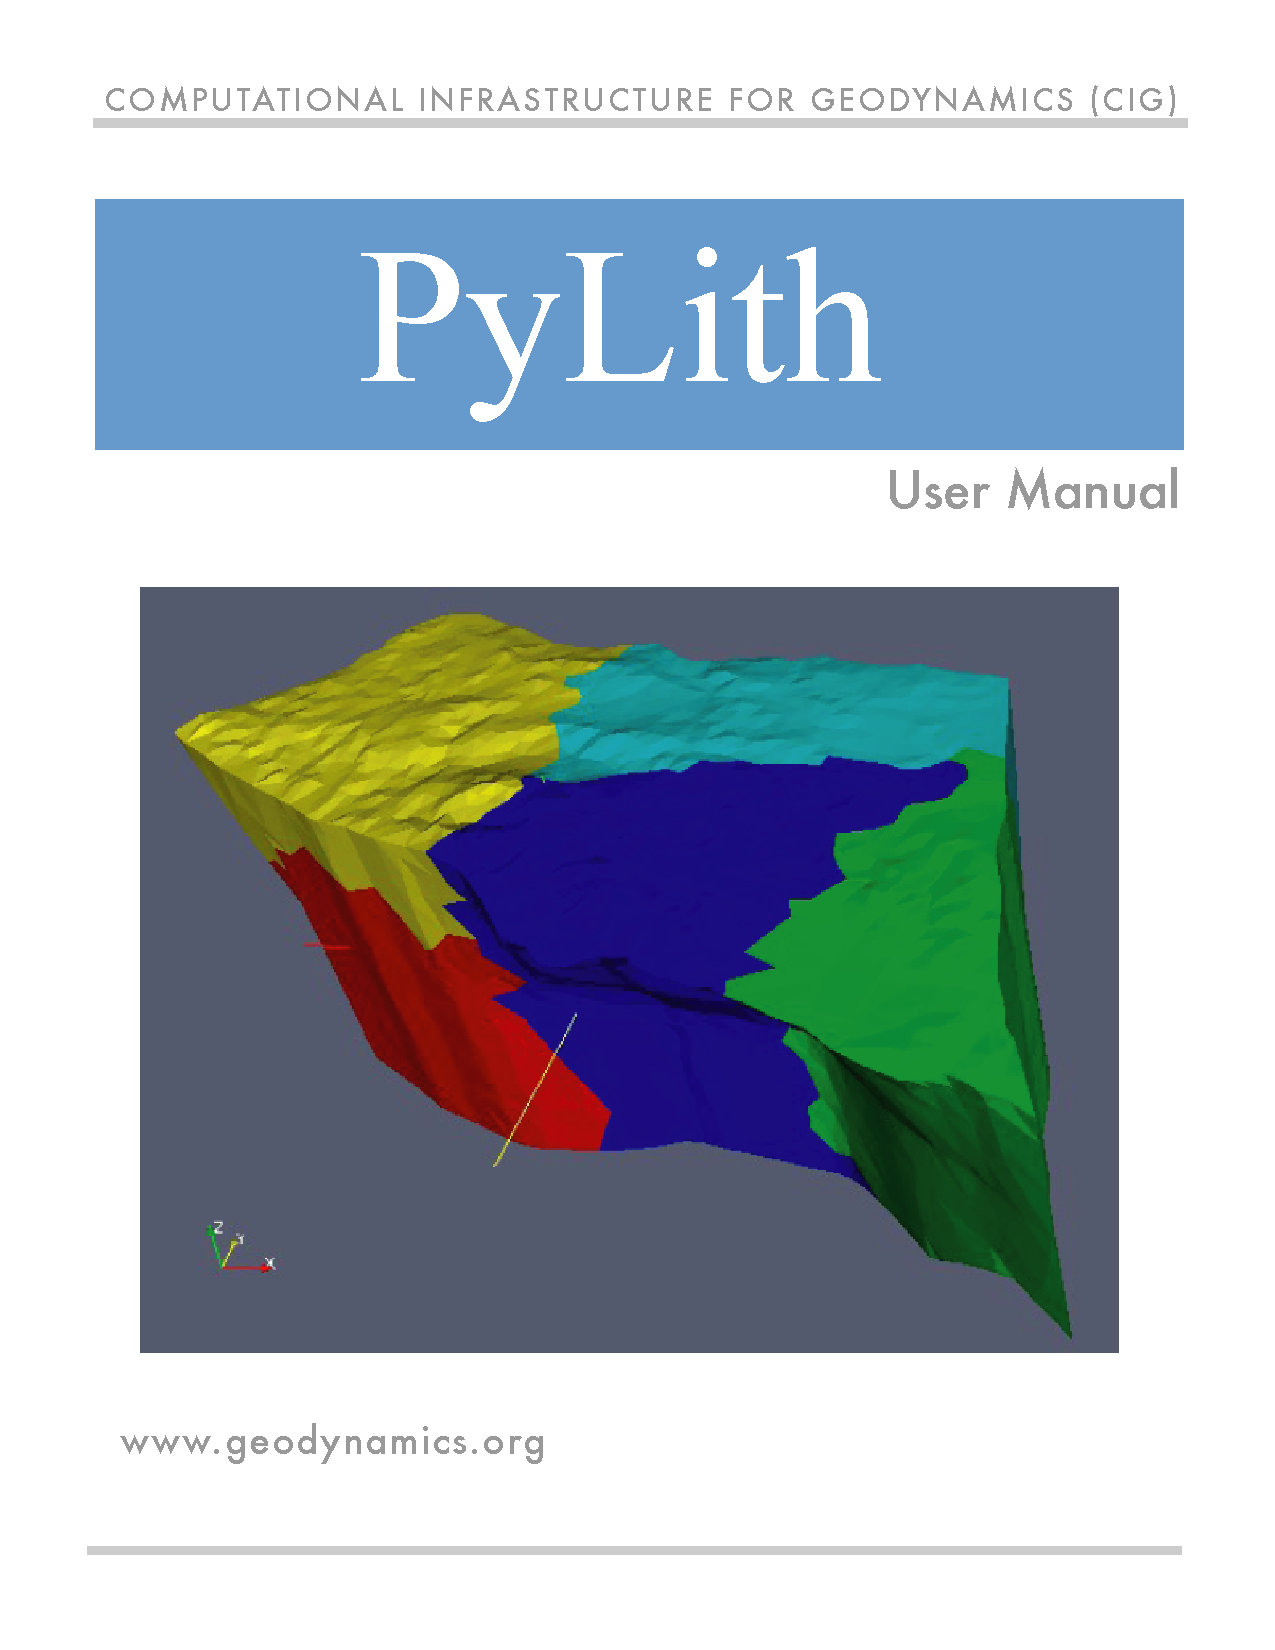
\includegraphics[width=0.75\paperwidth]{pylith_cover}
\end{figure}


\thispagestyle{empty}


\frontmatter

\tableofcontents{}

\listoffigures



\chapter{Preface}


\section{About This Document}

This document is organized into two parts. The first part begins with
an introduction to PyLith and discusses the types of problems that
PyLith can solve and how to run the software; the second part provides
appendices and references.


\section{Who Will Use This Documentation}

This documentation is aimed at two categories of users: scientists
who prefer to use prepackaged and specialized analysis tools, and
experienced computational Earth scientists. Of the latter, there are
likely to be two classes of users: those who just run models, and
those who modify the source code. Users who modify the source are
likely to have familiarity with scripting, software installation,
and programming, but are not necessarily professional programmers.

\section{Conventions}

\warning{This is a warning.}
\important{This is something important.}
\tip{This is a tip, helpful hint, or suggestion.}

For features recently added to PyLith, we show the version number when
they were added.\newfeature{v2.1.4}

\subsection{Command Line Arguments}

Exmaple of a command line argument: \commandline{-{}-help}.

\subsection{Filenames and Directories}

Example of filenames and directories: \filename{pylith}, \filename{/usr/local}.

\subsection{Unix Shell Commands}

Commands entered into a Unix shell (i.e., terminal) are shown in a
box. Comments are delimited by the \# character. We use 
{\tt \$\$} to indicate the bash shell prompt.
\begin{shell}
# This is a comment.
$$ ls -l
\end{shell}

\subsection{Excerpts of cfg Files}

Example of an excerpt from a \filename{.cfg} file:
\begin{cfg}
# This is a comment.
<h>[pylithapp.problem]</h>
<p>timestep</p> = 2.0*s ; Time step comment.
<f>bc</f> = [x_pos, x_neg]
\end{cfg}

\section{Citation}

The Computational Infrastructure for Geodynamics (CIG) (\url{geodynamics.org})
is making this source code available to you at no cost in hopes that
the software will enhance your research in geophysics. A number of
individuals have contributed a significant portion of their careers
toward the development of this software. It is essential that you
recognize these individuals in the normal scientific practice by citing
the appropriate peer-reviewed papers and making appropriate acknowledgments
in talks and publications. The preferred way to generate the list
of publications (in Bib\TeX{} format) to cite is to run your simulations
with the \commandline{-{}-include-citations} command line argument, or
equivalently, the \commandline{-{}-petsc.citations} command line argument.
The \commandline{-{}-help-citations} command line argument will generate
the Bib\TeX{} entries for the references mentioned below.

The following peer-reviewed paper discussed the development of PyLith:
\begin{itemize}
\item Aagaard, B. T., M. G. Knepley, and C. A. Williams (2013). A domain
decomposition approach to implementing fault slip in finite-element
models of quasi-static and dynamic crustal deformation, \textit{Journal
of Geophysical Research: Solid Earth}, 118, doi: 10.1002/jgrb.50217.
\end{itemize}
To cite this manual, use:
\begin{itemize}
\item Aagaard, B., M. Knepley, C. Williams (2016), \emph{PyLith User Manual,
Version 2.1.4.} Davis, CA: Computational Infrastructure of Geodynamics.\\
URL: geodynamics.org/cig/software/pylith/pylith\_manual-2.1.4.pdf
\end{itemize}

\section{Support}

Current PyLith development is supported by the CIG, and internal GNS
Science \url{www.gns.cri.nz} and U.S. Geological Survey \url{www.usgs.gov}
funding. Pyre development was funded by the Department of Energy's
\url{www.doe.gov/engine/content.do} Advanced Simulation and Computing
program and the National Science Foundation's Information Technology
Research (ITR) program.

This material is based upon work supported by the National Science
Foundation under Grants No. 0313238, 0745391, and EAR-0949446. Any
opinions, findings, and conclusions or recommendations expressed in
this material are those of the author(s) and do not necessarily reflect
the views of the National Science Foundation.


\section{Acknowledgments}

Many members of the community contribute to PyLith through reporting
bugs, suggesting new features and improvements, running benchmarks,
and asking questions about the software. In particular, we thank Surendra
Somala for contributing to the development of the fault friction implementation.


\section{Request for Comments}

Your suggestions and corrections can only improve this documentation.
Please report any errors, inaccuracies, or typos to the CIG Short-Term
Tectonics email list \url{cig-short@geodynamics.org}. 


\mainmatter

\chapter{Introduction}

\section{Overview}

PyLith is a multi-scale simulation software package for earthquake
physics. It is portable, scalable software for simulation of crustal
deformation across spatial scales ranging from meters to hundreds of
kilometers and temporal scales ranging from milliseconds to thousands
of years

\section{History}

This first version of PyLith is a direct descendant of Lithomop and
marks the first version that runs in parallel. Lithomop was the
product of major reengineering of Tecton, a finite-element code for
simulating static and quasi-static crustal deformation. The major new
features present in Lithomop included dynamic memory allocation and
the use of the Pyre simulation framework and PETSc solvers. </para>
<para> PyLith is currently being rewritten from scratch to create a
much more modular, powerful simulation package. This new code will
include earthquake dynamics (both rupture propagation and seismic wave
propagation). A beta release is expected in late 2006.

\section{Governing Equations}

Both LithoMop3d and PyLith-0.8 are quasi-static codes, meaning that
time-dependence only enters through the constitutive relationships and
the loading conditions. The description here is for the small-strain
formulation, which is the only formulation available at present. If a
large deformation solution is desired, interested users may contact
Charles Williams (willic3@rpi.edu) about a version of the finite
element code TECTON.

The problem is formulated in terms of the stresses ($\sigma_{ij}$),
displacements ($u_i$), and body forces per unit volume
(figs/g-inlineeq1.eps). We use standard index notation for all
equations here, such that repeated indices imply summation and a comma
denotes differentiation. For a general three-dimensional body, the
problem must satisfy the equilibrium conditions
\begin{equation}
  \text{figs/g-eq1.eps}
\end{equation}
subject to the natural boundary conditions
\begin{equation}
  \text{figs/g-eq2.eps}
\end{equation}
and the essential boundary conditions
\begin{equation}
  \text{figs/g-eq3.eps}
\end{equation}
The surface of the body is $S$, given by
\begin{equation}
  \text{figs/g-eq4.eps}
\end{equation}
The $n_j$ are the components of the unit normal vector to $S$, the
\begin{equation}
  \text{figs/g-inlineeq2.eps}
\end{equation}
are the components of the surface tractions, and the 
\begin{equation}
  \text{figs/g-inlineeq3.eps}
\end{equation}
are the components of the applied displacements. The stresses are
computed from the strains and any existing initial stresses using a
given constitutive relationship. The strains are given by
\begin{equation}
\text{figs/g-eq5.eps}  
\end{equation}
For a linear elastic material, the constitutive relationship between
stress and strain is
\begin{equation}
  \text{figs/g-eq6.eps}
\end{equation}
where
\begin{equation}
  \text{figs/g-inlineeq4.eps}
\end{equation}
are the initial stresses, and $C$
\begin{equation}
  \text{g-inlineeq5.eps}
\end{equation}
is the elastic constitutive relation.

For inelastic behavior (viscous, plastic, etc.), we assume an additive
decomposition of the strain tensor into elastic and inelastic parts,
and use an integrated form of the classical incremental theory of
plasticity. At time $t+\Delta t$, he stresses are therefore computed
from the total elastic strain:
\begin{equation}
  \text{figs/g-eq7.eps}
\end{equation}
where
\begin{equation}
  \text{figs/g-inlineeq6.eps}
\end{equation}
are the total strains and
\begin{equation}
  \text{figs/g-inlineeq7.eps}
\end{equation}
are the inelastic strains, with the difference being the elastic
strains. In our actual computations, we use a formulation that
decomposes the stresses into the deviatoric and volumetric parts,
using ideas based on the "effective stress function"
\cite{Kojic:Bathe:1987}. This allows the time integration of stresses
to be performed in terms of a single parameter related to the second
deviatoric stress invariant.

\section{Software Components}

PyLith is separated into modules to encapsulate behavior and
facilitate use across multiple applications. That way expert users can
replace functionality of a wide variety of components without
recompiling or polluting the main code. External packages reduce
development time and enhance computational efficiency, for example,
PyLith runs 2x faster by using the PETSc linear solver.

PyLith is based on several programming languages. High-level code is
written in Python; this rich, expressive interpreted language with
dynamic typing reduces development time. Low-level code is written in
Fortran 77 for fast execution. Bindings, written in C/C++, are used to
allow the low-level code (Fortran 77) to be called from high-level
code (Python).

PyLith makes extensive use of external software. Pyre is a science
neutral simulation framework being developed at Caltech. PETSc is used
to perform operations on matrices and vectors in parallel.

\subsection{PETSc}

\href{http://www-unix.mcs.anl.gov/petsc/petsc-as/}{PETSc}, the
Portable, Extensible Toolkit for Scientific computation, provides a
suite of routines for parallel, numerical solution of partial
differential equations for linear and nonlinear systems with large,
sparse systems of equations. PETSc includes solvers that implement a
variety of Newton and Krylov subspace methods. It can also interface
with many external packages, including BlockSolve95, ESSL, Matlab,
ParMeTis, PVODE, and SPAI, thereby providing additional solvers and
interaction with other software packages.

PETSc includes interfaces for Fortran, C, and C++ for nearly all of
the routines and PETSc can be installed on most Unix systems. PETSc
can be built with user supplied highly optimized linear algebra
routines (e.g., ATLAS and commercial versions of BLAS/LAPACK), thereby
improving application performance. Users can use PETSc parallel
matrices, vectors, and other data structures for most parallel
operations, eliminating the need for explicit calls to Message Passing
Interface (MPI) routines. Many settings and options can be controlled
with PETSc specific command-line arguments, including selection of
preconditions, solvers, and generation of performance logs.

\subsection{Pyre}

Pyre is an object-oriented environment capable of specifying and
launching numerical simulations on multiple platforms, including
Beowulf class parallel computers and grid computing systems. Pyre
allows the binding of multiple components such as solid and fluid
models used in Earth science simulations, and different meshers. The
Pyre framework enables the elegant setup, modification and launching
of massively parallel three-dimensional solver applications.

Pyre is a framework, a combination of software and design philosophy
that promotes the reuse of code. In their canonical software design
book, {\em Design Patterns}, Erich Gamma {\it et al}.  condense the
concept of a framework concept down to, "When you use a framework, you
reuse the main body and write the code it calls." In the context of
frameworks and object-oriented programming, Pyre can be thought of as
a collection of classes and the way their instances interact.
Programming applications based on Pyre will look similar to those
written in any other object-oriented language. The Pyre framework
contains a subset of parts that make up the overall framework. Each of
those parts is designed to solve a specific problem.

The framework approach to computation offers many advantages. It
permits the exchange of codes and promotes the reuse of standardized
software while preserving efficiency. Frameworks are also an efficient
way to handle changes in computer architecture. They present
programmers and scientists with a unified and well-defined task and
allow for shared costs of the housekeeping aspects of software
development. They provide greater institutional continuity to model
development than piecemeal approaches.


The Pyre framework incorporates features aimed at enabling the
scientific non-expert to perform tasks easily without hindering the
expert. Target features for end users allow complete and intuitive
simulation specification, reasonable defaults, consistency checks of
input, good diagnostics, easy access to remote facilities, and status
monitoring. Target features for developers include easy access to user
input, a shorter development cycle, and good debugging support.

\begin{figure}[htbp]
  \begin{center}
    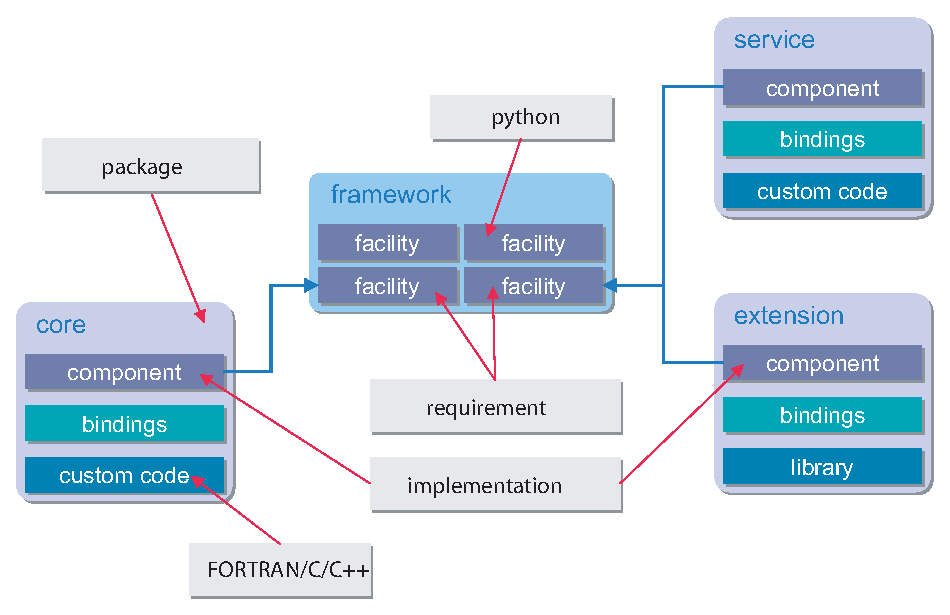
\includegraphics[scale=0.75]{figs/pyre_overview}
    \caption{Pyre Architecture. The integration framework is a set of
      cooperating abstract services.}
  \end{center}
\end{figure}

\section{PyLith Design}

In transforming Lithomop, a serial code, into PyLith, a parallel code,
a principal concern was to preserve the existing structure of the
serial Fortran code. Active development of purely analytic features in
PyLith, such as new material models or discretization schemes, depends
on the familiarity of application scientists with the traditional
Fortran programming paradigm. Global, topological operation should be
strictly segregated from the existing code. In fact, with the
exception of integrating PETSc for serial linear algebra and solver
operations, PyLith can be run purely in serial without activating any
of the parallel capabilities.

In order to accomplish this separation, we use the PETSc
\classname{Sieve} structure to create a model of the serial
PyLith mesh. This model is then partitioned and distributed to a set
of processes. Each process receives a self-consistent mesh, meaning
the pieces are overlapping. Each process then executes a serial PyLith
step on that particular mesh piece. The PETSc linear algebra
operations are overloaded, using the \classname{Sieve}
information, to produce a globally consistent field.

 
\chapter{\label{cha:Installation-and-Getting}Installation and Getting Help}

Installation of PyLith on a desktop or laptop machine is, in most
cases, very easy. Binary packages have been created for Linux and
Mac OS X platforms. You can also run PyLith inside a Docker container,
which provides a virtual Linux environment on any platform that Docker
supports, including Linux, Mac OS X, and Windows. Installation of
PyLith on other operating systems -- or installation on a cluster
-- requires building the software from the source code, which can
be difficult for inexperienced users. We have created a small utility
called PyLith Installer that makes installing PyLith and all of its
dependencies from source much easier. Help is available from both
a CIG mailing list and the Github issue tracking system \url{https://github.com/geodynamics/pylith/issues}.


\section{\label{sec:Getting-Help-and}Getting Help and Reporting Bugs}

The CIG Short-Term Crustal Dynamics Mailing List \url{cig-short@geodynamics.org}
is dedicated to CIG issues associated with short-term crustal dynamics,
including the use of PyLith. You can subscribe to the mailing list
and view messages at cig-short Mailing List \url{geodynamics.org/cig/lists/cig-short}. 

CIG uses \texttt{Github} for source control and bug tracking. If you
find a bug in PyLith, please submit a bug report to the Github issue
tracking system for PyLith \url{https://github.com/geodynamics/pylith/issues}.
Of course, it is helpful to first check to see if someone else already
submitted a report related to the issue; one of the CIG developers
may have posted a work around to the problem. You can reply to a current
issue by clicking on the issue title. To submit a new issue, click
on the \textsf{New Issue} button.


\section{Installation of Binary Executable}

Binary executables are available for Linux and Mac OS X (Intel 10.10+)
from the PyLith web page \url{geodynamics.org/cig/software/packages/short/pylith/}.


\subsection{Linux}
\begin{enumerate}
\item Open a terminal window and change to the directory where you want
to place the distribution.

\begin{lyxcode}
\$~cd~\$HOME

\$~mkdir~pylith

\$~cd~pylith
\end{lyxcode}
\item Download the Linux tarball from the PyLith web page \url{geodynamics.org/cig/software/packages/short/pylith/},
and save it to the desired location, e.g., \texttt{\$HOME/pylith}.
\item Unpack the tarball.

\begin{lyxcode}
\$~tar~-xzf~pylith-2.1.4-linux-i686.tgz
\end{lyxcode}
\item Set environment variables. The provided \texttt{setup.sh} script only
works if you are using bash shell. If you are using a different shell,
you will need to alter how the environment variables are set in \texttt{setup.sh}.

\begin{lyxcode}
\$~source~setup.sh
\end{lyxcode}
\end{enumerate}

\subsection{Mac OS X}
\begin{enumerate}
\item Open a terminal window and change to the directory where you want
to place the distribution.

\begin{lyxcode}
\$~cd~\$HOME

\$~mkdir~pylith

\$~cd~pylith
\end{lyxcode}
\item Download the Darwin tarball from the PyLith web page \url{geodynamics.org/cig/software/packages/short/pylith/}
and save it to the desired location, e.g., \texttt{\$HOME/pylith}.
\item Unpack the tarball. 

\begin{lyxcode}
\$~tar~-xzf~pylith-2.1.4-darwin-10.11.6.tgz
\end{lyxcode}
\item Set environment variables. The provided \texttt{setup.sh} script only
works if you are using bash shell. If you are using a different shell,
you will need to alter how the environment variables are set in \texttt{setup.sh}.

\begin{lyxcode}
\$~source~setup.sh
\end{lyxcode}
\end{enumerate}

\section{Installation of PyLith Docker Container}

Docker containers provide a self-contained virtual environment that
are a smaller, simpler alternative to a virtual machine. The PyLith
Docker container provides a Debian Linux environment with a pre-built
PyLith executable. These instructions are also available on the PyLith
wiki (\url{https://wiki.geodynamics.org/software:pylith:docker}).


\subsection{Setup (first time only)}
\begin{enumerate}
\item Install Docker (See \url{https://www.docker.com/products/docker})
\item Create container to store persistent user data\\
This container, called pylith-data, will hold a directory where all
your user data can be stored for use with PyLith within Docker. The
data can persist for different versions of PyLith; that is, you can
update to a newer version of PyLith and your user data will still
be available. This directory is not directly accessible from your
host computer. However, you can copy files to/from your host filesystem
using \textquotedblleft{}docker cp\textquotedblright{} (see below).\end{enumerate}
\begin{lyxcode}
\$~docker~create~-{}-name~pylith-data~geodynamics/pylith-data
\end{lyxcode}

\subsection{Run Unix shell within Docker to use PyLith.}
\begin{lyxcode}
\$~docker~run~-ti~-{}-volumes-from~pylith-data~geodynamics/pylith\end{lyxcode}
\begin{quote}
\textbf{Hint}: Within the container, you will probably want to copy
the examples from the pylith-VERSION directory to the data directory,
which is the persistent storage.\end{quote}
\begin{lyxcode}
\$~cp~-R~\textasciitilde{}/pylith-VERSION/examples~\textasciitilde{}/data
\end{lyxcode}

\subsubsection{Using Docker containers}
\begin{itemize}
\item To ``pause'' a container: \texttt{Control-p Control-q}
\item To attach to a ``paused'' or ``running'' container.

\begin{itemize}
\item Get the container id\end{itemize}
\begin{lyxcode}
\$~docker~ps\end{lyxcode}
\begin{itemize}
\item Attach to the container\end{itemize}
\begin{lyxcode}
\$~docker~attach~CONTAINER\_ID
\end{lyxcode}
\end{itemize}

\subsection{Copy data to/from persistent storage volume.}

These commands are run on the local host outside the container, not
inside the Docker container.


\subsubsection{Copy data FROM persistent storage volume TO local host}
\begin{lyxcode}
\$~docker~cp~pylith-data:/data/pylith-user/PATH/FILENAME~LOCAL\_PATH
\end{lyxcode}

\subsubsection{Copy data FROM local host TO persistent storage volume}
\begin{lyxcode}
\$~docker~cp~LOCAL\_PATH~pylith-data:/data/pylith-user/PATH/
\end{lyxcode}

\subsection{Docker Quick Reference}
\begin{itemize}
\item List local docker images\end{itemize}
\begin{lyxcode}
\$~docker~images\end{lyxcode}
\begin{itemize}
\item List all docker containers\end{itemize}
\begin{lyxcode}
\$~docker~ps~-a\end{lyxcode}
\begin{itemize}
\item List running docker containers\end{itemize}
\begin{lyxcode}
\$~docker~ps\end{lyxcode}
\begin{itemize}
\item Remove docker container\end{itemize}
\begin{lyxcode}
\$~docker~rm~CONTAINER\_ID\end{lyxcode}
\begin{itemize}
\item Remove docker image\end{itemize}
\begin{lyxcode}
\$~docker~rmi~IMAGE\_ID
\end{lyxcode}

\section{Installation from Source}

PyLith depends on a number of other packages (see Figure \ref{fig:pylith-dependencies}).
This complicates building the software from the source code. In many
cases some of the packages required by PyLith are available as binary
packages. On the one hand, using the binary packages removes the burden
of configuring, building, and installing these packages, but that
can come with its own host of complications if consistent compiler
and configuration settings are not used across all of the packages
on which PyLith depends. This is usually not an issue with Linux distributions,
such as Fedora, Ubuntu, and Debian that have good quality control;
it can be an issue with Darwin package managers, such as Fink, MacPorts,
and Homebrew, where there is limited enforcement of consistency across
packages. Nevertheless, PyLith can be built on most systems provided
the instructions are followed carefully. PyLith is developed and tested
on Linux and Mac OS X.

A small utility, PyLith Installer, removes most of the obstacles in
building PyLith and its dependencies from source. For each package
this utility downloads the source code, configures it, builds it,
and installs it. This insures that the versions of the dependencies
are consistent with PyLith and that the proper configure arguments
are used. The minimum requirements for using the PyLith installer
are a C compiler, \texttt{tar}, and \texttt{wget} or \texttt{curl}.
Detailed instructions for how to install PyLith using the installer
are included in the installer distribution, which is available from
the PyLith web page \url{geodynamics.org/cig/software/packages/short/pylith/}.


\section{Verifying PyLith is Installed Correctly}

The easiest way to verify that PyLith has been installed correctly
is to run one or more of the examples supplied with the binary and
source code. In the binary distribution, the examples are located
in \texttt{src/pylith-2.1.4/examples} while in the source distribution,
they are located in \texttt{pylith-2.1.4/examples}. Chapter \ref{cha:Tutorials}
discusses how to run and visualize the results for the examples. To
run the example discussed in Section \ref{sec:Tutorial-3d-hex8-static}:
\begin{lyxcode}
\$~cd~examples/3d/hex8~\\
\$~pylith~step01.cfg
\end{lyxcode}
If you run PyLith if a directory without any input, you will get the
error message:
\begin{lyxcode}
>\textcompwordmark{}>~\{default\}::~~~\\
-{}-~pyre.inventory(error)~~~\\
-{}-~meshimporter.meshioascii.filename~<-~''~~~\\
-{}-~Filename~for~ASCII~input~mesh~not~specified.~~To~test~PyLith,~run~an~example~as~discussed~in~the~manual.~~~\\
>\textcompwordmark{}>~\{default\}::~~~\\
-{}-~pyre.inventory(error)~~~\\
-{}-~timedependent.homogeneous.elasticisotropic3d.label~<-~''~~~\\
-{}-~Descriptive~label~for~material~not~specified.~~~\\
>\textcompwordmark{}>~\{default\}::~~~\\
-{}-~pyre.inventory(error)~~~\\
-{}-~timedependent.homogeneous.elasticisotropic3d.simpledb.label~<-~''~~~\\
-{}-~Descriptive~label~for~spatial~database~not~specified.~~~\\
>\textcompwordmark{}>~\{default\}::~~~\\
-{}-~pyre.inventory(error)~~~\\
-{}-~timedependent.homogeneous.elasticisotropic3d.simpledb.simpleioascii.filename~<-~''~~~\\
-{}-~Filename~for~spatial~database~not~specified.~pylithapp:~configuration~error(s)~~
\end{lyxcode}
This indicates that a number of default settings must be set in order
to run PyLith, including setting the filename for the finite-element
mesh.


\section{Configuration on a Cluster}

If you are installing PyLith on a cluster with a batch system, you
can configure Pyre such that the \texttt{pylith} command automatically
submits jobs to the batch queue. Pyre contains support for the LSF,
PBS, SGE, and Globus batch systems.

The command to submit a batch job depends upon the particular batch
system used. Further, the command used in a batch script to launch
an MPI program varies from one cluster to the next. This command can
vary between two clusters, even if the clusters use the same batch
system! On some systems, \texttt{mpirun} is invoked directly from
the batch script. On others, a special wrapper is used instead.

Properly configured, Pyre can handle job submissions automatically,
insulating users from the details of the batch system and the site
configuration. This feature has the most value when the system administrator
installs a global Pyre configuration file on the cluster (under \texttt{/etc/pythia-0.8}),
for the benefit of all users and all Pyre-based applications.


\subsection{\label{sub:Launchers-and-Schedulers}Launchers and Schedulers}

If you have used one of the batch systems, you will know that the
batch system requires you to write a script to launch a job. Fortunately,
launching a parallel PyLith job is simplified by Pyre's \texttt{launcher}
and \texttt{scheduler} facilities. Many properties associated with
\texttt{launcher} and \texttt{scheduler} are pertinent to the cluster
you are on, and are best customized in a configuration file. Your
personal PyLith configuration file (\texttt{\textasciitilde{}/.pyre/pylithapp/pylithapp.cfg})
is suitable for this purpose. On a cluster, the ideal setup is to
install a system-wide configuration file under \texttt{/etc/pythia-0.8},
for the benefit of all users.

Pyre's \texttt{scheduler} facility is used to specify the type of
batch system you are using (if any):
\begin{lyxcode}
{[}pylithapp{]}

scheduler~=~lsf
\end{lyxcode}
The valid values for \texttt{scheduler} are \texttt{lsf}, \texttt{pbs},
\texttt{globus}, and \texttt{none}.

Pyre's \texttt{launcher} facility is used to specify which MPI implementation
you are using:
\begin{lyxcode}
{[}pylithapp{]}

launcher~=~mpich
\end{lyxcode}
The valid values for \texttt{launcher} include \texttt{mpich} and
\texttt{lam-mpi}.

You may find the \texttt{dry} option useful while debugging the \texttt{launcher}
and \texttt{scheduler} configuration. To debug the scheduler configuration,
use the \texttt{-{}-scheduler.dry} option:
\begin{lyxcode}
\$~pylith~-{}-scheduler.dry
\end{lyxcode}
This option will cause PyLith to perform a ``dry run,'' dumping the
batch script to the console, instead of actually submitting it for
execution (the output is only meaningful if you're using a batch system).
Likewise, to debug the launcher configuration, use the \texttt{-{}-launcher.dry}
option:
\begin{lyxcode}
\$~pylith~-{}-launcher.dry
\end{lyxcode}
This option will cause PyLith to print the \texttt{mpirun} command,
instead of actually executing it. (If you're using a batch system,
a job will be submitted for execution; when it runs, PyLith will simply
print the \texttt{mpirun} command, and the job will immediately terminate.)


\subsection{Running without a Batch System}

On a cluster without a batch system, you need to explicitly specify
the machines on which the job will run. Supposing the machines on
your cluster are named n001, n002, \ldots{}, etc., but you want to
run the job on machines n001, n003, n004, and n005 (maybe n002 is
down for the moment). To run an example, create a file named \texttt{mymachines.cfg}
which specifies the machines to use:
\begin{lyxcode}
{[}pylithapp.launcher{]}

nodegen~=~n\%03d

nodelist~=~{[}1,3-5{]}
\end{lyxcode}
The \texttt{nodegen} property is a printf-style format string, used
in conjunction with \texttt{nodelist} to generate the list of machine
names. The \texttt{nodelist} property is a comma-separated list of
machine names in square brackets.

Now, invoke the following:
\begin{lyxcode}
\$~pylith~example.cfg~mymachines.cfg
\end{lyxcode}
This strategy gives you the flexibility to create an assortment of
\texttt{.cfg} files (with one \texttt{.cfg} file for each machine
list) which can be easily paired with different parameter files.

If your machine list does not change often, you may find it more convenient
to specify default values for \texttt{nodegen} and \texttt{nodelist}
in \texttt{\textasciitilde{}/.pyre/pylithapp/pylithapp.cfg} (which
is read automatically). Then, you can run any simulation with no additional
arguments:
\begin{lyxcode}
\$~pylith~example.cfg\end{lyxcode}
\begin{quote}
\textbf{\textcolor{red}{Warning:}}\textbf{ }This assumes your machine
list has enough nodes for the simulation in question.
\end{quote}
You will notice that a machine file \texttt{mpirun.nodes} is generated.
It will contain a list of the nodes where PyLith has run.


\subsection{Using a Batch System}

Many clusters use some implementation of a PBS (e.g., TORQUE/Maui)
or LSF batch system. The examples below illustrate use of some of
the more important settings. You may need to make use of more options
or adjust these to submit jobs on various cluster. These settings
are usually placed in \texttt{\textasciitilde{}/.pyre/pylithapp/pylithapp.cfg}
or in a system-wide configuration file. They can be overridden on
the command line, where one typically specifies the number of compute
nodes and number of processes per compute node, the job name, and
the allotted time for the job:
\begin{lyxcode}
\$~pylith~example1.cfg~-{}-job.queue=debug~\textbackslash{}

~~~~-{}-job.name=example1~-{}-job.stdout=example1.log~-{}-job.stderr=example1.err~\textbackslash{}

~~~~-{}-job.walltime=5{*}minute~\textbackslash{}

~~~~-{}-nodes=4
\end{lyxcode}
Note that the values for nodes is equal to the number of compute nodes
times the number of processes (usually the number of cores) requested
per compute node. Specifying the number of processes per compute node
depends on the batch system. For more information on configuring Pyre
for your batch system, see CIG's Pythia page \url{geodynamics.org/cig/software/packages/cs/pythia}.


\subsubsection{LSF Batch System}
\begin{lyxcode}
{[}pylithapp{]}

scheduler~=~lsf~~~~;~the~type~of~batch~system



{[}pylithapp.lsf{]}

bsub-options~=~{[}-a~mpich\_gm{]}~~~~;~special~options~for~'bsub'



{[}pylithapp.launcher{]}

command~=~mpirun.lsf~~~~;~'mpirun'~command~to~use~on~our~cluster



{[}pylithapp.job{]}

queue~=~normal~~~~;~default~queue~for~jobs
\end{lyxcode}

\subsubsection{PBS Batch System}
\begin{lyxcode}
{[}pylithapp{]}

scheduler~=~pbs~~~~~;~the~type~of~batch~system



{[}pylithapp.pbs{]}

shell~=~/bin/bash~~~~~;~submit~the~job~using~a~bash~shell~script



\#~Export~all~environment~variables~to~the~batch~job

\#~Send~email~to~johndoe@mydomain.org~when~the~job~begins,~ends,~or~aborts

qsub-options~=~-V~-m~bea~-M~johndoe@mydomain.org



{[}pylithapp.launcher{]}

command~=~mpirun~-np~\$\{nodes\}~-machinefile~\$\{PBS\_NODEFILE\}
\end{lyxcode}
For most PBS batch systems you can specify 4 processes per compute
node via the command line argument \texttt{-{}-scheduler.ppn=4}.
 
\chapter{Running PyLith}

Figure \ref{fig:pylith:workflow} shows the workflow for running PyLith.
There are essentially three main inputs needed to run a problem with
PyLith:
\begin{enumerate}
\item Mesh information. This includes the topology of the finite-element
mesh (coordinates of vertices and how the vertices are connected into
cells), a material identifier for each cell, and sets of vertices
associated with boundary conditions, faults, and output (for subsets
of the mesh). This information can be provided using the PyLith mesh
ASCII format (see Chapter \ref{cha:Tutorials} for examples and Section
\ref{sec:MeshIOAscii} for the format specification) or by importing
the information from the LaGriT or CUBIT meshing packages (see Chapter
\ref{cha:Tutorials} for examples).
\item A set of parameters describing the problem. These parameters describe
the type of problem to be run, solver information, time-stepping information,
boundary conditions, materials, etc. This information can be provided
from the command-line or by using a \texttt{.cfg.}
\item Databases specifying the material property values and boundary condition
values to be used. Arbitrarily complex spatial variations in boundary
and fault conditions and material properties may be given in the spatial
database (see Chapter \ref{cha:Tutorials} for examples and Appendix
\ref{sec:Spatialdata:SimpleIOAscii} for the format specification).
\end{enumerate}
PyLith writes solution information, such as solution fields and state
variables, to either VTK files or HDF5/Xdmf files. ParaView and Visit
can read both types of files. Post-processing of output is generally
performed using HDF5 files accessed via a Python script and the h5py
package or a Matlab script.

\noindent \begin{center}
\begin{figure}[H]
\noindent \begin{centering}
\includegraphics[width=5in]{runpylith/figs/runpylith} 
\par\end{centering}

\caption{PyLith requires a finite-element mesh (three different mechanisms
for generating a mesh are currently supported), simulation parameters,
and spatial databases (defining the spatial variation of various parameters).
PyLith writes the solution output to either VTK or HDF5/Xdmf files,
which can be visualized with ParaView or Visit. Post-processing is
generally done using the HDF5 files with Python or Matlab scripts.}


\label{fig:pylith:workflow} 
\end{figure}

\par\end{center}


\section{Defining the Simulation}

The parameters for PyLith are specified as a hierarchy or tree of
modules. The application assembles the hierarchy of modules from user
input and then calls the \texttt{main} function in the top-level module
in the same manner as a C or C++ program. The behavior of the application
is determined by the modules included in the hierarchy as specified
by the user. The Pyre framework provides the interface for defining
this hierarchy. Pyre properties correspond to simple settings in the
form of strings, integers, and real numbers. Pyre facilities correspond
to software modules. Facilities may have their own facilities (branches
in the tree) and any number of properties. See Figure \ref{fig:Pyre:Architecture}
for the general concept of Pyre facilities and properties. The top-level
object is the PyLith application with three facilities: \texttt{mesher},
\texttt{problem}, and \texttt{petsc}. The \texttt{mesher} specifies
how to import the mesh, the \texttt{problem} specifies the physical
properties, boundary conditions, etc., and \texttt{petsc} is used
to specify PETSc settings. Appendix \ref{cha:components} contains
a list of the components provided by PyLith and spatialdata.


\subsection{\label{sec:setting:parameters}Setting PyLith Parameters}

There are several methods for setting input parameters for the \texttt{pylith}
executable: via the command line or by using a text file in \texttt{.cfg}
or \texttt{.pml} format. Both facilities and properties have default
values provided, so you only need to set values when you want to deviate
from the default behavior.


\subsubsection{Units}

All dimensional parameters require units. The units are specified
using Python and FORTRAN syntax, so square meters is m{*}{*}2. Whitespace
is not allowed in the string, for units and dimensioned quantities
are multiplied by the units string; for example, two meters per second
is 2.0{*}m/s. Available units are shown in Table \ref{tab:pyre:units}

\noindent \begin{center}
\begin{table}[H]
\centering{}\caption{\label{tab:pyre:units}Pyre supported units. Aliases are in parentheses.}
\begin{tabular}{|>{\raggedright}p{0.9in}|>{\raggedright}p{4in}|}
\hline 
\textbf{Scale} & \textbf{Available Units}\tabularnewline
\hline 
\hline 
length & meter (m), micrometer (um, micron), millimeter (mm), centimeter (cm),
kilometer (km), inch, foot, yard, mile\tabularnewline
\hline 
time & second (s), nanosecond (ns), microsecond (us), millisecond (ms), minute,
hour, day, year\tabularnewline
\hline 
mass & kilogram (kg), gram (g), centigram (cg), milligram (mg), ounce, pound,
ton\tabularnewline
\hline 
pressure & pascal (Pa), kPa, MPa, GPa, bar, millibar, atmosphere (atm)\tabularnewline
\hline 
\end{tabular}
\end{table}

\par\end{center}


\subsubsection{Using the Command Line}

The \texttt{-{}-help} command line argument displays links to useful
resources for learning PyLith.

Pyre uses the following syntax to change properties from the command
line. To change the value of a property of a component, use:
\begin{lyxcode}
-{}-{[}component{]}.{[}property{]}={[}value{]}
\end{lyxcode}
Each component is attached to a facility, so the option above can
also be written as: 
\begin{lyxcode}
-{}-{[}facility{]}.{[}property{]}={[}value{]}
\end{lyxcode}
Each facility has a default component attached to it. A different
component can be attached to a facility by:
\begin{lyxcode}
-{}-{[}facility{]}={[}new\_component{]}~
\end{lyxcode}
PyLith's command-line arguments can control Pyre and PyLith properties
and facilities, MPI settings, and PETSc settings. All PyLith-related
properties are associated with the \texttt{pylithapp} component. You
can get a list of all of these top-level properties along with a description
of what they do by running PyLith with the \texttt{-{}-help-properties}
command-line argument. To get information on user-configurable facilities
and components, you can run PyLith with the \texttt{-{}-help-components}
command-line argument. To find out about the properties associated
with a given component, you can run PyLith with the \texttt{-{}-{[}component{]}.help-properties}
flag:
\begin{lyxcode}
\$~pylith~-{}-problem.help-properties
\end{lyxcode}
Each component may also have sub-components associated with it:
\begin{lyxcode}
\$~pylith~-{}-~problem.help-components
\end{lyxcode}
By starting at the top-level components, you can determine the components
and properties at each level by working down to lower-level components:
\begin{lyxcode}
\$~pylith~-{}-problem.bc.help-components

\$~pylith~-{}-problem.bc.help-properties
\end{lyxcode}
Using the \texttt{-{}-help-components} and \texttt{-{}-help-properties}
flags for the various components and sub-components is a good way
to discover potential problems in a simulation.


\subsubsection{Using a \texttt{.cfg} File}

Entering all those parameters via the command line involves the risk
of typographical errors, which can lead to undesired results. You
will generally find it easier to write a brief \texttt{.cfg} input
file that contains the parameters. This file has a format similar
to a Windows INI file. The file is composed of one or more sections
which are formatted as follows:
\begin{lyxcode}
{[}pylithapp.subcomponent1.subcomponent2{]}

\#~this~is~a~comment

property1~=~value1

property2~=~value2~;~this~is~another~comment
\end{lyxcode}
We strongly recommend that you use \texttt{.cfg} files for your work.
The files are syntax-highlighted in the vim editor.


\subsubsection{Using a \texttt{.pml} File}

A \texttt{.pml} file is an XML file that specifies parameter values
in a highly structured format. It is composed of nested sections which
are formatted as follows:
\begin{lyxcode}
<component~name='component1'>

~~~~<component~name='component2'>

~~~~~~~~<property~name='property1'>value1</property>

~~~~~~~~<property~name='property2'>value2</property>

~~~~</component>

</component>
\end{lyxcode}
XML files are intended to be read and written by machines, not edited
manually by humans. The \texttt{.pml} file format is intended for
applications in which PyLith input files are generated by another
program, e.g., a GUI, web application, or a high-level structured
editor. This file format will not be discussed further here, but if
you are interested in using \texttt{.pml} files, note that \texttt{.pml}
files and \texttt{.cfg} files can be used interchangeably; in the
following discussion, a file with a \texttt{.pml} extension can be
substituted anywhere a \texttt{.cfg} file can be used.


\subsubsection{Specification and Placement of Configuration Files}

Configuration files may be specified on the command line:
\begin{lyxcode}
\$~pylith~example.cfg
\end{lyxcode}
In addition, the Pyre framework searches for configuration files named
\texttt{pylithapp.cfg} in several predefined locations. You may put
settings in any or all of these locations, depending on the scope
you want the settings to have:
\begin{enumerate}
\item \texttt{\$PREFIX/etc/pylithapp.cfg}, for system-wide settings;
\item \texttt{\$HOME/.pyre/pylithapp/pylithapp.cfg}, for user settings and
preferences;
\item the current directory (\texttt{./pylithapp.cfg}), for local overrides. \end{enumerate}
\begin{quote}
\textbf{\textcolor{red}{Warning}}: The Pyre framework will search
these directories for .cfg files matching the names of components
(for example, \texttt{timedependent.cfg, faultcohesivekin.cfg, greensfns.cfg,
pointforce.cfg}, etc) and attempt to assign all parameters in those
files to the respective component.
\end{quote}
Parameters given directly on the command line will override any input
contained in a configuration file. Configuration files given on the
command line override all others. The \texttt{pylithapp.cfg} files
placed in (3) will override those in (2), (2) overrides (1), and (1)
overrides only the built-in defaults.

All of the example problems are set up using configuration files in
the example directory, and specific problems are defined by including
the appropriate configuration file on the command-line. Referring
to the directory \texttt{examples/twocells/twohex8}, the following
configuration files are present:
\begin{lyxcode}
axialdisp.cfg

dislocation.cfg

pylithapp.cfg

sheardisp.cfg
\end{lyxcode}
The settings in pylithapp.cfg will be read automatically, and additional
settings are included by specifying one of the other files on the
command-line:
\begin{lyxcode}
\$~pylith~axialdisp.cfg
\end{lyxcode}
If you want to see what settings are being used, you can either examine
the \texttt{.cfg} files, or use the help flags as described above:
\begin{lyxcode}
\$~pylith~axialdisp.cfg~-{}-problem.help-components

\$~pylith~axialdisp.cfg~-{}-problem.help-properties

\$~pylith~axialdisp.cfg~-{}-problem.bc.help-components

\$~pylith~axialdisp.cfg~-{}-problem.bc.help-properties
\end{lyxcode}
This is generally a more useful way of determining problem settings,
since it includes default values as well as those that have been specified
in the \texttt{.cfg} file.


\subsubsection{List of PyLith Parameters (\texttt{pylithinfo})}

The Python application \texttt{pylithinfo} writes all of the current
parameters to a text file. The default name of the text file is \texttt{pylith\_parameters.txt}.
The usage synopsis is
\begin{lyxcode}
\$~pylithinfo~{[}-{}-verbose{]}~{[}-{}-fileout=pylith\_parameters.txt{]}~{[}PyLith~args{]}
\end{lyxcode}
where \texttt{-{}-verbose} (or \texttt{-v}) turns on printing the
descriptions of the properties and components as well as the location
where the current value was set, and \texttt{-{}-fileout=pylith\_parameters.txt}
(or \texttt{-o pylith\_parameters.txt}) sets the name of the output
file. The lines in the text file are indented to show the hierarchy
of the properties and components. 


\subsection{Mesh Information (\texttt{mesher})}

Geometrical and topological information for the finite element mesh
may be provided by exporting an Exodus II format file from CUBIT,
by exporting a GMV file and an accompanying Pset file from LaGriT,
or by specifying the information in PyLith mesh ASCII format. See
Chapter \ref{cha:Tutorials} for examples.

PyLith supports linear cells in 1D (Figure \ref{fig:1D-linear-elements}),
2D (Figure \ref{fig:2D-linear-elements}), and 3D (Figure \ref{fig:3D-linear-elements}).
The vertex ordering must follow the convention shown in Figures \ref{fig:1D-linear-elements}-\ref{fig:3D-linear-elements}.
PyLith no longer supports use of quadratic cells using the PyLith
ASCII mesh format. In the next release, we plan to support higher
order discretizations via PETSc finite-element features from meshes
with linear cells as input.

The mesh information defines the vertex coordinates and specifies
the vertices composing each cell in the mesh. The mesh information
must also define at least one set of vertices for which displacement
(Dirichlet) boundary conditions will be provided. In most realistic
problems, there will be several vertex groups, each with a unique
identifying label. For example, one group might define a surface of
the mesh where displacement (Dirichlet) boundary conditions will be
applied, another might define a surface where traction (Neumann) boundary
conditions will be applied, while a third might specify a surface
that defines a fault. Similarly, the mesh information contains cell
labels that define the material type for each cell in the mesh. For
a mesh with a single material type, there will only be a single label
for every cell in the mesh. See Chapters \ref{cha:material:models}
and \ref{cha:boundary:interface:conditions} for more detailed discussions
of setting the materials and boundary conditions.

\noindent \begin{center}
\begin{figure}[H]
\noindent \begin{centering}
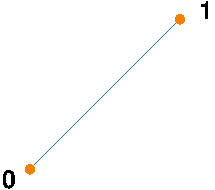
\includegraphics{runpylith/figs/bar2} 
\par\end{centering}

\caption{Linear bar cell available for 1D problems.}


\label{fig:1D-linear-elements} 
\end{figure}

\par\end{center}

\noindent \begin{center}
\begin{figure}[H]
\noindent \begin{centering}
\includegraphics{runpylith/figs/tri3}\hspace*{0.5in}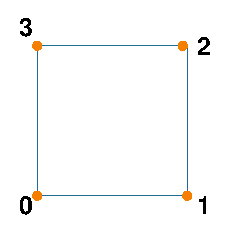
\includegraphics{runpylith/figs/quad4}
\par\end{centering}

\caption{Linear cells available for 2D problems are the triangle (left) and
the quadrilateral (right).}


\label{fig:2D-linear-elements} 
\end{figure}

\par\end{center}

\noindent \begin{center}
\begin{figure}[H]
\noindent \begin{centering}
\includegraphics{runpylith/figs/tet4}\hspace*{0.5in}\includegraphics{runpylith/figs/hex8}
\par\end{centering}

\caption{Linear cells available for 3D problems are the tetrahedron (left)
and the hexahedron (right).\label{fig:3D-linear-elements}}
\end{figure}

\par\end{center}


\subsubsection{Mesh Importer}

The default mesher component is MeshImporter, which provides the capabilities
of reading the mesh from files. The MeshImporter has several properties
and facilities:
\begin{description}
\item [{reorder\_mesh}] Reorder the vertices and cells using the reverse
Cuthill-McKee algorithm (default is False).
\item [{reader}] Reader for a given type of mesh (default is MeshIOAscii).
\item [{distributor}] Handles distribution of the mesh among processors.
\item [{refiner}] Perform global uniform mesh refinement after distribution
among processors (default is False).
\end{description}
Reordering the mesh so that vertices and cells connected topologically
also reside close together in memory improves overall performance
and can improve solver performance as well.
\begin{quote}
\textbf{\textcolor{red}{Warning}}\textcolor{red}{:} The coordinate
system associated with the mesh must be a Cartesian coordinate system.
This includes generic Cartesian coordinate systems as well as geographic
projections.
\end{quote}

\subsubsection{MeshIOAscii}

The MeshIOAscii object is intended for reading small, simple ASCII
files containing a mesh constructed by hand. We use this file format
extensively in the examples. Appendix \ref{sec:MeshIOAscii} describes
the format of the files. The properties and facilities of the MeshIOAscii
object include:
\begin{description}
\item [{filename}] Name of the mesh file.
\item [{coordsys}] Coordinate system associated with the mesh.
\end{description}

\subsubsection{\label{sec:MeshIOCubit}MeshIOCubit}

The MeshIOCubit object reads the NetCDF Exodus II files output from
CUBIT. Beginning with CUBIT 11.0, the names of the nodesets are included
in the Exodus II files and PyLith can use these nodeset names or revert
to using the nodeset ids. The properties and facilities associated
with the MeshIOCubit object are:
\begin{description}
\item [{filename}] Name of the Exodus II file.
\item [{use\_nodeset\_names}] Identify nodesets by name rather than id
(default is True).
\item [{coordsys}] Coordinate system associated with the mesh.
\end{description}

\subsubsection{\label{sec:MeshIOLagrit}MeshIOLagrit}

The MeshIOLagrit object is used to read ASCII and binary GMV and PSET
files output from LaGriT. PyLith will automatically detect whether
the files are ASCII or binary. We attempt to provide support for experimental
64-bit versions of LaGriT via flags indicating whether the FORTRAN
code is using 32-bit or 64-bit integers. The MeshIOLagrit properties
and facilities are:
\begin{description}
\item [{filename\_gmv}] Name of GMV file.
\item [{filename\_pset}] Name of the PSET file.
\item [{flip\_endian}] Flip the endian of values when reading binary files
(default is False).
\item [{io\_int32}] Flag indicating that PSET files use 32-bit integers
(default is True).
\item [{record\_header\_32bt}] Flag indicating FORTRAN record header is
32-bit (default is True)
\item [{coordsys}] Coordinate system associated with mesh.\end{description}
\begin{quote}
\textbf{\textcolor{red}{Warning}}: The PyLith developers have not
used LaGriT since around 2008 and the most recent release appears
to have been in 2010.
\end{quote}

\subsubsection{Distributor}

The distributor users a partitioner to compute which cells should
be placed on each processor, computes the overlap among the processors,
and then distributes the mesh among the processors. The type of partitioner
is set via PETSc settings. The properties and facilities of the Distributor
include:
\begin{description}
\item [{writer\_partition}] Flag indicating that the partition information
should be written to a file (default is False).
\item [{data\_writer}] Writer for partition information (default is DataWriterVTKMesh
for VTK output).
\end{description}
An example of setting the partitioner in a pylithapp.cfg file is:
\begin{lyxcode}
{[}pylithapp.petsc{]}

petscpartitioner~=~chaco~;~Options~are~'chaco'~(default)~and~'parmetis'.
\end{lyxcode}
METIS/ParMETIS are not included in the PyLith binaries due to licensing
issues. 


\subsubsection{Refiner}

The refiner is used to decrease node spacing by a power of two by
recursively subdividing each cell by a factor of two. In a 2D triangular
mesh a node is inserted at the midpoint of each edge, splitting each
cell into four cells (see Figure \ref{fig:uniform:refinement:2x}).
In a 2D quadrilateral mesh a node is inserted at the midpoint of each
edge and at the centroid of the cell, splitting each cell into four
cells. In a 3D tetrahedral mesh a node is inserted at the midpoint
of each edge, splitting each cell into eight cells. In a 3D hexahedral
mesh a node is inserted at the midpoint of each edge, the centroid
of each face, and at the centroid of the cell, splitting each cell
into eight cells.

\noindent \begin{center}
\begin{figure}[H]
\noindent \begin{centering}
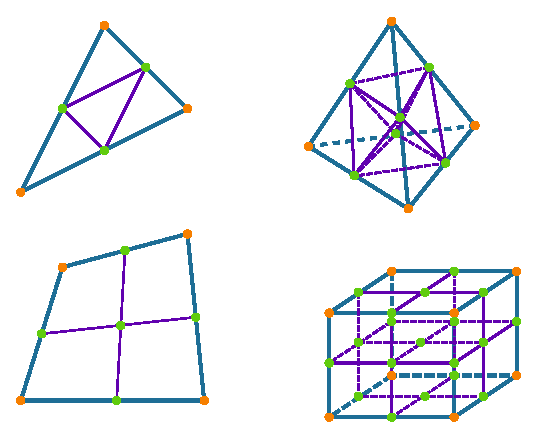
\includegraphics[scale=1.25]{runpylith/figs/refinement2x}
\par\end{centering}

\caption{Global uniform mesh refinement of 2D and 3D linear cells. The blue
lines and orange circles identify the edges and vertices in the original
cells. The purple lines and green circles identify the new edges and
vertices added to the original cells to refine the mesh by a factor
of two.\label{fig:uniform:refinement:2x}}
\end{figure}

\par\end{center}

Refinement occurs after distribution of the mesh among processors.
This allows one to run much larger simulations by (1) permitting the
mesh generator to construct a mesh with a node spacing largeer than
that needed in the simulation and (2) operations performed in serial
during the simulation setup phase, such as, adjusting the topology
to insert cohesive cells and distribution of the mesh among processors
uses this much smaller coarse mesh. For 2D problems the global mesh
refinement increases the maximum problem size by a factor of $4^{n}$,
and for 3D problems it increases the maximum problem size by a factor
of $8^{n}$, where $n$ is the number of recursive refinement levels.
For a tetrahedral mesh, the element quality decreases with refinement
so $n$ should be limited to 1-2.


\subsection{Problem Specification (\texttt{problem})}

The problem component specifies the basic parameters of the simulation,
including the physical properties, the boundary conditions, and interface
conditions (faults). The current release of PyLith contains two types
of problem, \texttt{TimeDependent} for use in static, quasi-static,
and dynamic simulations and \texttt{GreensFns} for computing static
Green's functions. The general facilities include:
\begin{description}
\item [{normalizer}] Scales used to nondimensionalize the problem (default
is NondimElasticQuasistatic).
\item [{materials}] Array of materials comprising the domain (default is
\texttt{{[}material{]}}).
\item [{bc}] Array of boundary conditions (default is none).
\item [{interfaces}] Array of interface conditions, i.e., faults (default
is none).
\item [{gravity\_field}] Gravity field used to construct body forces (default
is none).
\end{description}
The properties for each material group are:
\begin{description}
\item [{dimension}] Spatial dimension of the problem (default is 3)
\end{description}
An example of setting these parameters in a \texttt{.cfg} file for
a problem is:
\begin{lyxcode}
{[}pylithapp.timedependent{]}

dimension~=~3

normalizer~=~spatialdata.units.NondimElasticQuasistatic

materials~=~{[}elastic,viscoelastic{]}

bc~=~{[}boundary\_east,boundary\_bottom,boundary\_west{]}

interfaces~=~{[}SanAndreas,SanJacinto{]}

gravity\_field~=~spatialdata.spatialdb.GravityField
\end{lyxcode}

\subsubsection{Nondimensionalization}

PyLith nondimensionalizes all parameters provided by the user so that
the simulation solves the equations using nondimensional quantities.
This permits application of PyLith to problems across a vast range
of spatial and temporal scales. The scales used to nondimensionalize
the problem are length, pressure, density, and time. PyLith provides
two normalizer objects to make it easy to provide reasonable scales
for the nondimensionalization. The \texttt{NondimElasticQuasistatic}
normalizer (which is the default) has the following properties:
\begin{description}
\item [{length\_scale}] Length to nondimensionalize length (default is
1.0 km).
\item [{shear\_modulus}] Shear modulus to nondimensionalize pressure (default
is 3.0e+10 Pa).
\item [{relaxation\_time}] Relaxation time to nondimensionalize time (default
is 1.0 year).
\end{description}
An example of setting these parameters in a \texttt{.cfg} file for
a problem is:
\begin{lyxcode}
{[}pylithapp.timedependent.normalizer{]}

length\_scale~=~1.0{*}km

shear\_modules~=~3.0e+10{*}Pa

relaxation\_time~=~1.0{*}yr
\end{lyxcode}
The \texttt{NondimElasticDynamic} normalizer has the following properties:
\begin{description}
\item [{shear\_wave\_speed}] Shear wave speed used to nondimensionalize
length and pressure (default is 3.0 km/s).
\item [{mass\_density}] Mass density to nondimensionalize density and pressure
(default is 3.0e+3 kg/m$^{3}$).
\item [{wave\_period}] Period of seismic waves used to nondimensionalize
time (default is 1.0 s).
\end{description}
An example of setting these parameters in a \texttt{.cfg} file for
a problem is:
\begin{lyxcode}
{[}pylithapp.timedependent.normalizer{]}

shear\_wave\_speed~=~3.0{*}km/s

mass\_density~=~3.0e+3{*}kg/m{*}{*}3

wave\_period~=~1.0{*}s
\end{lyxcode}
The default nondimensionalization is reasonable for many problems;
however, it may be necessary to change the default values in some
cases. When doing this, keep in mind that the nondimensionalization
generally applies to the minimum values encountered for a problem.
For example, in a quasistatic problem, the \texttt{length\_scale}
should be on the order of the minimum cell size. Similarly, the \texttt{relaxation\_time}
should be on the order of the minimum relaxation time.


\subsection{Finite-Element Integration Settings}

PyLith uses numerical quadrature to evaluate the finite-element integrals
for the residual and system Jacobian (see Chapter \ref{cha:Governing-Equations}).
PyLith employs FIAT (finite element automatic tabulator) to compute
the basis functions and their derivatives at the quadrature points
for various quadrature schemes and cell shapes. The parameters for
Lagrange cells (lines, quadrilaterals, hexahedra) are specified using
the FIATLagrange object, whereas the parameters for Simplex cells
(lines, triangles, tetrahedra) are specified using the FIATSimplex
object. Both objects use the same set of parameters and PyLith will
setup the basis functions and quadrature scheme appropriately for
the two families of cells. The quadrature scheme and basis functions
must be set for each material and boundary condition involving finite-element
integrations (Dirichlet boundary conditions are constraints and do
not involve integrations). Furthermore, the integration schemes can
be set independently. The current version of PyLith supports basis
functions with linear variations in the field (P1); support for higher
order cells will be added in the future. The properties for the FIATLagrange
and FIATSimplex objects are
\begin{description}
\item [{dimension}] Dimension of the cell (0,1,2,3; default is 3).
\item [{degree}] Degree of the finite-element cell (default is 1).
\item [{order}] Order of quadrature rule (default is degree+1); hardwired
to be equal to degree for faults.
\item [{collocate\_quad}] Collocate quadrature points with vertices (default
is False); hardwired to True for faults.
\end{description}
See Section \ref{sec:material:parameters} for an example of setting
these properties for a material.


\subsection{\label{sec:petsc:options}PETSc Settings (\texttt{petsc})}

In quasti-static problems with implicit time-stepping, PyLith relies
on PETSc for the linear algebra computations, including linear Krylov
subspace solvers and nonlinear solvers. For dynamic problems, lumping
the mass matrix and using explicit time-stepping is much more efficient;
this permits solving the linear system with a trivial solver so we
do not use a PETSc solver in this case (see Section \ref{sec:solvers}).

PETSc options can be set in \texttt{.cfg} files in sections beginning
with \texttt{{[}pylithapp.petsc{]}}. The options of primary interest
in the case of PyLith are shown in Table~\ref{tab:petsc:options:defaults}.
PETSc options are used to control the selection and settings for the
solvers underlying the SolverLinear and SolverNonlinear objects discussed
in Section \ref{sec:solvers}. A very wide range of elasticity problems
in quasi-static simulations can be solved with reasonable runtimes
by replacing the default Jacobi preconditioner with the Additive Schwarz
Method (ASM) using Incomplete LU (ILU) factorization by default (see
Table~\ref{tab:petsc:options:recommended}). A more advanced set
of solver settings that may provide better performance in many elasticity
problems are given in Table \ref{tab:petsc:options:advanced}. These
are available in \texttt{\$PYLITH\_DIR/share/settings/solver\_fault\_fieldsplit.cfg.}
These settings are limited to problems where we store the stiffness
matrix as a nonsymmetric sparse matrix and require additional settings
for the formulation,
\begin{lyxcode}
{[}pylithapp.timedependent.formulation{]}

split\_fields~=~True

use\_custom\_constraint\_pc~=~True~;~Use~only~if~problem~contains~a~fault

matrix\_type~=~aij\end{lyxcode}
\begin{quote}
\textbf{\textcolor{red}{Warning:}}\textbf{ }These settings are only
available if you build PETSc with the ML package. These features are
included in the PyLith binary packages.

\textbf{\textcolor{red}{Warning:}}\textbf{ }The split fields and algebraic
multigrid preconditioning currently fails in problems with a nonzero
null space. This most often occurs when a problem contains multiple
faults that extend through the entire domain and create subdomains
without any Dirichlet boundary conditions. The current workaround
is to use the Additive Schwarz preconditioner without split fields.
See Section \ref{sec:Troubleshooting} for the error message encountered
in this situation. 
\end{quote}
These more advanced settings allow the displacement fields and Lagrange
multipliers for fault tractions to be preconditioned separately. This
usually results in a much stronger preconditioner. In simulations
with fault slip, the degrees of freedom associated with the Lagrange
multipliers should be preconditioned with a custom preconditioner
that uses a diagonal approximation of the Schur complement.

\noindent \begin{center}
\begin{table}[H]
\centering{}\caption{\label{tab:petsc:options:defaults}Useful command-line arguments for
setting PETSc options.}
\begin{tabular}{|>{\raggedright}p{1.2in}|>{\centering}m{0.6in}|>{\raggedright}p{3.8in}|}
\hline 
\textbf{Property} & \textbf{Default Value} & \textbf{Description}\tabularnewline
\hline 
\hline 
\texttt{log\_view} & \textit{false} & Print logging objects and events.\tabularnewline
\hline 
\texttt{ksp\_monitor} & \textit{false} & Dump preconditioned residual norm to stdout.\tabularnewline
\hline 
\texttt{ksp\_view} & \textit{false} & Print linear solver parameters. \tabularnewline
\hline 
\texttt{ksp\_rtol} & \textit{1.0e-05} & Convergence tolerance for relative decrease in residual norm.\tabularnewline
\hline 
\texttt{snes\_monitor} & \textit{false} & Dump residual norm to stdout for each nonlinear solve iteration.\tabularnewline
\hline 
\texttt{snes\_view} & \textit{false} & Print nonlinear solver parameters.\tabularnewline
\hline 
\texttt{snes\_rtol} & \textit{1.0e-5} & Convergence tolerance for relative decrease in residual norm.\tabularnewline
\hline 
\texttt{pc\_type} & \textit{jacobi} & Set preconditioner type. See \href{http://www.mcs.anl.gov/petsc/petsc-as/documentation/linearsolvertable.html}{PETSc documentation}
for a list of all preconditioner types. \tabularnewline
\hline 
\texttt{ksp\_type} & \textit{gmres} & Set linear solver type. See \href{http://www.mcs.anl.gov/petsc/petsc-as/documentation/linearsolvertable.html}{PETSc documentation}
for a list of all solver types.\tabularnewline
\hline 
\end{tabular}
\end{table}
\begin{table}[H]
\centering{}\caption{\label{tab:petsc:options:recommended}PETSc options that provide moderate
performance in a wide range of quasi-static elasticity problems.}
\begin{tabular}{|>{\raggedright}p{2in}|>{\centering}m{0.75in}|>{\raggedright}p{3in}|}
\hline 
\textbf{Property} & \textbf{Value} & \textbf{Description}\tabularnewline
\hline 
\hline 
\texttt{pc\_type} & \textit{asm} & Additive Schwarz method.\tabularnewline
\hline 
\texttt{ksp\_type} & \textit{gmres} & GMRES method from Saad and Schultz.\tabularnewline
\hline 
\texttt{sub\_pc\_factor\_shift\_type} & \emph{nonzero} & Turn on nonzero shifting for factorization.\tabularnewline
\hline 
\texttt{ksp\_max\_it} & \emph{100} & Maximum number of iterations permitted in linear solve. Depends on
problem size.\tabularnewline
\hline 
\texttt{ksp\_gmres\_restart} & \textit{50} & Number of iterations after which Gram-Schmidt orthogonalization is
restarted.\tabularnewline
\hline 
\texttt{ksp\_rtol} & \textit{1.0e-08} & Linear solve convergence tolerance for relative decrease in residual
norm.\tabularnewline
\hline 
\texttt{ksp\_atol} & \textit{\emph{1.0e-12}} & Linear solve convergence tolerance for absolute value of residual
norm.\tabularnewline
\hline 
\texttt{ksp\_converged\_reason} & \textit{true} & Indicate why iterating stopped in linear solve.\tabularnewline
\hline 
\texttt{snes\_max\_it} & \textit{100} & Maximum number of iterations permitted in nonlinear solve. Depends
on how nonlinear the problem is.\tabularnewline
\hline 
\texttt{snes\_rtol} & \textit{1.0e-08} & Nonlinear solve convergence tolerance for relative decrease in residual
norm.\tabularnewline
\hline 
\texttt{snes\_atol} & \textit{1.0e-12} & Nonlinear solve convergence tolerance for absolute value of residual
norm.\tabularnewline
\hline 
\texttt{snes\_converged\_reason} & \textit{true} & Indicate why iterating stopped in nonlinear solve.\tabularnewline
\hline 
\end{tabular}
\end{table}

\par\end{center}

\noindent \begin{center}
\begin{table}[H]
\centering{}\caption{\label{tab:petsc:options:advanced}PETSc options used with split fields
algebraic multigrid preconditioning that often provide improved performance
in quasi-static elasticity problems with faults.}
\begin{tabular}{|>{\raggedright}p{2.75in}|>{\centering}m{0.75in}|>{\raggedright}p{2.5in}|}
\hline 
\textbf{Property} & \textbf{Value} & \textbf{Description}\tabularnewline
\hline 
\hline 
\texttt{\footnotesize{}fs\_pc\_type} & \textit{field\_split} & Precondition fields separately.\tabularnewline
\hline 
\texttt{\footnotesize{}fs\_pc\_use\_amat} & \textit{true} & Use diagonal blocks from the true operator, rather than the preconditioner.\tabularnewline
\hline 
\texttt{\footnotesize{}fs\_pc\_fieldsplit\_type} & \textit{multiplicative} & Apply each field preconditioning in sequence, which is stronger than
all-at-once (additive).\tabularnewline
\hline 
\texttt{\footnotesize{}fs\_fieldsplit\_displacement\_pc\_type} & \textit{ml} & Multilevel algebraic multigrid preconditioning using Trilinos/ML via
PETSc.\tabularnewline
\hline 
\texttt{\footnotesize{}fs\_fieldsplit\_lagrange\_multiplier\_pc\_type} & \textit{jacobi} & Jacobi preconditioning for Lagrange multiplier block\tabularnewline
\hline 
\texttt{\footnotesize{}fs\_fieldsplit\_displacement\_ksp\_type} & \textit{preonly} & Apply only the preconditioner.\tabularnewline
\hline 
\texttt{\footnotesize{}fs\_fieldsplit\_lagrange\_multiplier\_ksp\_type} & \textit{preonly} & Apply only the preconditioner.\tabularnewline
\hline 
\end{tabular}
\end{table}

\par\end{center}


\subsubsection{Model Verification with PETSc Direct Solvers}

It is often useful to apply a direct solver so that solver convergence
is decoupled from model verification for the purposes of testing.
Unfortunately, the traditional LU factorization solvers cannot be
directly applied in PyLith due to the saddle-point formulation used
to accomodate the fault slip constraints. However, we can combine
an LU factorization of the displacement sub-block with a full Schur
complement factorization using the PETSc FieldSplit preconditioner.
If the solver for the Schur complement S is given a very low tolerance,
this is effectively a direct solver. The options given below will
construct this solver in PyLith. These settings are available in\texttt{}~\\
\texttt{\$PYLITH\_DIR/share/settings/solver\_fault\_exact.cfg}.
\begin{lyxcode}
{[}pylithapp.timedependent.formulation{]}

split\_fields~=~True

matrix\_type~=~aij



{[}pylithapp.petsc{]}

fs\_pc\_type~=~fieldsplit

fs\_pc\_use\_amat~=~True

fs\_pc\_fieldsplit\_type~=~schur

fs\_pc\_fieldsplit\_schur\_factorization\_type~=~full

fs\_fieldsplit\_displacement\_ksp\_type~=~preonly

fs\_fieldsplit\_displacement\_pc\_type~=~lu

fs\_fieldsplit\_lagrange\_multiplier\_pc\_type~=~jacobi

fs\_fieldsplit\_lagrange\_multiplier\_ksp\_type~=~gmres

fs\_fieldsplit\_lagrange\_multiplier\_ksp\_rtol~=~1.0e-11
\end{lyxcode}

\section{Time-Dependent Problem}

This type of problem applies to transient static, quasi-static, and
dynamic simulations. The time-dependent problem adds the \texttt{formulation}
facility to the general-problem. The formulation specifies the time-stepping
formulation to integrate the elasticity equation. PyLith provides
several alternative formulations, each specific to a different type
of problem.
\begin{description}
\item [{Implicit}] Implicit time stepping for static and quasi-static problems
with infinitesimal strains. The implicit formulation neglects inertial
terms (see Section \ref{eq:elasticity:integral:quasistatic}). 
\item [{ImplicitLgDeform}] Implicit time stepping for static and quasi-static
problems including the effects of rigid body motion and small strains.
This formulation requires the use of the nonlinear solver, which is
selected automatically.
\item [{Explicit}] Explicit time stepping for dynamic problems with infinitesimal
strains and lumped system Jacobian. The cell matrices are lumped before
assembly, permitting use of a vector for the diagonal system Jacobian
matrix. The built-in lumped solver is selected automatically.
\item [{ExplicitLgDeform}] Explicit time stepping for dynamic problems
including the effects of rigid body motion and small strains. The
cell matrices are lumped before assembly, permitting use of a vector
for the diagonal system Jacobian matrix. The built-in lumped solver
is selected automatically.
\item [{ExplicitTri3}] Optimized elasticity formulation for linear triangular
cells with one point quadrature for dynamic problems with infinitesimal
strains and lumped system Jacobian. The built-in lumped solver is
selected automatically.
\item [{ExplicitTet4}] Optimized elasticity formulation for linear tetrahedral
cells with one point quadrature for dynamic problems with infinitesimal
strains and lumped system Jacobian.The built-in lumped solver is selected
automatically.
\end{description}
In many quasi-static simulations it is convenient to compute a static
problem with elastic deformation prior to computing a transient response.
Up through PyLith version 1.6 this was hardwired into the Implicit
Forumulation as advancing from time step $t=-\Delta t$ to $t=0$,
and it could not be turned off. PyLith now includes a property, \texttt{elastic\_prestep}
in the TimeDependent component to turn on/off this behavior (the default
is to retain the previous behavior of computing the elastic deformation). 
\begin{quote}
\textbf{\textcolor{red}{Warning:}}\textbf{ }Turning off the elastic
prestep calculation means the model only deforms when an \texttt{\textit{increment}}
in loading or deformation is applied, because the time-stepping formulation
is implemented using the increment in displacement.
\end{quote}
The TimeDependent properties and facilities include
\begin{description}
\item [{elastic\_preset}] If true, perform a static calculation with elastic
behavior before time stepping (default is True).
\item [{formulation}] Formulation for solving the partial differential
equation.
\item [{progress\_monitor}] Simple progress monitor via text file.
\end{description}
An example of setting the properties and components in a .cfg file
is
\begin{lyxcode}
{[}pylithapp.timedependent{]}

formulation~=~pylith.problems.Implicit~;~default

progres\_monitor~=~pylith.problems.ProgressMonitorTime~;~default

elastic\_preset~=~True~;~default
\end{lyxcode}
The formulation value can be set to the other formulations in a similar
fashion. 


\subsection{Time-Stepping Formulation}

The explicit and implicit time stepping formulations use a common
set of facilities and properties. The facilities include
\begin{description}
\item [{time\_step}] Time step size specification (default is uniform time
step).
\item [{solver}] Type of solver to use (default is SolverLinear).
\item [{output}] Array of output managers for output of the solution (default
is {[}output{]}).
\item [{jacobian\_viewer}] Viewer to dump the system Jacobian (sparse matrix)
to a file for analysis (default is PETSc binary).
\end{description}
The formulation properties include
\begin{description}
\item [{matrix\_type}] Type of PETSc matrix for the system Jacobian (sparse
matrix, default is symmetric, block matrix with a block size of 1).
\item [{view\_jacobian}] Flag to indicate if system Jacobian (sparse matrix)
should be written to a file (default is false).
\item [{split\_fields}] Split solution field into a displacement portion
(fields 0..ndim-1) and a Lagrange multiplier portion (field ndim)
to permit application of sophisticated PETSc preconditioners (default
is false).
\end{description}
An example of setting these parameters in a \texttt{.cfg} file is
\begin{lyxcode}
{\footnotesize{}{[}pylithapp.timedependent.formulation{]}}{\footnotesize \par}

{\footnotesize{}time\_step~=~pylith.problems.TimeStepUniform}{\footnotesize \par}

{\footnotesize{}solver~=~pylith.problems.SolverLinear~;~Nonlinear~solver~is~pylith.problems.SolverNonlinear}{\footnotesize \par}

{\footnotesize{}output~=~{[}domain,ground\_surface{]}}{\footnotesize \par}

{\footnotesize{}matrix\_type~=~sbaij~;~To~use~a~non-symmetric~sparse~matrix,~set~it~to~aij}{\footnotesize \par}

{\footnotesize{}view\_jacobian~=~false}{\footnotesize \par}
\end{lyxcode}

\subsection{Numerical Damping in Explicit Time Stepping}

In explicit time-stepping formulations for elasticity, boundary conditions
and fault slip can excite short waveform elastic waves that are not
accurately resolved by the discretization. We use numerical damping
via an artificial viscosity\cite{Knopoff:Ni:2001,Day:Ely:2002} to
reduce these high frequency oscillations. In computing the strains
for the elasticity term in equation \ref{eq:elasticity:integral:dynamic:t},
we use an adjusted displacement rather than the actual displacement,
where 
\begin{equation}
\vec{u}^{adj}(t)=\vec{u}(t)+\eta^{*}\Delta t\vec{\dot{u}}(t),
\end{equation}
$\vec{u}^{adj}(t)$ is the adjusted displacement at time t, $\vec{u}(t)$is
the original displacement at time (t), $\eta^{*}$is the normalized
artificial viscosity, $\Delta t$ is the time step, and $\vec{\dot{u}}(t)$
is the velocity at time $t$. The default value for the normalized
artificial viscosity is 0.1. We have found values in the range 0.1-0.4
sufficiently suppress numerical noise while not excessively reducing
the peak velocity. An example of setting the normalized artificial
viscosity in a \texttt{.cfg} file is
\begin{lyxcode}
{[}pylithapp.timedependent.formulation{]}

norm\_viscosity~=~0.2
\end{lyxcode}

\subsection{\label{sec:solvers}Solvers}

PyLith supports three types of solvers. The linear solver, SolverLinear,
corresponds to the PETSc KSP solver and is used in linear problems
with linear elastic and viscoelastic bulk constitutive models and
kinematic fault ruptures. The nonlinear solver, SolverNonlinear, corresponds
to the PETSc SNES solver and is used in nonlinear problems with nonlinear
viscoelastic or elastoplastic bulk constitutive models, dynamic fault
ruptures, or problems involving finite strain (small strain formulation).
The lumped solver (SolverLumped) is a specialized solver used with
the lumped system Jacobian matrix. The options for the PETSc KSP and
SNES solvers are set via the top-level PETSc options (see Section
\ref{sec:petsc:options} and the PETSc documentation \url{www.mcs.anl.gov/petsc/petsc-as/documentation/index.html}).


\subsection{\label{sub:Time-Stepping}Time Stepping}

PyLith provides three choices for controlling the time step in time-dependent
simulations. These include (1) a uniform, user-specified time step
(which is the default), (2) user-specified time steps (potentially
nonuniform), and (3) automatically calculated (potentially nonuniform)
time steps. The procedure for automatically selecting time steps requires
that the material models provide a reasonable estimate of the time
step for stable time integration. In general, quasi-static simulations
with viscoelastic materials should use automatically calculated time
steps and dynamic simulations should use a uniform, user-specified
time step. Note that all three of the time stepping schemes make use
of the computed stable time step (see \ref{sub:Stable-time-step}).
When using user-specified time steps, the value is checked against
the computed stable time step. The automatically calculated time step
comes from the computed stable time step.
\begin{quote}
\textbf{\textcolor{red}{Warning:}} Varying the time step within a
simulation requires recomputing the Jacobian of the system whenever
the time step changes, which can greatly increase the runtime if the
time-step size changes frequently.
\end{quote}

\subsubsection{Uniform, User-Specified Time Step}

With a uniform, user-specified time step, the user selects the time
step that is used over the entire duration of the simulation. If this
value exceeds the computed stable time step at any time, PyLith will
terminate with an error. The properties for the uniform, user-specified
time step are:
\begin{description}
\item [{total\_time}] Time duration for simulation (default is 0.0 s).
\item [{start\_time}] Start time for simulation (default is 0.0 s)
\item [{dt}] Time step for simulation.
\end{description}
An example of setting a uniform, user-specified time step in a \texttt{.cfg}
file is:
\begin{lyxcode}
{[}pylithapp.problem.formulation{]}

time\_step~=~pylith.problems.TimeStepUniform~;~Default~value



{[}pylithapp.problem.formulation.time\_step{]}

total\_time~=~1000.0{*}year

dt~=~0.5{*}year
\end{lyxcode}

\subsubsection{Nonuniform, User-Specified Time Step}

The nonuniform, user-specified, time-step implementation allows the
user to specify the time steps in an ASCII file (see Section \ref{sec:FileFormat:TimeStepUser}
for the format specification of the time-step file). If the total
duration exceeds the time associated with the time steps, then a flag
determines whether to cycle through the time steps or to use the last
specified time step for the time remaining. Similar to the uniform
time step, if the user-specified time step size exceeds the computed
stable time step at any time, PyLith will terminate with an error.
The properties for the nonuniform, user-specified time step are:
\begin{description}
\item [{total\_time}] Time duration for simulation.
\item [{filename}] Name of file with time-step sizes.
\item [{loop\_steps}] If true, cycle through time steps, otherwise keep
using last time-step size for any time remaining.
\end{description}
An example of setting the properties for nonuniform, user-specified
time steps in a \texttt{.cfg} file is:
\begin{lyxcode}
{[}pylithapp.problem.formulation{]}

time\_step~=~pylith.problems.TimeStepUser~;~Change~the~time~step~algorithm



{[}pylithapp.problem.formulation.time\_step{]}

total\_time~=~1000.0{*}year

filename~=~timesteps.txt

loop\_steps~=~false~;~Default~value
\end{lyxcode}

\subsubsection{Nonuniform, Automatic Time Step}

This time-step implementation automatically calculates a time step
size based on the constitutive model and rate of deformation. As a
result, this choice for choosing the time step relies on accurate
calculation of a stable time step within each finite-element cell
by the constitutive models. To provide some control over the time-step
selection, the user can control the frequency with which a new time
step is calculated, the time step to use relative to the value determined
by the constitutive models, and a maximum value for the time step.
Note that the stability factor allows the computed time step size
to exceed the computed stable time step. A stability factor of 1.0
would provide a time step size equal to the stable time step, while
a value of 2.0 (default value) would provide a time step size equal
to 1/2 the stable time step. Caution should be used when adjusting
the stability factor to values less than 1.0, as the large time step
size may result in inaccurate solutions. The properties for controlling
the automatic time-step selection are:
\begin{description}
\item [{total\_time}] Time duration for simulation.
\item [{max\_dt}] Maximum time step permitted.
\item [{adapt\_skip}] Number of time steps to skip between calculating
new stable time step.
\item [{stability\_factor}] Safety factor for stable time step (default
is 2.0).
\end{description}
An example of setting the properties for the automatic time step in
a \texttt{.cfg} file is:
\begin{lyxcode}
{[}pylithapp.problem.formulation{]}

time\_step~=~pylith.problems.TimeStepAdapt~;~Change~the~time~step~algorithm



{[}pylithapp.problem.formulation.time\_step{]}

total\_time~=~1000.0{*}year

max\_dt~=~10.0{*}year

adapt\_skip~=~10~;~Default~value

stability\_factor~=~2.0~;~Default~value
\end{lyxcode}

\section{Green's Functions Problem}

This type of problem applies to computing static Green's functions
for elastic deformation. The \texttt{GreensFns} problem specializes
the time-dependent facility to the case of static simulations with
slip impulses on a fault. The default formulation is the Implicit
formulation and should not be changed as the other formulations are
not applicable to static Green's functions. In the output files, the
deformation at each ``time step'' is the deformation for a different
slip impulse. The properties provide the ability to select which fault
to use for slip impulses. The only fault component available for use
with the \texttt{GreensFns} problem is the \texttt{FaultCohesiveImpulses}
component discussed in Section \ref{sec:fault:cohesive:impulses}.
The \texttt{GreensFns} properties amd facilities include:
\begin{description}
\item [{fault\_id}] Id of fault on which to impose slip impulses.
\item [{formulation}] Formulation for solving the partial differential
equation.
\item [{progress\_monitor}] Simple progress monitor via text file.
\end{description}
An example of setting the properties for the GreensFns problem in
a \texttt{.cfg} file is:
\begin{lyxcode}
{[}pylithapp{]}

problem~=~pylith.problems.GreensFns~;~Change~problem~type~from~the~default



{[}pylithapp.greensfns{]}

fault\_id~=~100~;~Default~value

formulation~=~pylith.problems.Implicit~;~default

progres\_monitor~=~pylith.problems.ProgressMonitorTime~;~default

\end{lyxcode}
\begin{quote}
\textbf{\textcolor{red}{Warning:}} The \texttt{GreensFns} problem
generates slip impulses on a fault. The current version of PyLith
requires that impulses can only be applied to a single fault and the
fault facility must be set to \texttt{FaultCohesiveImpulses}.
\end{quote}

\section{Progress Monitors}
\begin{quotation}
\texttt{\textcolor{red}{New in v2.1.0.}}
\end{quotation}
The progress monitors make it easy to monitor the general progress
of long simulations, especially on clusters where stdout is not always
easily accessible. The progress monitors update a simulation's current
progress by writing information to a text file. The information includes
time stamps, percent completed, and an estimate of when the simulation
will finish. 


\subsection{ProgressMonitorTime}

This is the default progress monitor for time-stepping problems. The
monitor calculates the percent completed based on the time at the
current time step and the total simulated time of the simulation,
not the total number of time steps (which may be unknown in simulations
with adaptive time stepping). The \texttt{ProgressMonitorTime} properties
include:
\begin{description}
\item [{update\_percent}] Frequency (in percent) of progress updates.
\item [{filename}] Name of output file.
\item [{t\_units}] Units for simulation time in output.
\end{description}
An example of setting the properties in a .\texttt{cfg} file is:
\begin{lyxcode}
{[}pylithapp.problem.progressmonitor{]}

update\_percent~=~5.0~;~default

filename~=~progress.txt~;~default

t\_units~=~year~;~default
\end{lyxcode}

\subsection{ProgressMonitorStep}

This is the default progress monitor for problems with a specified
number of steps, such as Green's function problems. The monitor calculates
the percent completed based on the number of steps (e.g., Green's
function impulses completed). The ProgressMonitorStep propertiles
include:
\begin{description}
\item [{update\_percent}] Frequency (in percent) of progress updates.
\item [{filename}] Name of output file.
\end{description}
An example of setting the properties in a .\texttt{cfg} file is:
\begin{lyxcode}
{[}pylithapp.problem.progressmonitor{]}

update\_percent~=~5.0~;~default

filename~=~progress.txt~;~default
\end{lyxcode}

\section{\label{sec:spatial:databases}Databases for Boundaries, Interfaces,
and Material Properties}

Once the problem has been defined with PyLith parameters, and the
mesh information has been provided, the final step is to specify the
boundary conditions and material properties to be used. The mesh information
provides labels defining sets of vertices to which boundary conditions
or fault conditions will be applied, as well as cell labels that will
be used to define the material type of each cell. For boundary conditions,
the \texttt{.cfg} file is used to associate boundary condition types
and spatial databases with each vertex group (see Chapter \ref{cha:boundary:interface:conditions}).
For materials, the \texttt{.cfg} file is used to associate material
types and spatial databases with cells identified by the material
identifier (see Figure \ref{fig:Material-models}).

The spatial databases define how the boundary conditions or material
property values vary spatially, and they can be arbitrarily complex.
The simplest example for a material database would be a mesh where
all the cells of a given type have uniform properties (``point''
or 0D variation). A slightly more complex case would be a mesh where
the cells of a given type have properties that vary linearly along
a given direction (``line'' or 1D variation). In more complex models,
the material properties might have different values at each point
in the mesh (``volume'' or 3D variation). This might be the case,
for example, if the material properties are provided by a database
of seismic velocities and densities. For boundary conditions the simplest
case would be where all vertices in a given group have the same boundary
condition parameters (``point'' or 0D variation). A more complex
case might specify a variation in the conditions on a given surface
(``area'' or 2D variation). This sort of condition might be used,
for example, to specify the variation of slip on a fault plane. The
examples discussed in Chapter \ref{cha:Tutorials} also contain more
information regarding the specification and use of the spatial database
files.


\subsection{SimpleDB Spatial Database}

In most cases the default type of spatial database for faults, boundary
conditions, and materials is \texttt{SimpleDB}. Spatial database files
provide specification of a field over some set of points. There is
no topology associated with the points. Although multiple values can
be specified at each point with more than one value included in a
search query, the interpolation of each value will be done independently.
Time dependent variations of a field are not supported in these files.
Spatial database files can specify spatial variations over zero, one,
two, and three dimensions. Zero dimensional variations correspond
to uniform values. One-dimensional spatial variations correspond to
piecewise linear variations, which need not coincide with coordinate
axes. Likewise, two-dimensional spatial variations correspond to variations
on a planar surface (which need not coincide with the coordinate axes)
and three-dimensional spatial variations correspond to variations
over a volume. In one, two, or three dimensions, queries can use a
``nearest value'' search or linear interpolation.

The spatial database files need not provide the data using the same
coordinate system as the mesh coordinate system, provided the two
coordinate systems are compatible. Examples of compatible coordinate
systems include geographic coordinates (longitude/latitude/elevation),
and projected coordinates (e.g., coordinates in a transverse Mercator
projection). Spatial database queries use the Proj.4 Cartographic
Projections library \url{proj.maptools.org} to convert between coordinate
systems, so a large number of geographic projections are available
with support for converting between NAD27 and WGS84 horizontal datums
as well as several other frequently used datums. Because the interpolation
is done in the coordinate system of the spatial database, geographic
coordinates should only be used for very simple datasets, or undesirable
results will occur. This is especially true when the spatial database
coordinate system combines latitude, longitude, and elevation in meters
(longitude and latitude in degrees are often much smaller than elevations
in meters leading to distorted ``distance'' between locations and
interpolation).

SimpleDB uses a simple ASCII file to specify the variation of values
(e.g., displacement field, slip field, physical properties) in space.
The file format is described in Section \ref{sec:Spatialdata:SimpleIOAscii}.
The tutorials in Chapter \ref{cha:Tutorials} use SimpleDB files to
specify the values for the boundary conditions,  physical properties,
and fault slip.

As in the other Pyre objects, spatial database objects contain parameters
that can be set from the command line or using \texttt{.cfg or .pml}
files. The parameters for a spatial database are:
\begin{description}
\item [{label}] Label for the database, which is used in diagnostic messages.
\item [{query\_type}] Type of search query to perform. Values for this
parameter are ``linear'' and ``nearest'' (default).
\item [{iohandler}] Database importer. Only one importer is implemented,
so you do not need to change this setting.
\item [{iohandler.filename}] Filename for the spatial database.
\end{description}
An example of setting these parameters in a \texttt{.cfg} file is:
\begin{lyxcode}
label~=~Material~properties

query\_type~=~linear

iohandler.filename~=~mydb.spatialdb


\end{lyxcode}

\subsection{UniformDB Spatial Database}

The SimpleDB spatial database is quite general, but when the values
are uniform, it is often easier to use the UniformDB spatial database
instead. With the UniformDB, you specify the values directly either
on the command line or in a parameter-setting (\texttt{.cfg}) file.
On the other hand, if the values are used in more than one place,
it is easier to place the values in a SimpleDB file, because they
can then be referred to using the filename of the spatial database
rather than having to repeatedly list all of the values on the command
line or in a parameter-setting (\texttt{.cfg}) file. The Pyre properties
for a UniformDB are:
\begin{description}
\item [{values}] Array of names of values in spatial database
\item [{data}] Array of values in spatial database
\end{description}

\subsubsection{Example}

Specify the physical properties of a linearly elastic, isotropic material
in a \texttt{pylithapp.cfg} file. The data values are dimensioned
with the appropriate units using Python syntax.
\begin{lyxcode}
{\footnotesize{}{[}pylithapp.timedependent.materials.material{]}}{\footnotesize \par}

{\footnotesize{}db\_properties~=~spatialdata.spatialdb.UniformDB~;~Set~the~db~to~a~UniformDB}{\footnotesize \par}

{\footnotesize{}db\_properties.values~=~{[}vp,vs,density{]}~;~Set~the~names~of~the~values~in~the~database}{\footnotesize \par}

{\footnotesize{}db\_properties.data~=~{[}5773.5{*}m/s,~3333.3{*}m/s,~2700.0{*}kg/m{*}{*}3{]}~;~Set~the~values~in~the~database}{\footnotesize \par}
\end{lyxcode}

\subsubsection{ZeroDispDB}

The ZeroDispDB is a a special case of the UniformDB for the Dirichlet
boundary conditions. The values in the database are the ones requested
by the Dirichlet boundary conditions, \texttt{displacement-x}, \texttt{displacement-y},
and \texttt{displacement-z}, and are all set to zero. This makes it
trivial to set displacements to zero on a boundary. The examples discussed
in Chapter \ref{cha:Tutorials} use this database.


\subsection{SimpleGridDB Spatial Database}

The SimpleGridDB object provides a much more efficient query algorithm
than SimpleDB in cases with a orthogonal grid. The points do not need
to be uniformly spaced along each coordinate direction. Thus, in contrast
to the SimpleDB there is an implicit topology. Nevertheless, the points
can be specified in any order, as well as over a lower-dimension than
the spatial dimension. For example, one can specify a 2-D grid in
3-D space provided that the 2-D grid is aligned with one of the coordinate
axes. 

SimpleGridDB uses a simple ASCII file to specify the variation of
values (e.g., displacement field, slip field, physical properties)
in space. The file format is described in Section \ref{sec:Spatialdata:SimpleGrid}. 

As in the other Pyre objects, spatial database objects contain parameters
that can be set from the command line or using \texttt{.cfg or .pml}
files. The parameters for a spatial database are:
\begin{description}
\item [{label}] Label for the database, which is used in diagnostic messages.
\item [{query\_type}] Type of search query to perform. Values for this
parameter are ``linear'' and ``nearest'' (default).
\item [{filename}] Filename for the spatial database.
\end{description}
An example of setting these parameters in a \texttt{.cfg} file is:
\begin{lyxcode}
label~=~Material~properties

query\_type~=~linear

filename~=~mydb\_grid.spatialdb


\end{lyxcode}

\subsection{\label{sub:SCECCVMH-Impl}SCEC CVM-H Spatial Database}

Although the SimpleDB implementation is able to specify arbitrarily
complex spatial variations, there are existing databases for physical
properties, and when they are available, it is desirable to access
these directly. One such database is the SCEC CVM-H database, which
provides seismic velocities and density information for much of southern
California. Spatialdata provides a direct interface to this database.
See Section \ref{sec:Tutorial-Two-tet4-geoproj} for an example of
using the SCEC CVM-H database for physical properties of an elastic
material. The interface is known to work with versions 5.2 and 5.3
of the SCEC CVM-H. Setting a minimum wave speed can be used to replace
water and very soft soils that are incompressible or nearly incompressible
with stiffer, compressible materials. The Pyre properties for the
SCEC CVM-H are:
\begin{description}
\item [{data\_dir}] Directory containing the SCEC CVM-H data files
\item [{min\_vs}] Minimum shear wave speed. Corresponding minimum values
for the dilatational wave speed (Vp) and density are computed. Default
value is 500 m/s.
\item [{squash}] Squash topography/bathymetry to sea level (make the earth's
surface flat)
\item [{squash\_limit}] Elevation above which topography is squashed (geometry
below this elevation remains undistorted)
\end{description}

\subsubsection{Example}

Specify the physical properties of a linearly elastic, isotropic material
using the SCEC CVM-H in a \texttt{pylithapp.cfg} file.
\begin{lyxcode}
{\small{}{[}pylithapp.timedependent.materials.material{]}}{\small \par}

{\small{}db\_properties~=~spatialdata.spatialdb.SCECCVMH~;~Set~the~database~to~the~SCEC~CVM-H}{\small \par}

{\small{}db\_properties.data\_dir~=~/home/johndoe/data/sceccvm-h/vx53~;~Directory~containing}~\\
{\small{}the~database~data~files}{\small \par}

{\small{}db\_properties.min\_vs~=~500{*}m/s}{\small \par}

{\small{}db\_properties.squash~=~True~;~Turn~on~squashing}{\small \par}

{\small{}db\_properties.squash\_limit~=~-1000.0~;~Only~distort~the~geometry~above~z~=~-1~km~in~}~\\
{\small{}flattening~the~earth}{\small \par}
\end{lyxcode}

\subsection{CompositeDB Spatial Database}

For some problems, a boundary condition or material property may have
subsets with different spatial variations. One example would be when
we have separate databases to describe the elastic and inelastic bulk
material properties for a region. In this case, it would be useful
to have two different spatial databases, e.g., a seismic velocity
model with Vp, Vs, and density values, and another database with the
inelastic physical properties. We can use the \texttt{CompositeDB}
spatial database for these cases. An example would be:
\begin{lyxcode}
{[}pylithapp.timedependent.materials.maxwell{]}

label~=~Maxwell~material

id~=~1

db\_properties~=~spatialdata.spatialdb.CompositeDB

db\_properties.db\_A~=~spatialdata.spatialdb.SCECCVMH

db\_properties.db\_B~=~spatialdata.spatialdb.SimpleDB

quadrature.cell~=~pylith.feassemble.FIATSimplex

quadrature.cell.dimension~=~3

~

{[}pylithapp.timedependent.materials.maxwell.db\_properties{]}

values\_A~=~{[}density,vs,vp{]}

db\_A.label~=~Elastic~properties~from~CVM-H

db\_A.data\_dir~=~/Users/willic3/geoframe/tools/vx53/bin

db\_A.squash~=~False

values\_B~=~{[}viscosity{]}

db\_B.label~=~Vertically~varying~Maxwell~material

db\_B.iohandler.filename~=~../spatialdb/mat\_vert\_var\_maxwell.spatialdb
\end{lyxcode}
Here we have specified a \texttt{CompositeDB} where the elastic properties
(\texttt{density}, \texttt{vs}, \texttt{vp}) are given by the SCEC
CVM-H, and \texttt{viscosity} is described by a \texttt{SimpleDB}
(\texttt{mat\_vert\_var\_maxwell.spatialdb}). The user must first
specify \texttt{db\_properties} as a \texttt{CompositeDB}, and must
then give the two components of this database (\texttt{SCECCVMH} and
\texttt{SimpleDB}). The values to query in each of these databases
is also required. This is followed by the usual parameters for each
of the spatial databases. The \texttt{CompositeDB} provides a flexible
mechanism for specifying material properties or boundary conditions
where the variations come from two different sources.


\subsection{Time History Database}

The time history database specifies the temporal variation in the
amplitude of a field associated with a boundary condition. It is used
in conjunction with spatial databases to provide spatial and temporal
variation of parameters for boundary conditions. The same time history
is applied to all of the locations, but the time history may be shifted
with a spatial variation in the onset time and scaled with a spatial
variation in the amplitude. The time history database uses a simple
ASCII file which is simpler than the one used by the SimpleDB spatial
database. The file format is described in Section \ref{sec:Spatialdata:TimeHistoryIO}. 

As in the other Pyre objects, spatial database objects contain parameters
that can be set from the command line or using \texttt{.cfg or .pml}
files. The parameters for a spatial database are:
\begin{description}
\item [{label}] Label for the time history database, which is used in diagnostic
messages.
\item [{filename}] Filename for the time history database.
\end{description}
An example of setting these parameters in a \texttt{.cfg} file is:
\begin{lyxcode}
label~=~Displacement~time~history

filename~=~mytimehistory.timedb
\end{lyxcode}

\section{Labels and Identifiers for Materials, Boundary Conditions, and Faults}

For materials, the ``label'' is a string used only for error messages.
The ``id'' is an integer that corresponds to the material identifier
in LaGriT (itetclr) and CUBIT (block id). The id also tags the cells
in the mesh for associating cells with a specific material model and
quadrature rule. For boundary conditions, the ``label'' is a string
used to associate groups of vertices (psets in LaGriT and nodesets
in CUBIT) with a boundary condition. Some mesh generators use strings
(LaGriT) to identify groups of nodes while others (CUBIT) use strings
and integers. The default behavior in PyLith is to use strings to
identify groups for both LaGriT and CUBIT meshes, but the behavior
for CUBIT meshes can be changed to use the nodeset id (see Section
\ref{sec:MeshIOCubit}). PyLith 1.0 had an ``id'' for boundary conditions,
but we removed it from subsequent releases because it was not used.
For faults the ``label'' is used in the same manner as the ``label''
for boundary conditions. That is, it associates a string with a group
of vertices (pset in LaGriT and nodeset in CUBIT). The fault ``id''
is a integer used to tag the cohesive cells in the mesh with a specific
fault and quadrature rule. Because we use the fault ``id'' to tag
cohesive cells in the mesh the same way we tag normal cells to materials,
it must be unique among the faults as well as the materials.


\section{PyLith Output}

PyLith currently supports output to VTK and HDF5/Xdmf files, which
can be imported directly into a number of visualization tools, such
as ParaView, Visit, and MayaVi. The HDF5 files can also be directly
accessed via Matlab and PyTables. PyLith 1.1 significantly expanded
the information available for output, including fault information
and state variables. Output of solution information for the domain,
faults, materials, and boundary conditions is controlled by an output
manager for each module. This allows the user to tailor the output
to the problem. By default PyLith will write a number of files. Diagnostic
information for each fault and material is written into a separate
file as are the solution and state variables for the domain, each
fault, and each material. For a fault the diagnostic fields include
the final slip, the slip initiation time, and the fault normal vector.
For a material the diagnostic fields include the density and the elastic
constants. Additional diagnostic information can be included by setting
the appropriate output parameters. See Chapters \ref{cha:material:models}
and \ref{cha:boundary:interface:conditions} for more information
on the available fields and the next section for output parameters.
The other files for each fault and material include solution information
at each time step where output was requested (also customizable by
the user). For a fault the solution information includes the slip
and the change in tractions on the fault surface. For a material the
solution information includes the total strain and stress. For some
materials fields for additional state variables may be available.
For output via VTK files, each time step is written to a separate
file, whereas for HDF5 files all of the time steps for a given domain,
fault, or material are written into the same file. A single Xdmf metadata
file is created for each HDF5 file.


\subsection{Output Manager}

The OutputManager object controls the type of files written, the fields
included in the output, and how often output is written. PyLith includes
some specialized OutputManagers that prescribe what fields are output
by default. In some cases, additional fields are available but not
included by default. For example, in 3D problems, the along-strike
and up-dip directions over the fault surface can be included in the
diagnostic information. These are not included by default, because
1D problems have neither an along-strike nor up-dip direction and
2D problems do not have an up-dip direction.


\subsubsection{Output Manager Parameters}

The parameters for the OutputManager are:
\begin{description}
\item [{output\_freq}] Flag indicating whether to write output based on
the time or number of time steps since the last output. Permissible
values are ``time\_step'' and ``skip'' (default).
\item [{time\_step}] Minimum time between output if \texttt{output\_freq}
is set to ``time\_step''.
\item [{skip}] Number of time steps between output if \texttt{output\_freq}
is set to ``skip''. A value of 0 means every time step is written.
\item [{writer}] Writer for data (VTK writer or HDF5 writer).
\item [{coordsys}] Coordinate system for vertex coordinates (currently
ignored).
\item [{vertex\_filter}] Filter to apply to all vertex fields (see Section
\ref{sub:vertex:field:filters}).
\item [{cell\_filter}] Filter to apply to all cell fields (see Section
\ref{sub:cell:field:filters}).
\end{description}
An example of setting the output parameters for a material in a \texttt{.cfg}
file is
\begin{lyxcode}
{[}pylithapp.timedependent.materials.elastic.output{]}

output\_freq~=~time\_step

time\_step~=~1.0{*}yr

cell\_filter~=~pylith.meshio.CellFilterAvg

cell\_info\_fields~=~{[}density{]}~;~limit~diagnostic~data~to~density

cell\_data\_fields~=~{[}total-strain,stress{]}~;~default

writer.filename~=~dislocation-elastic.vtk
\end{lyxcode}

\subsubsection{Output Over Subdomain}

Output of the solution over the entire domain for large problems generates
very large data files. In some cases one is primarily interested in
the solution over the ground surface. PyLith supports output of the
solution on any boundary of the domain by associating an output manager
with a group of vertices corresponding to the surface of the boundary.
As with several of the boundary conditions, the boundary must be a
simply-connected surface. The \texttt{OutputSolnSubset} is the specialized
OutputManager that implements this feature and, by default, includes
the displacement field in the output. In addition to the \texttt{OutputManager}
parameters, the \texttt{OutputSolnSubset} includes:
\begin{description}
\item [{label}] Label of group of vertices defining boundary surface.
\item [{vertex\_data\_fields}] Names of vertex data fields to output (default
is {[}``displacements''{]}).
\end{description}

\subsection{\label{sec:output:points}Output at Arbitrary Points}

In many situations with recorded observations, one would like to extract
the solution at the same locations as the recorded observation. Rather
than forcing the finite-element discretization to be consistent with
the observation points, PyLith includes a specialized output manager,
\texttt{OutputSolnPoints}, to interpolate the solution to arbitrary
points. By default, the output manager will include the displaceent
time histories in the output. The locations are specified in a text
file. In addition to the \texttt{OutputManager} parameters, the \texttt{OutputSolnSubset}
includes:
\begin{description}
\item [{vertex\_data\_fields}] Names of vertex data fields to output (default
is {[}``displacements''{]}).
\item [{reader}] Reader for points list (default is \texttt{PointsList}).
\item [{writer}] Writer for output (default is \texttt{DataWriterVTKPoints}).
In most cases users will want to use the \texttt{}~\linebreak{}
\texttt{DataWriterHDF5}.
\end{description}

\subsubsection{PointsList Reader}

This object corresponds to a simple text file containing a list of
points (one per line) where output is desired. See \ref{sec:FileFormat:PointsList}
for file format specifications. The points are specified in the coordinate
system specified by OutputSolnPoints. The coordinates will be transformed
into the coordinate system of the mesh prior to interpolation. The
properties available to customize the behavior of \texttt{PointsList}
are:
\begin{description}
\item [{filename}] Names of file containing list of points.
\item [{comment\_delimiter}] Delimiter at beginning of line to identify
comments (default is \#).
\item [{value\_delimiter}] Delimiter used to separate values (default is
whitespace).
\end{description}

\subsection{Output Field Filters}

Output fields may not directly correspond to the information a user
desires. For example, the default output for the state variables includes
the physical properties at each quadrature point. Most visualization
packages cannot handle cell fields with multiple points in a cell
(the locations of the points within the cell are not included in the
data file). In order to reduce the field to a single point within
the cell, we would like to average the values. This is best done within
PyLith before output, because it reduces the file size and the quadrature
information provides the information necessary (the weights of the
quadrature points) to compute the appropriate average over the cell.


\subsubsection{\label{sub:vertex:field:filters}Vertex Field Filters}

Currently the only filter available for vertex fields computes the
magnitude of a vector at each location. Most visualization packages
support this operation, so this filter is not very useful.
\begin{description}
\item [{VertexFilterVecNorm}] Computes the magnitude of a vector field
at each location.
\end{description}

\subsubsection{\label{sub:cell:field:filters}Cell Field Filters}

Most users will want to apply a filter to cell fields to average the
fields over the cell, producing values at one location per cell for
visualization.
\begin{description}
\item [{CellFilterAvg}] Compute the weighted average of the values within
a cell. The weights are determined from the quadrature associated
with the cells.
\end{description}

\subsection{VTK Output}

PyLith writes legacy (non-XML) VTK files. These are simple files with
vertex coordinates, the mesh topology, and fields over vertices and/or
cells. Each time step is written to a different file. The time stamp
is included in the filename with the decimal point removed. This allows
automatic generation of animations with many visualization packages
that use VTK files. The default time stamp is the time in seconds,
but this can be changed using the normalization constant to give a
time stamp in years, tens of years, or any other value.


\subsubsection{DataWriterVTK Parameters}

The parameters for the VTK writer are:
\begin{description}
\item [{filename}] Name of VTK file
\item [{time\_format}] C-style format string for time stamp in filename.
The decimal point in the time stamp will be removed for compatibility
with VTK visualization packages that provide seamless animation of
data from multiple VTK files.
\item [{time\_constant}] Value used to normalize time stamp in VTK files
(default is 1.0 s).
\end{description}

\subsection{\label{sub:HDF5/Xdmf-Output}HDF5/Xdmf Output}

HDF5 files provide a flexible framework for storing simulation data
with datasets in groups logically organized in a tree structure analogous
to files in directories. HDF5 output offers parallel, multi-dimensional
array output in binary files, so it is much faster and more convenient
than the VTK output which uses ASCII files and separate files for
each time step. Standards for organizing datasets and groups in HDF5
files do not exist for general finite-element software in geodynamics.
Consequently, PyLith uses its own simple layout show in Figure \ref{fig:hdf5:layout}.
In order for visualization tools, such as ParaView, to determine which
datasets to read and where to find them in the hierarchy of groups
within the HDF5 file, we create an Xdmf (eXtensible Data Model and
Format, \url{www.xdmf.org}) metadata file that provides this information.
This file is written when PyLith closes the HDF5 file at the end of
the simulation. In order to visualize the datasets in an HDF5 file,
one simply opens the corresponding Xdmf file (the extension is \texttt{.xmf})
in ParaView or Visit. The Xdmf file contains the relative path to
the HDF5 file so the files can be moved but must be located together
in the same directory. 
\begin{quote}
\textbf{\textcolor{red}{Note:}}\textbf{ }The Xdmf format supports
representation of two- and three-dimensional coordinates of points,
scalar fields, and three-dimensional vector and tensor fields but
not two-dimensional vector or tensor fields. Consequently, for two-dimensional
vector fields we build a three-component vector from the two-component
vector (x and y components) and a separate zero scalar field (z component).
For tensor fields, we create a scalar field for each of the tensor
components, adding the component as a suffix to the name of the field.
\end{quote}
\noindent \begin{center}
\begin{figure}[H]
\noindent \begin{centering}
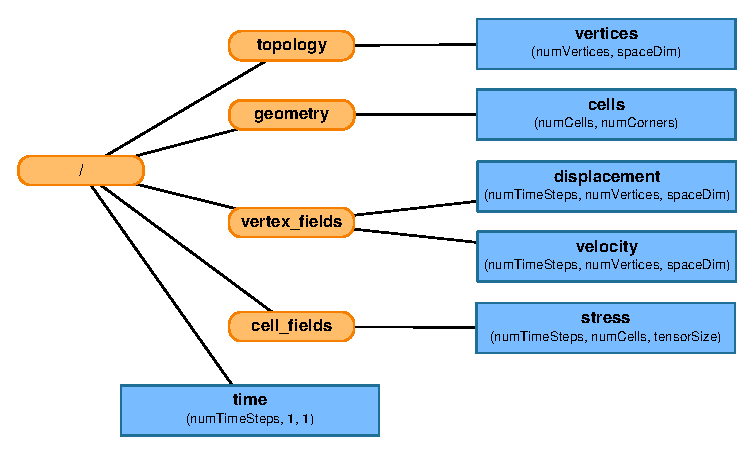
\includegraphics{runpylith/figs/hdf5layout}
\par\end{centering}

\caption{General layout of a PyLith HDF5 file. The orange rectangles with rounded
corners identify the groups and the blue rectangles with sharp corners
identify the datasets. The dimensions of the data sets are shown in
parentheses. Most HDF5 files will contain either \texttt{vertex\_fields}
or \texttt{cell\_fields} but not both. \label{fig:hdf5:layout}}
\end{figure}

\par\end{center}

See Table \ref{tab:material-model-statevars} in Section \ref{sec:material:parameters}
for a table of component values for tensor output in HDF5 files. To
avoid confusion about the ordering of components for tensor data,
we separate the components in the Xdmf file.

HDF5 files do not contain self-correcting features that allow a file
to be read if part of a dataset is corrupted. This type of error can
occur if a job terminates abnormally in the middle or at the end of
a simulation on a large cluster or other parallel machine. Fortunately,
HDF5 also offers the ability to store datasets in external binary
files with the locations specified by links in the HDF5 file. Note
that the use of external data files results in one data file per dataset
in addition to the HDF5 and Xdmf files. The external data files use
the name of the HDF5 file with the dataset name added to the prefix
and the \texttt{.h5} suffix replaced by \texttt{.dat}. The HDF5 files
include relative paths to the external data files, so these files
can also be moved, but they, too, must be kept together in the same
directory. This provides a more robust method of output because one
can generate an HDF5 file associated with the uncorrupted portions
of the external data files should an error occur. Currently, PyLith
does not include a utility to do this, but we plan to add one in a
future release. Thus, there are two options when writing PyLith output
to HDF5 files: (1) including the datasets directly in the HDF5 files
themselves or (2) storing the datasets in external binary files with
just metadata in the HDF5 files. Both methods provide similar performance
because they will use MPI I/O if it is available. 
\begin{quote}
\textbf{\textcolor{red}{Warning:}}\textbf{ }Storing the datasets within
the HDF5 file in a parallel simulation requires that the HDF5 library
be configured with the \texttt{-{}-enable-parallel} option. The binary
PyLith packages include this feature and it is a default setting in
building HDF5 via the PyLith Installer.
\end{quote}
Accessing the datasets for additional analysis or visualization is
nearly identical in the two methods because the use of external data
files is completely transparent to the user except for the presence
of the additional files. Note that in order for ParaView to find the
HDF5 and external data files, it must be run from the same relative
location where the simulation was run. For example, if the simulation
was run from a directory called ``work'' and the HDF5/Xdmf files
were written to ``work/output'', then ParaView should be run from
the ``work'' directory. See Table \ref{tab:material-model-statevars}
in Section \ref{sec:material:parameters} for a table of component
values for tensor output.


\subsubsection{HDF5 Utilities}

HDF5 includes several utilities for examining the contents of HDF5
files. \texttt{h5dump} is very handy for displaying the hierarchy,
dimensions of datasets, attributes, and even the dataset values. 
\begin{quote}
Dump the entire HDF5 file to stdout (not practical or useful for large
files):
\begin{lyxcode}
h5dump~mydata.h5
\end{lyxcode}
Dump the hierarchy of an HDF5 file to stdout:
\begin{lyxcode}
h5dump~-n~mydata.h5
\end{lyxcode}
Dump the hierarchy with dataset dimensions and attributes to stdout:
\begin{lyxcode}
h5dump~-H~mydata.h5
\end{lyxcode}
Dump dataset 'vertices' in group '/geometry' to stdout:
\begin{lyxcode}
h5dump~-d~/geometry/vertices~mydata.h5
\end{lyxcode}
\end{quote}
We have also include a utility \texttt{pylith\_genxdmf} (see Section
\ref{sub:pylith_genxdmf}) that generates an appropriate Xdmf file
from a PyLith HDF5 file. This is very useful if you add fields to
HDF5 files in post-processing and wish to view the results in ParaView
or Visit.


\subsubsection{DataWriterHDF5 Parameters}

This HDF5 writer stores the datasets inside the HDF5 file and the
parameters are:
\begin{description}
\item [{filename}] Name of HDF5 file (the Xdmf filename is generated from
the same prefix).
\end{description}

\subsubsection{DataWriterHDF5Ext Parameters}

This HDF5 writer stores the datasets using external data files (a
more robust method for parallel runs) and the parameters are:
\begin{description}
\item [{filename}] Name of HDF5 file (the external dataset filenames and
the Xdmf filename are generated from the same prefix).
\end{description}
An example of changing the writer from the default VTK writer to the
HDF5 writer with external datasets for output over the domain in a
\texttt{.cfg} file is
\begin{lyxcode}
{[}pylithapp.timedependent.domain.output{]}

output\_freq~=~time\_step

time\_step~=~1.0{*}yr

cell\_data\_fields~=~{[}displacement,velocity{]}

writer~=~pylith.meshio.DataWriterHDF5Ext

writer.filename~=~dislocation.h5
\end{lyxcode}

\section{Tips and Hints\label{sec:Tips:Hints}}


\subsection{Tips and Hints For Running PyLith}
\begin{itemize}
\item Examine the examples for a problem similar to the one you want to
run and dissect it in detail.
\item Start with a uniform-resolution coarse mesh to debug the problem setup.
Increase the resolution as necessary to resolve the solution fields
of interest (resolving stresses/strains may require a higher resolution
than that for resolving displacements).
\item Merge materials using the same material model. This will result in
only one VTK or HDF5 file for each material model rather than several
files.
\item The rate of convergence in quasi-static (implicit) problems can sometimes
be improved by renumbering the vertices in the finite-element mesh
to reduce the bandwidth of the sparse matrix. PyLith can use the reverse
Cuthill-McKee algorithm to reorder the vertices and cells.
\item If you encounter errors or warnings, run \texttt{pylithinfo} or use
the \texttt{-{}-help}, \texttt{-{}-help-components}, and \texttt{-{}-help-properties}
command-line arguments when running PyLith to check the parameters
to make sure PyLith is using the parameters you intended.
\item Use the \texttt{-{}-petsc.log\_}view, \texttt{-{}-petsc.ksp\_monitor},
\texttt{-{}-petsc.ksp\_view}, \texttt{}~\\
\texttt{-{}-petsc.ksp\_converged\_reason}, and \texttt{-{}-petsc.snes\_converged\_reason}
command-line arguments (or set them in a parameter file) to view PyLith
performance and monitor the convergence.
\item Turn on the journals (see the examples) to monitor the progress of
the code.
\end{itemize}

\subsection{Troubleshooting\label{sec:Troubleshooting}}
\begin{itemize}
\item Consult the PyLith FAQ webpage (\url{http://www.geodynamics.org/cig/community/workinggroups/short/workarea/pylith-wiki})
which contains a growing list of common problems and their corresponding
solutions.
\item \texttt{ImportError: liblapack.so.2: cannot open shared object file: No
such file or directory}\end{itemize}
\begin{quote}
PyLith cannot find one of the libraries. You need to set up your environment
variables (e.g., PATH, PYTHONPATH, and LD\_LIBRARY\_PATH) to match
your installation. If you are using the PyLith binary on Linux or
Mac OS X, run the command \texttt{source setup.sh }in the directory
where you unpacked the distribution. This will set up your environment
variables for you. If you are building PyLith from source, please
consult the instructions for building from source.\end{quote}
\begin{itemize}
\begin{singlespace}
\item \texttt{>\textcompwordmark{}> \{command line\}:: }~\\
\texttt{-{}- pyre.inventory(error) }~\\
\texttt{-{}- p4wd <- 'true' }~\\
\texttt{-{}- unrecognized property 'p4wd' }~\\
\texttt{>\textcompwordmark{}> \{command line\}:: }~\\
\texttt{-{}- pyre.inventory(error) }~\\
\texttt{-{}- p4pg <- 'true' }~\\
\texttt{-{}- unrecognized property ' p4pg'}\end{singlespace}
\end{itemize}
\begin{quote}
Verify that the `mpirun' command included in the PyLith package is
the first one on your PATH:

\texttt{\$ which mpirun}

If it is not, adjust your PATH environment variable accordingly.\end{quote}
\begin{itemize}
\item \texttt{\textquotedbl{}merlin.DistributionNotFound: Cheetah\textquotedbl{}
error}\end{itemize}
\begin{quote}
This error occurs when trying to use the 32-bit linux binary on some
64-bit linux systems. One of the Python packages PyLith uses does
not know how to determine the system architecture at runtime. The
workaround is:
\begin{enumerate}
\item Go to the \texttt{lib/python2.7/site-packages} directory.
\item Unzip \texttt{merlin-1.8-py2.7.egg} (if it is a file and not a directory).
\item Go to the merlin directory.
\item Edit \texttt{\_\_init\_\_.py}. Replace line 308 plat = get\_platform()
with plat = \textquotedbl{}linux-i686\textquotedbl{}
\item If \texttt{merlin-1.8-py2.7.egg} is a file, rezip merlin. Go to the
site-packages directory and enter \textquotedbl{}\texttt{zip -r merlin-1.8-py2.7.egg
merlin}\textquotedbl{}.
\end{enumerate}
\end{quote}
\begin{itemize}
\item \texttt{-{}- Solving equations.}~\\
\texttt{{[}0{]}PETSC ERROR: -{}-{}-{}-{}-{}-{}-{}-{}-{}-{}-{}-{}-{}-{}-{}-
Error Message -{}-{}-{}-{}-{}-{}-{}-{}-{}-{}-{}-{}-{}-{}-{}-{}-{}-{}-{}-{}-{}-{}-{}-{}-{}-{}-{}-{}-{}-{}-
}~\\
\texttt{{[}0{]}PETSC ERROR: Detected zero pivot in LU factorization}~\\
\texttt{ see http://www.mcs.anl.gov/petsc/petsc-as/documentation/faq.html\#ZeroPivot!}\end{itemize}
\begin{quote}
This usually occurs when the null space of the system Jacobian is
nonzero, such as the case of a problem without Dirichlet boundary
conditions on any boundary. If this arises when using the split fields
and algebraic multigrid preconditioning, and no additional Dirichlet
boundary conditions are desired, then the workaround is to revert
to using the Additive Schwarz preconditioning without split fields
as discussed in Section \ref{sec:petsc:options}. \end{quote}
\begin{itemize}
\item PyLith crashes with a bus error.\end{itemize}
\begin{quote}
This often indicates that PyLith is using incompatible versions of
libraries. This can result from changing your environment variables
after configuring or installing PyLith (when building from source)
or from errors in setting the environment variables (PATH, LD\_LIBRARY\_PATH,
and PYTHONPATH). If the former case, simply reconfigure and rebuild
PyLith. In the latter case, check your environment variables (order
matters!) to make sure PyLith finds the desired directories before
system directories. \end{quote}
\begin{itemize}
\item PyLith crashes with a segmentation fault.\end{itemize}
\begin{quote}
A segmentation fault might be caused by an error that wasn't trapped
or a bug in the code. Please report these cases so that we can fix
these problems (either trap the error and provide the user with an
informative error message, or fix the bug). If this occurs with any
of the problems distributed with PyLith, simply submit a bug report
(see Section \ref{sec:Getting-Help-and}) indicating which problem
you ran and your platform. If the crash occurs for a problem you created,
it is a great help if you can try to reproduce the crash with a very
simple problem (e.g., adjust the boundary conditions or other parameters
of one of the examples to reproduce the segmentation fault). Submit
a bug report along with log files showing the backtrace from a debugger
(e.g., gdb) and the valgrind log file (only available on Linux platforms).
You can generate a backtrace using the debugger by using the \texttt{-{}-petsc.start\_in\_debugger}
command-line argument:\end{quote}
\begin{lyxcode}
pylith~{[}..args..{]}~-{}-petsc.start\_in\_debugger

(gdb)~continue

(gdb)~backtrace\end{lyxcode}
\begin{quote}
To use valgrind to detect the memory error, first go to your working
directory and run the problem with \texttt{-{}-launcher.dry}:\end{quote}
\begin{lyxcode}
pylith~{[}..args..{]}~-{}-launcher.dry\end{lyxcode}
\begin{quote}
Instead of actually running the problem, this causes PyLith to dump
the mpirun/mpiexec command it will execute. Copy and paste this command
into your shell so you can run it directly. Insert the full path to
valgrind before the full path to mpinemesis and tell valgrind to use
a log file:\end{quote}
\begin{lyxcode}
{\footnotesize{}mpirun~-np~1~/path/to/valgrind~-{}-log-file=valgrind-log~~/path/to/mpinemesis~-{}-pyre-start~{[}..lots~of~junk..{]}}{\footnotesize \par}
\end{lyxcode}

\section{Post-Processing Utilities}

The PyLith distribution includes a few post-processing utilities.
These are Python scripts that are installed into the same bin directory
as the \texttt{pylith} executable.


\subsection{\texttt{pylith\_eqinfo}}

This utility computes the moment magnitude, seismic moment, seismic
potency, and average slip at user-specified time snapshots from PyLith
fault HDF5 output. The utility works with output from simulations
with either prescribed slip and/or spontaneous rupture. Currently,
we compute the shear modulus from a user-specified spatial database
at the centroid of the fault cells. In the future we plan to account
for lateral variations in shear modulus across the fault when calculating
the seismic moment. The Python script is a Pyre application, so its
parameters can be specified using \texttt{.cfg} and command line arguments
just like PyLith. The Pyre properties and facilities include:
\begin{description}
\item [{output\_filename}] Filename for output of slip information.
\item [{faults}] Array of fault names.
\item [{filename\_pattern}] Filename pattern in C/Python format for creating
filename for each fault. Default is\\
\texttt{output/fault\_\%s.h5}.
\item [{snapshots}] Array of timestamps for slip snapshosts ({[}-1{]} means
use last time step in file, which is the default).
\item [{snapshot\_units}] Units for timestamps in array of snapshots.
\item [{db\_properties}] Spatial database for elastic properties.
\item [{coordsys}] Coordinate system associated with mesh in simulation.
\end{description}

\subsection{\texttt{\label{sub:pylith_genxdmf}pylith\_genxdmf}}

This utility generates Xdmf files from HDF5 files that conform to
the layout used by PyLith. It is a simple Python script with a single
command line argument, the HDF5 file for input. Typically, it is sued
to regenerate Xdmf files that get corrupted or lost due to renaming
and moving. It is also useful in updating Xdmf files when users add
fields to HDF5 files during post-processing.
\begin{lyxcode}
pylith\_genxdmf~-{}-file=\textit{PYLITH\_HDF5\_FILE}\end{lyxcode}
\begin{quote}
\textbf{\textcolor{red}{Warning:}}\textbf{ }If the HDF5 files contain
external datasets, then this utility should be run from the same relative
path to the HDF5 files as when they were created. For example, if
a PyLith simulation was run from directory \texttt{work} and HDF5
files were generated in \texttt{output/work}, then the utility should
be run from the directory \texttt{work}. Furthermore, a visualization
tool, such as ParaView, should also be started from the working directory
\texttt{work}.\end{quote}


\chapter{Tutorials}

\section{Overview}

Each tutorial is a self-contained lesson in how to use PyLith. The
tutorials increase in degree of complexity from one to the next. 

\subsection{Prerequisites}

Before you begin any of the tutorials, you will need to install PyLith
following the instructions in section~\ref{sec:install}. In order to
work through a full tutorial, in addition to \application{PyLith} you
will need \href{http://www.hpfem.jku.at/netgen/}{\application{NETGEN}}
to generate the mesh and \href{http://www.paraview.org}{ParaView} to
view simulation results. You may use other packages, but some adaption
from what is described here will be necessary. Alternatively, you can
just complete a subset of the tutorial using files provided (as
described below), skipping the steps for which you do not have the
proper software packages installed.

The files needed to work through the tutorials have been collected
into a single tarball. Each tutorial contains instructions for
downloading and unpacking the tutorial tarball.

\subsection{Tutor}

Each tutorial includes a simple Python script, \filename{tutor.py}, to
help with miscellaneous tasks, such as copying provided files into a
working directory. This script can (1) check to make sure the files
necessary for a given step in the tutorial exist, (2) retrieve any
missing files from the tutorial archive directory that are needed for
a given step, or (3) prepare the work area for a given step by
removing old files that would otherwise be overwritten. You can run
\command{tutor.py} with the \option{-h} option for more
information. We will use this script at the beginning of each step of
the tutorials to retrieve files as necessary from the tutorial archive
directory.

\begin{tip}
  When retrieving files from the archive directory, \command{tutor.py}
  will not overwrite files that already exist in the workarea
  directory. This means that if you mangle files in the working area,
  you should remove them and let the tutor retrieve clean copies.
\end{tip}

\section{Tutorial For Simple Strike-Slip Fault}

\subsection{Overview}

In this tutorial we will walk through the steps necessary to
construct, run, and view the results of a benchmark problem involving
a simple, vertical, through-going strike-slip fault. This problem
examines the elastic deformation from a single, finite, right-lateral
earthquake in 3-D without body forces.

\subsection{Problem Description}

The model domain is a cube with edges 1 km long (0 km $\leq$ x $\leq$
1 km; 0 km $\leq$ y $\leq$ 1 km; 0 km $\leq$ z $\leq$ 1 km) and is
composed of two materials. The fault separates two materials that have
the same properties. Both materials are Poisson solids with Lame's
constants ($\mu$ and $\lambda$) equal to 30 GPa.

The strike-slip fault dips at an angle of 90 degrees. The slip
distribution is 1.0 m of uniform right-lateral motion.

The plane y=0 is a plane of symmetry, so the y-DOF displacements on
this face are zero. The other lateral faces and bottom of the mesh are
traction-free.

\begin{figure}
  \begin{center}
    %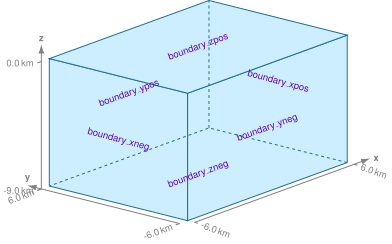
\includegraphics{figs/geometry}
    \caption{Geometry of model domain for simple model with strike-slip fault.}
  \end{center}
\end{figure}  

\subsubsection{Workflow}

The complete workflow used to create the input files for this tutorial
is shown in figure~\ref{fig:splittest:workflow}. 

\begin{figure}[htbp]
  \begin{center}
    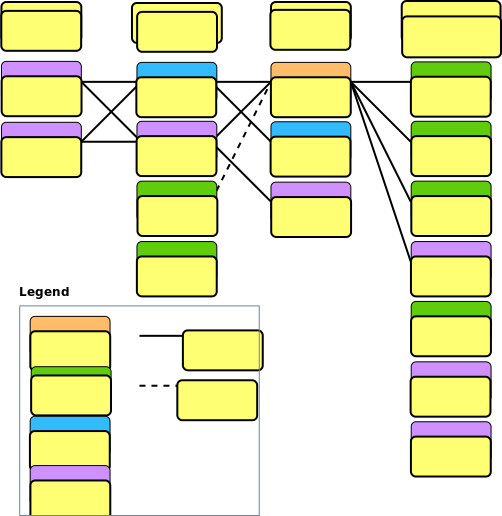
\includegraphics{figs/workflow}
    \caption{Workflow for setting up input files for example with
      simple strike-slip faylt.}
    \label{fig:splittest:workflow}
  \end{center}
\end{figure}

\subsection{Download and unpack}

We will start by downloading the tutorial tarball and unpacking it.

\begin{enumerate}
\item Download the \href{http://www.geodynamics.org:8080/cig/Members/willic3/pylithusers/pylith0.8/pylith-0.8\_tutorials.tgz}{tutorial tarball}
  and unpack it in a location of your choosing.

  \begin{screen}
    \shellprompt\userinput{tar -zxvf pylith-0.8\_tutorials.tgz}
  \end{screen}
  
\item Go to the \directory{tutorials/splittest} directory.
  The \directory{archive} directory contains all of the input and
  output files associated with this tutorial. We will copy input files
  from this directory into the \directory{workarea} directory. At each
  step, you can check to make sure your input and output agree with
  the files in the \directory{archive} directory. These files also
  allow you to start at an intermediate step as described in the next
  section.

  \begin{screen}
    \shellprompt\userinput{cd tutorials/splittest}
  \end{screen}

\end{enumerate}

\subsection{Tutor}

Copy the \filename{tutor.py} script from the \directory{archive}
directory into the \directory{workarea} directory. 

\begin{tip}
  If you have run this tutorial previously, you may want to run
  \command{tutor.py} in mode "clean" with step "all" to clear out all
  old tutorial files.
\end{tip}

\begin{screen}
\shellprompt\userinput{cd workarea}
\shellprompt\userinput{cp ../archive/tutor.py .}
\shellprompt\userinput{./tutor.py -m clean -s all}
\end{screen}

\subsection{Generate the mesh}

In this step we will generate the finite-element mesh for the
benchmark problem using \application{NETGEN}.

\begin{enumerate}
\item In the \directory{splittest/workarea} directory, run
  \command{tutor.py} for step "mesh" with mode "retrieve" to fetch the
  geometry file for \application{NETGEN}. You may also want to run
  \command{tutor.py} for this step with mode "clean" to clean out old
  files.

  \begin{screen}
    \shellprompt\userinput{./tutor.py -m retrieve -s mesh}
    \shellprompt\userinput{./tutor.py -m clean -s mesh}
  \end{screen}
  
\item Examine the \filename{splittest.geo} file to see how the geometry
  for the problem is defined. Notice that the fault plan has
  been flagged with a boundary condition code. This will be
  used to associate boundary conditions with the fault surface and the
  associated nodes. We do not have to flag the lateral faces and top
  and bottom of the mesh because they are traction-free, which is a
  natural boundary condition in the finite-element formulation.
\item Start up \application{NETGEN} by running \command{ng}.

  \begin{screen}
    \shellprompt\userinput{ng}
  \end{screen}
  
\item Select \guimenu{File}\guiselect\guimenuitem{Load Geometry}
  and select \filename{splittest.geo}.
\item Click on \guibutton{Generate Mesh}.
\item Export the mesh to a file named \filename{splittest.netgen},
  making sure the export filetype is "Neutral format".
\item You can now exit \application{NETGEN}.
\end{enumerate}

\subsection{Setup simulation input files}

In this step we will setup the PyLith input files for the mesh and
boundary conditions.

\begin{enumerate}
\item Run \command{tutor.py} for step "setup" with mode "retrieve" to
  fetch files from the archive.

  \begin{screen}
    \shellprompt\userinput{./tutor.py -m retrieve -s setup}
  \end{screen}
  
\item We will use a simple Fortran utility to generate PyLith
  input files from the \application{NETGEN} output.

  \begin{description}
  \item[\command{readnetgen}] A Fortran program to read
    \application{NETGEN} neutral format and create several of the
    input files needed by PyLith.
  \end{description}
  
\item Run the \command{readnetgen} utility program to process the
  \application{NETGEN} output file into PyLith compatible input files.
  It will ask for a root filename, enter \filename{splittest}. This
  utilitiy will generate the following files:
  \filename{splittest.w01.wink}, \filename{splittest.coord},
  \filename{splittest.connect}, \filename{splittest.bc},
  \filename{splittest.1.fcoord}, \filename{splittest.1.fbc}.

  \begin{screen}
    \shellprompt\userinput{../../utils/readnetgen}
    \prompt{\ Enter root name for all files.  Both input and}
    \prompt{\ output files will all have this prefix:}
    \userinput{splittest}
  \end{screen}
  
\item The boundary conditions on the fault for this example are
  very simple. As a result, the \filename{splittest.split} file was
  generated by hand. You should examine this file to see how a uniform
  right-lateral slip of 1.0 m is applied to the fault surface.

  \begin{warning}
    If you make any changes to \filename{splittest.geo} or change the
    geometry within \application{NETGEN}, the split-node file
    \filename{splittest.split} will no longer be correct and you will
    have to generate one yourself.  Note that it is also possible that
    a different version of \application{NETGEN} may provide a slightly
    different mesh, which would also be incompatible with the provided
    boundary conditions.
  \end{warning}
  
\item The external boundary conditions for this benchmark simply
  involve ... ADD STUFF HERE.

  \begin{warning}
    If you make any changes to \filename{splittest.geo} or change the
    geometry within \application{NETGEN}, the boundary condition file
    \filename{splittest.bc} will no longer be correct and you will
    have to generate one yourself.  Note that it is also possible that
    a different version of \application{NETGEN} may provide a slightly
    different mesh, which would also be incompatible with the provided
    boundary conditions.
  \end{warning}
\end{enumerate}

\subsection{Run the simulation on one processor}

In this step we will run the simulation on a single processor.

\begin{enumerate}
\item Run \command{tutor.py} for step "run1" with mode "retrieve" to
  fetch some parameter files from the archive.

  \begin{screen}
    \shellprompt\userinput{./tutor.py -m retrieve -s run1}
  \end{screen}
  
\item In \filename{splittest.fuldat}, we have specified that we want
  full output at time steps 10, 50, and 100. We define two materials
  with elastic behavior in
  \filename{splittest.prop}. In \filename{splittest.statevar} we choose to
  include total stress, total strain, incremental stress, and
  incremental strain in the output. As defined in
  \filename{splittest.time}, the simulation will have 100 time steps of
  0.1 year each.
\item Run the simulation by executing \userinput{runbm.py -n 1}, where
  the 1 refers to the number of processors.

  \begin{tip}
    All of the input is echoed in the file \filename{splittest.ascii}.
    You can check to make sure your input is digested correctly by
    examining this file. For large problems, this file can be quite
    large. You can suppress creation of this file using the command
    line argument \option{--scanner.asciiOutput=none} flag. On the
    other hand, for debugging purposes in small problems, you may wish
    to output everything, including the computed results, in this file
    using \option{--scanner.asciiOutput=full}.
  \end{tip}
  
  \begin{screen}
    \shellprompt\userinput{./runbm.py -n 1}
  \end{screen}
\end{enumerate}

\subsection{Visualize the single processor run}

Now it is time to visualize the results of the simulation. By default,
PyLith writes simulation output using \href{http://help.avs.com/Express/doc/help/reference/dvmac/UCD\_Form.htm}{\application{AVS} UCD
  files}.
These can be read by several other visualization tools besides
\application{AVS}, e.g., \application{ParaView} and \application{Iris
  Explorer}. We will use the open-source application
\application{ParaView} to visualize the results.
    
\begin{enumerate}
\item If necessary, run \command{tutor.py} for step "viz1" with mode
  "retrieve" to fetch the simulation output from the archive.

  \begin{screen}
    \shellprompt\userinput{./tutor.py -m retrieve -s viz1}
  \end{screen}
  
\item PyLith does not write complete UCD files. So the first step is
  to combine the mesh topology information with the output at a given
  time step into a complete UCD file. For example, use \command{cat}
  to merge the nodal coordinates file
  (\filename{splittest\_1.0.mesh.inp}) and the nodal displacements at
  time step 10 file (\filename{splittest\_1.0.mesh.time.00010.inp}) into
  \filename{splittest\_1.0.mesh.t00010.inp}.

  \begin{screen}
    \shellprompt\userinput{cat splittest\_1.0.mesh.inp splittest\_1.0.mesh.time.00010.inp \(\backslash\)}
    \userinput{> splittest\_1.0.mesh.t00010.inp}
\end{screen}

\item Start \application{ParaView} by executing \command{paraview}.

  \begin{screen}
    \shellprompt\userinput{paraview}
  \end{screen}
  
\item Load the UCD file that you just created by selecting
  \guimenu{File}\guiselect\guimenuitem{Open Data}. Select the file in
  the dialog box and the click the \guibutton{Open} button. Click the
  \guibutton{Accept} button. You should see a color rendering of the x
  displacements. You can use the mouse to rotate, translate, and zoom.
  Your image should look similar to the one in
  figure~\ref{fig::splittest:xdisp:t10}.
        
  \begin{figure}[htbp]
    \begin{center}
      %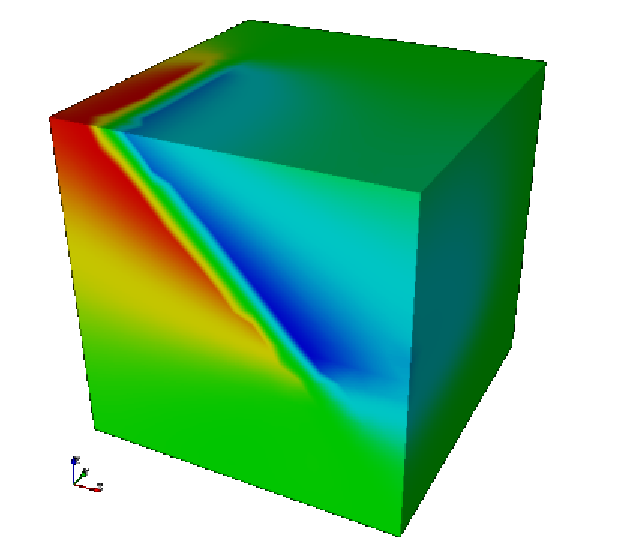
\includegraphics{figs/xdisp_t10}
      \caption{ParaView rendering of displacement in x-direction at
          time step 10 (10 yrs after imposed dislocation) for the
          simple strike-slip example.}
      \label{fig:splittest:xdisp:t10}
    \end{center}
  \end{figure}
  
\item In the \guibutton{Display} tab, you can change several options,
  such as including a color bar, coloring a different component,
  interpolating colors, and changing the color map.
\item Let's show the displacements as vectors. Click on the calculator
  icon, and add the three displacement components together. Enter
  \begin{screen}
  XDispl*iHat + YDispl*jHat + ZDispl*kHat
  \end{screen}
  in the \guimenuitem{Calculator}
  box. Note the variable names are available by clicking on the
  \guibutton{scalars} button and the \guibutton{iHat},
  \guibutton{jHat}, \guibutton{kHat} buttons are on the right side of
  the top row. Click on the \guibutton{Accept} button. To show the
  dataset as vectors, click on the \guibutton{glyph} button (looks
  like several dots) in the toolbar. After clicking the
  \guibutton{Accept} button, you should have a vector plot. You can
  turn on/off other datasets by clicking on the eye icon to the left
  of the dataset name. If you color the surfaces using the
  x-displacements field while also making the displacement vectors
  visible (colored using property), you should see an image similar to
  the one in figure~\ref{fig:splittest:xdisp:vec:t10}.

  \begin{figure}[htbp]
    \begin{center}
      %\includegraphics{figs/splittest_xdisp_vec_t10}
      \caption{ParaView rendering of displacement in x-direction and
        displacement vectors at time step 10 (10 yrs after imposed
        dislocation) for the simple strike-slip example.}
      \label{fig:splittest:xdisp:vec:t10}
    \end{center}
  \end{figure}      

\end{enumerate}

\subsection{Run the simulation on two processors}

In this step we will run the simulation on two processors. Even if
your machine only has one processor, a "multprocessor" job will run as
multiple processes on the single processor. In such cases, the job
will run slightly slower than the single processor run, but the two
processes will behave independently as if they are on different
processors.

\begin{enumerate}
\item Run \command{tutor.py} for step "run2" with mode "retrieve" to
  make sure all parameter files are available.

  \begin{screen}
    \shellprompt\userinput{./tutor.py -m retrieve -s run2}
  \end{screen}
  
\item The parameter files are the same as those in the single
  processor run. The \command{runbm} script will automatically take
  care of duplicating these files so that there is one for each
  processor.
\item Run the simulation by executing \command{runbm.py -n 2}, where
  the 2 refers to the number of processors.

  \begin{screen}
    \shellprompt\userinput{./runbm.py -n 2}
  \end{screen}
\end{enumerate}

\subsection{Visualize the two processor run}

PyLith does not currently support parallel output, so each processor
writes its UCD output to a different file. This means that you need to
form complete UCD files for each processor and then load each one into
\application{ParaView}.

\begin{enumerate}
\item If necessary, run \command{tutor.py} for step "viz2" with mode
  "retrieve" to fetch the simulation output from the archive.

  \begin{screen}
    \shellprompt\userinput{./tutor.py -m retrieve -s viz2}
  \end{screen}
  
\item As in the case of the single processor run, the first step is to
  combine the mesh topology information with the output at a given
  time step into a complete UCD file. Because PyLith writes the output
  from each processor into a different file, we must run \command{cat}
  twice to create UCD files for each processor.

  \begin{screen}
    \shellprompt\userinput{cat splittest\_2.0.mesh.inp splittest\_2.0.mesh.time.00010.inp \(\backslash\)}
      \userinput{> splittest\_2.0.mesh.t00010.inp}
    \shellprompt\userinput{cat splittest\_2.1.mesh.inp splittest\_2.1.mesh.time.00010.inp \(\backslash\)}
      \userinput{> splittest\_2.1.mesh.t00010.inp}
  \end{screen}

\item Start \application{ParaView} by executing \command{paraview}.

  \begin{screen}
    \shellprompt\userinput{paraview}
  \end{screen}
  
\item Load the UCD files that you just created by selecting
  \guimenu{File}\guiselect\guimenuitem{Open Data}. Select the file in
  the dialog box and the click the \guibutton{Open} button. Click the
  \guibutton{Accept} button. You can now visualize the datasets just
  like you did for the single processor case.
\item You can merge the datasets from the different processors by
  selecting \guimenu{Filter}\guiselect\guimenuitem{Append}. Doing so
  will allow you to operate on the data from all of the processors
  simultaneously instead of having to repeat any processing for every
  processor.
\end{enumerate}

\section{Tutorial Using Reverse-Slip Without Gravity Benchmark}

\subsection{Overview}

In this tutorial, we will walk through the steps necessary to
construct, run, and view the results of a benchmark problem involving
reverse slip on a dipping fault. This problem examines the
viscoelastic (Maxwell) relaxation of stress from a single, finite,
reverse-slip earthquake in 3-D without body forces.


\subsection{Problem Description}

The model domain is a cube with edges 24 km long (0 km $\leq$ x $\leq$
24 km; 0 km $\leq$ y $\leq$ 24 km; -24 km $\leq$ z $\leq$ 0) and
is composed of two materials. One material occupies the top-half of
the domain, -12 km $\leq$ z $\leq$ 0 km, while the other occupies
the lower half, -24 km $\leq$ z $<$ 12 km. Both materials are Poisson
solids with Lame's constants ($\mu$ and $\lambda$) equal to 30 GPa and
Maxwell viscoelastic properties. The top layer has a viscosity of
$10^25$ Pa-s (and is essentially elastic) while the bottom layer has a
viscosity of $10^18$ Pa-s.

The reverse fault dips at an angle of 45 degrees. The top of the fault
sits at x = 4 km with the bottom of the fault at x = 20 km. The fault
surface is confined to the region 0 km $\leq$ y $\leq$ 16 km and -16
km $\leq$ z $\leq$ 0 km. The slip distribution is 1.0 m of uniform
thrust motion for -12 km $\leq$ z with a linear taper to 0 at z = -16
km.

The plane y=0 is a plane of symmetry, so the y-DOF displacements on
this face are zero. The boundary conditions on the other lateral faces
and bottom of the mesh are the displacements from the analytical
elastic solution. These displacements are held fixed through time.

\begin{figure}
  \begin{center}
    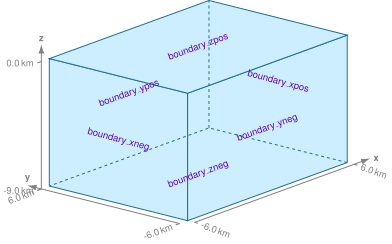
\includegraphics{figs/geometry}
    \caption{Geometry of model domain for reverse-slip benchmark.}
  \end{center}
\end{figure}  

\subsubsection{Workflow}

The complete workflow used to create the input files for this tutorial
is shown in figure~\ref{fig:bmrsnog:workflow}. Because some of the
steps involve commercial software (e.g., Matlab), we will skip those
steps in this tutorial.

\begin{figure}[htbp]
  \begin{center}
    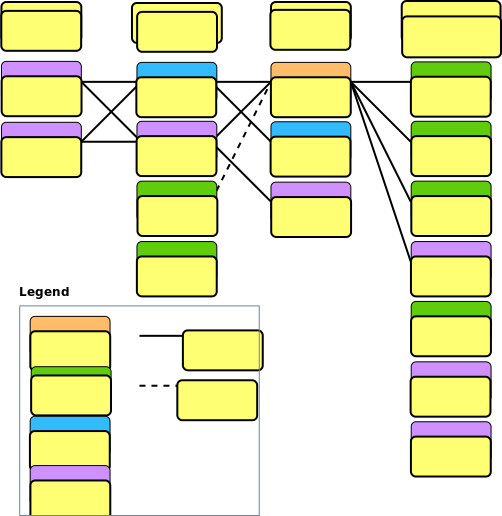
\includegraphics{figs/workflow}
    \caption{Workflow for setting up input files for benchmark with reverse
      slip and no gravity.}
    \label{fig:bmrsnog:workflow}
  \end{center}
\end{figure}

\subsection{Download and unpack}

We will start by downloading the tutorial tarball and unpacking it.

\begin{enumerate}
\item Download the \link{tutorial
    tarball}{http://www.geodynamics.org:8080/cig/Members/willic3/pylithusers/pylith0.8/pylith-0.8\_tutorials.tgz}
  and unpack it in a location of your choosing.

  \begin{screen}
    \shellprompt\userinput{tar -zxvf pylith-0.8\_tutorials.tgz}
  \end{screen}
  
\item Go to the \directory{tutorials/reversenog} directory.
  The \directory{archive} directory contains all of the input and
  output files associated with this tutorial. We will copy input files
  from this directory into the \directory{workarea} directory. At each
  step, you can check to make sure your input and output agree with
  the files in the \directory{archive} directory. These files also
  allow you to start at an intermediate step as described in the next
  section.

  \begin{screen}
    \shellprompt\userinput{cd tutorials/reversenog}
  \end{screen}

\end{enumerate}

\subsection{Tutor}

Copy the \filename{tutor.py} script from the \directory{archive}
directory into the \directory{workarea} directory. 

\begin{tip}
  If you have run this tutorial previously, you may want to run
  \command{tutor.py} in mode "clean" with step "all" to clear out all
  old tutorial files.
\end{tip}

\begin{screen}
\shellprompt\userinput{cd workarea}
\shellprompt\userinput{cp ../archive/tutor.py .}
\shellprompt\userinput{./tutor.py -m clean -s all}
\end{screen}

\subsection{Generate the mesh}

In this step we will generate the finite-element mesh for the
benchmark problem using \application{NETGEN}.

\begin{enumerate}
\item In the \directory{reversenog/workarea} directory, run
  \command{tutor.py} for step "mesh" with mode "retrieve" to fetch the
  geometry file for \application{NETGEN}. You may also want to run
  \command{tutor.py} for this step with mode "clean" to clean out old
  files.

  \begin{screen}
    \shellprompt\userinput{./tutor.py -m retrieve -s mesh}
    \shellprompt\userinput{./tutor.py -m clean -s mesh}
  \end{screen}
  
\item Examine the \filename{bmrsnog.geo} file to see how the geometry
  for the problem is defined. Notice that the different planes have
  been flagged with different boundary condition codes. These will be
  used to associate boundary conditions with surfaces and element
  nodes.
\item Start up \application{NETGEN} by running \command{ng}.

  \begin{screen}
    \shellprompt\userinput{ng}
  \end{screen}
  
\item Select \guimenu{File}\guiselect\guimenuitem{Load Geometry}
  and select \filename{bmrsnog.geo}.
\item Click on \guibutton{Generate Mesh}.
\item Export the mesh to a file named \filename{bmrsnog.netgen},
  making sure the export filetype is "Neutral format".
\item You can now exit \application{NETGEN}.
\end{enumerate}

\subsection{Setup simulation input files}

In this step we will setup the PyLith input files for the mesh and
boundary conditions.

\begin{enumerate}
\item Run \command{tutor.py} for step "setup" with mode "retrieve" to
  fetch files from the archive.

  \begin{screen}
    \shellprompt\userinput{./tutor.py -m retrieve -s setup}
  \end{screen}
  
\item We will use two simple Fortran utilities to generate PyLith
  input files from the \application{NETGEN} output.

  \begin{description}
  \item[\command{readnetgen}] A Fortran program to read
    \application{NETGEN} neutral format and create several of the
    input files needed by PyLith.
  \item[\command{faultcalc}] A Fortran program to compute split node
    displacements using second order polynomials over specified
    regions.
  \end{description}
  
\item Run the \command{readnetgen} utility program to process the
  \application{NETGEN} output file into PyLith compatible input files.
  It will ask for a root filename, enter \filename{bmrsnog}. This
  utilitiy will generate the following files:
  \filename{bmrsnog.w01.wink}, \filename{bmrsnog.coord},
  \filename{bmrsnog.connect}, \filename{bmrsnog.bc},
  \filename{bmrsnog.1.fcoord}, \filename{bmrsnog.1.fbc}.

  \begin{screen}
    \shellprompt\userinput{../../utils/readnetgen}
    \prompt{~Enter root name for all files.  Both input and}\\
    \prompt{~output files will all have this prefix:}\\
    \userinput{bmrsnog}
  \end{screen}
  
\item The boundary conditions on the fault for this benchmark are
  somewhat complex. The utility program \command{faultcalc} creates
  split node boundary conditions over specified regions, using
  functions based on second degree polynomials. The
  \command{readnetgen} program has already produced the main input for
  \command{faultcalc} -- split node definitions in
  \filename{bmrsnog.1.fbc} and nodal coordinates in
  \filename{bmrsnog.coord}. The file \filename{bmrsnog.fault.par}
  contains the polynomial coefficients for this benchmark problem. Run
  \command{faultcalc} to get the \filename{bmrsnog.split} file that
  PyLith needs as input.

  \begin{screen}
    \shellprompt\userinput{../../utils/faultcalc p=bmrsnog.fault.par n=bmrsnog.coord\\
      i=bmrsnog.1.fbc o=bmrsnog.split}
  \end{screen}
  
\item The external boundary conditions for this benchmark are also
  complicated and require computing the displacements for the
  analytical elastic solution at each finite element node on the
  external boundaries. The file specifying these boundary conditions,
  \filename{bmrsnog.bc}, was produced with \command{readnetgen} using
  the \filename{bmrsnog.aux} file (which contains precomputed
  displacements for the external boundaries for the mesh produced from
  the \filename{bmrsnog.geo} geometry).

  \begin{warning}
    If you make any changes to \filename{bmrsnog.geo} or change the
    geometry within \application{NETGEN}, the boundary condition file
    \filename{bmrsnog.bc} will no longer be correct and you will have
    to generate one yourself.  Note that it is also possible that a
    different version of \application{NETGEN} may provide a slightly
    different mesh, which would also be incompatible with the provided
    boundary conditions.
  \end{warning}
\end{enumerate}

\subsection{Run the simulation on one processor}

In this step we will run the simulation on a single processor.

\begin{enumerate}
\item Run \command{tutor.py} for step "run1" with mode "retrieve" to
  fetch some parameter files from the archive.

  \begin{screen}
    \shellprompt\userinput{./tutor.py -m retrieve -s run1}
  \end{screen}
  
\item In \filename{bmrsnog.fuldat}, we have specified that we want
  full output at time steps 10, 50, and 100. We define six materials
  with both elastic and viscoelastic behavior in
  \filename{bmrsnog.prop}. In \filename{bmrsnog.statevar} we choose to
  include total stress, total strain, incremental stress, and
  incremental strain in the output. As defined in
  \filename{bmrsnog.time}, the simulation will have 100 time steps of
  0.1 year each.
\item Run the simulation by executing \userinput{runbm.py -n 1}, where
  the 1 refers to the number of processors.

  \begin{tip}
    All of the input is echoed in the file \filename{bmrsnog.ascii}.
    You can check to make sure your input is digested correctly by
    examining this file. For large problems, this file can be quite
    large. You can suppress creation of this file using the command
    line argument \option{--scanner.asciiOutput=none} flag. On the
    other hand, for debugging purposes in small problems, you may wish
    to output everything, including the computed results, in this file
    using \option{--scanner.asciiOutput=full}.
  \end{tip}
  
  \begin{screen}
    \shellprompt\userinput{./runbm.py -n 1}
  \end{screen}
\end{enumerate}

\subsection{Visualize the single processor run}

Now it is time to visualize the results of the simulation. By default,
PyLith writes simulation output using \link{\application{AVS} UCD
  files}{http://help.avs.com/Express/doc/help/reference/dvmac/UCD\_Form.htm}.
These can be read by several other visualization tools besides
\application{AVS}, e.g., \application{ParaView} and \application{Iris
  Explorer}. We will use the open-source application
\application{ParaView} to visualize the results.
    
\begin{enumerate}
\item If necessary, run \command{tutor.py} for step "viz1" with mode
  "retrieve" to fetch the simulation output from the archive.

  \begin{screen}
    \shellprompt\userinput{./tutor.py -m retrieve -s viz1}
  \end{screen}
  
\item PyLith does not write complete UCD files. So the first step is
  to combine the mesh topology information with the output at a given
  time step into a complete UCD file. For example, use \command{cat}
  to merge the nodal coordinates file
  (\filename{bmrsnog\_1.0.mesh.inp}) and the nodal displacements at
  time step 10 file (\filename{bmrsnog\_1.0.mesh.time.00010.inp}) into
  \filename{bmrsnog\_1.0.mesh.t00010.inp}.

  \begin{screen}
    \shellprompt\userinput{cat bmrsnog\_1.0.mesh.inp bmrsnog\_1.0.mesh.time.00010.inp \ \\
> bmrsnog\_1.0.mesh.t00010.inp}
\end{screen}

\item Start \application{ParaView} by executing \command{paraview}.

  \begin{screen}
    \shellprompt\userinput{paraview}
  \end{screen}
  
\item Load the UCD file that you just created by selecting
  \guimenu{File}\guiselect\guimenuitem{Open Data}. Select the file in
  the dialog box and the click the \guibutton{Open} button. Click the
  \guibutton{Accept} button. You should see a color rendering of the x
  displacements. You can use the mouse to rotate, translate, and zoom.
  Your image should look similar to the one in
  figure~\ref{fig::bmrsnog:xdisp:t10}.
        
  \begin{figure}[htbp]
    \begin{center}
      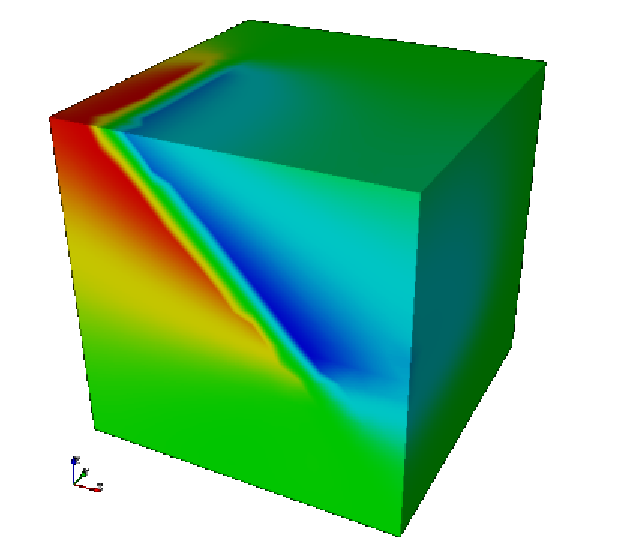
\includegraphics{figs/xdisp_t10}
      \caption{ParaView rendering of displacement in x-direction at
          time step 10 (10 yrs after imposed dislocation) for the
          reverse slip without gravity benchmark.}
      \label{fig:bmrsnog:xdisp:t10}
    \end{center}
  \end{figure}
  
\item In the \guibutton{Display} tab, you can change several options,
  such as including a color bar, coloring a different component,
  interpolating colors, and changing the color map.
\item Let's show the displacements as vectors. Click on the calculator
  icon, and add the three displacement components together. Enter
  "XDispl*iHat+YDispl*jHat+ZDispl*kHat" in the \guimenuitem{Calculator}
  box. Note the variable names are available by clicking on the
  \guibutton{scalars} button and the \guibutton{iHat},
  \guibutton{jHat}, \guibutton{kHat} buttons are on the right side of
  the top row. Click on the \guibutton{Accept} button. To show the
  dataset as vectors, click on the \guibutton{glyph} button (looks
  like several dots) in the toolbar. After clicking the
  \guibutton{Accept} button, you should have a vector plot. You can
  turn on/off other datasets by clicking on the eye icon to the left
  of the dataset name. If you color the surfaces using the
  x-displacements field while also making the displacement vectors
  visible (colored using property), you should see an image similar to
  the one in figure~\ref{fig:bmrsnog:xdisp:vec:t10}.

  \begin{figure}[htbp]
    \begin{center}
      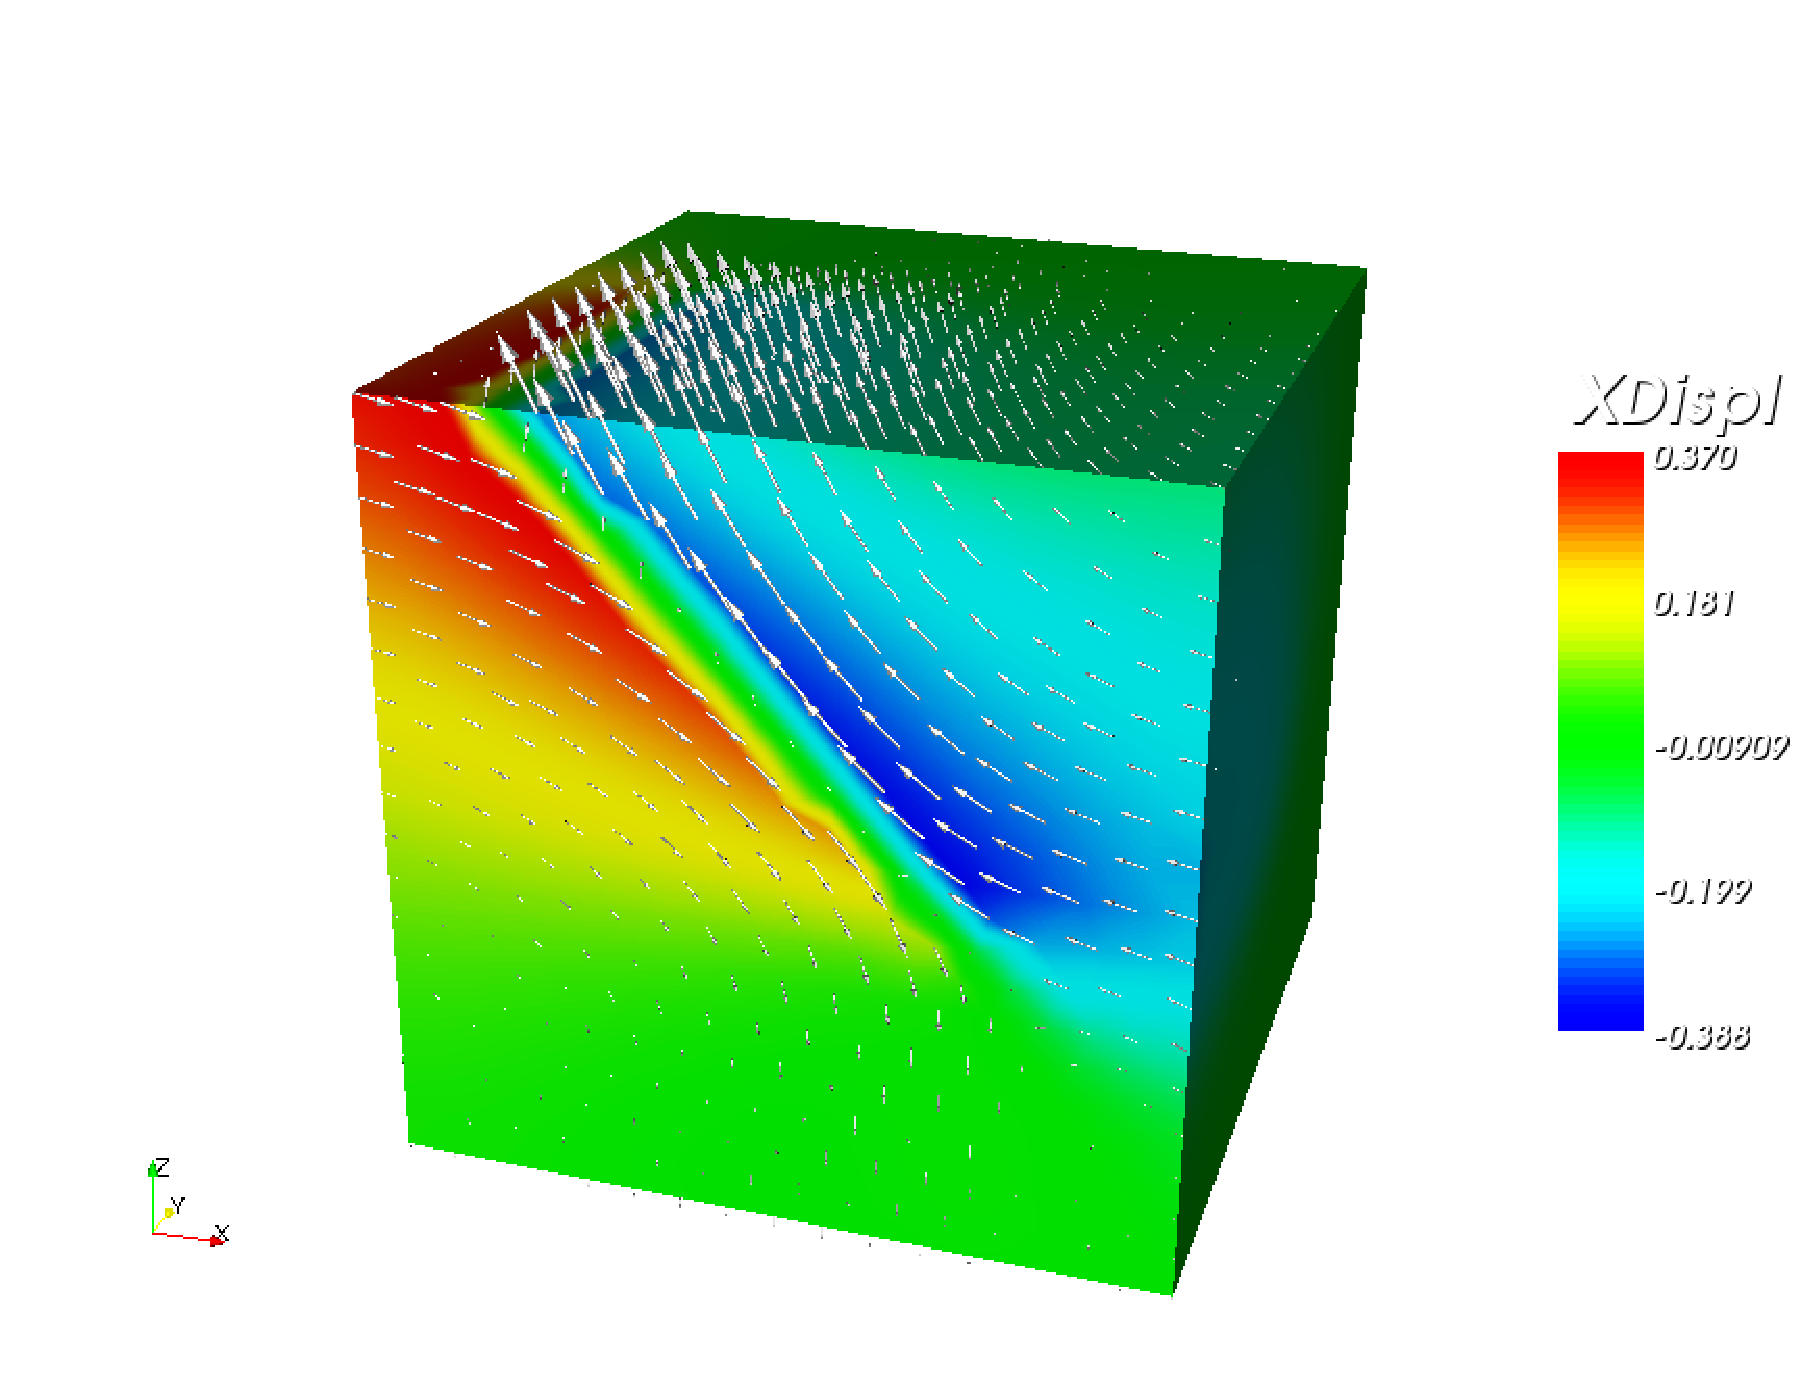
\includegraphics{figs/xdisp_vec_t10}
      \caption{ParaView rendering of displacement in x-direction and
        displacement vectors at time step 10 (10 yrs after imposed
        dislocation) for the reverse slip without gravity
        benchmark.}
      \label{fig:bmrsnog:xdisp:vec:t10}
    \end{center}
  \end{figure}      

\end{enumerate}

\subsection{Run the simulation on two processors}

In this step we will run the simulation on two processors. Even if
your machine only has one processor, a "multprocessor" job will run as
multiple processes on the single processor. In such cases, the job
will run slightly slower than the single processor run, but the two
processes will behave independently as if they are on different
processors.

\begin{enumerate}
\item Run \command{tutor.py} for step "run2" with mode "retrieve" to
  make sure all parameter files are available.

  \begin{screen}
    \shellprompt\userinput{./tutor.py -m retrieve -s run2}
  \end{screen}
  
\item The parameter files are the same as those in the single
  processor run. The \command{runbm} script will automatically take
  care of duplicating these files so that there is one for each
  processor.
\item Run the simulation by executing \command{runbm.py -n 2}, where
  the 2 refers to the number of processors.

  \begin{screen}
    \shellprompt\userinput{./runbm.py -n 2}
  \end{screen}
\end{enumerate}

\subsection{Visualize the two processor run}

PyLith does not currently support parallel output, so each processor
writes its UCD output to a different file. This means that you need to
form complete UCD files for each processor and then load each one into
\application{ParaView}.

\begin{enumerate}
\item If necessary, run \command{tutor.py} for step "viz2" with mode
  "retrieve" to fetch the simulation output from the archive.

  \begin{screen}
    \shellprompt\userinput{./tutor.py -m retrieve -s viz2}
  \end{screen}
  
\item As in the case of the single processor run, the first step is to
  combine the mesh topology information with the output at a given
  time step into a complete UCD file. Because PyLith writes the output
  from each processor into a different file, we must run \command{cat}
  twice to create UCD files for each processor.

  \begin{screen}
    \shellprompt\userinput{cat bmrsnog\_2.0.mesh.inp bmrsnog\_2.0.mesh.time.00010.inp \\
      > bmrsnog\_2.0.mesh.t00010.inp} \\
    \shellprompt\userinput{cat bmrsnog\_2.1.mesh.inp bmrsnog\_2.1.mesh.time.00010.inp \\
      > bmrsnog\_2.1.mesh.t00010.inp}
  \end{screen}

\item Start \application{ParaView} by executing \command{paraview}.

  \begin{screen}
    \shellprompt\userinput{paraview}
  \end{screen}
  
\item Load the UCD files that you just created by selecting
  \guimenu{File}\guiselect\guimenuitem{Open Data}. Select the file in
  the dialog box and the click the \guibutton{Open} button. Click the
  \guibutton{Accept} button. You can now visualize the datasets just
  like you did for the single processor case.
\item You can merge the datasets from the different processors by
  selecting \guimenu{Filter}\guiselect\guimenuitem{Append}. Doing so
  will allow you to operate on the data from all of the processors
  simultaneously instead of having to repeat any processing for every
  processor.
\end{enumerate}



\appendix
%dummy comment inserted by tex2lyx to ensure that this paragraph is not empty
\chapter{File Formats}

\section{Input Files}

PyLith gathers its input from several different types of files. All of
these area ASCII files and can include comment lines that begin with
'\#'. Note that the placement of comments is restricted to certain
locations in some files (see the discussion of each file format for
more information).

% Required input files
\input{coord.tex}
\input{connect.tex}
\subsection{xx.bc}

The \filename{xx.bc} file specifies the displacements, velocity,
and/or forces applied to vertices on the boundaries.

\begin{figure}[htbp]
  \begin{center}
\begin{verbatim}
# File containing boundary conditions at vertices.
#
# Comment lines begin with '#'
#
# First, specify units of coordinates for each type of boundary
# conditon.  All three are required even if they are not all used.
#
displacement_units = m
velocity_units = m/s
force_units = newton
#
#
# Boundary conditions applied to vertices. You must specify a flag and
# value for each degree of freedom, even if some are free.
#
# Columns:
#   (1) Vertex number
#   (2) Boundary condition flag for x DOF
#   (3) Boundary condition flag for y DOF
#   (4) Boundary condition flag for z DOF
#       0 = Free
#       1 = Fixed displacement
#       2 = Constant velocity
#       3 = Constant force
#       A 2 or more digit code may be used for the boundary condition
#       flag.  If used, the the final digit refers to the condition
#       type as defined above, while the beginning digit(s) refer to
#       the time history to be used.
#   (5) Boundary condition value for x DOF
#   (6) Boundary condition value for y DOF
#   (7) Boundary condition value for z DOF
1   0  1  0  0.0000e+00  0.0000e+00  0.0000e+00
3   0  1  0  0.0000e+00  0.0000e+00  0.0000e+00
12  0  1  0  0.0000e+00  0.0000e+00  0.0000e+00
\end{verbatim}
    \ldots
    \caption{Format of \filename{xx.bc} files.}
  \end{center}
\end{figure}

\input{time.tex}
\input{prop.tex}
\subsection{xx.statevar}

The \filename{xx.statevar} file specifies which state variables are to
be included in the output of the elastic and time dependent solutions.

\begin{figure}
  \begin{center}
\begin{verbatim}
# File specifying which state variables to output.
#
# Comment lines begin with '#'
#
# State variables occur in groups of 6, corresponding to the number of
# stress/strain components. The present groups are:
#   1-6: Cauchy stress
#   7-12: Total strain
#   13-18: Viscous strain
#   18-24: Plastic strain
#
# Lines:
#   (1) Total accumulated values for the current time step
#   (2) Incremental values (previous to current)
#   (3) Rate values (previous to current)
#
# Columns (per line):
#   (1) Number of state variables to output (0 &le; value &le; 24)
#   (2)+ State variable number to output (1 &le; value &le; 24)
#
    12   1   2   3   4   5   6   7   8   9  10  11  12
    12   1   2   3   4   5   6   7   8   9  10  11  12
    0
\end{verbatim}
    \caption{Format of \filename{xx.statevar} files.}
  \end{center}
\end{figure}


% Optional input files
\input{split.tex}
\subsection{xx.fuldat}

The \filename{xx.fuldat} file lists the time step numbers at which
full output is desired. The elastic solution (time step 0) is always
included in the output. This file is required for time-dependent
problems.

\begin{figure}
  \begin{center}
\begin{verbatim}
# File containing time steps at which full output is desired.
#
# Comment lines begin with '#'
#
# Note: Time step 0 (elastic solution) is always included in the
# output.
#
# List the time steps, one per line.
#
  10
  50
 100
\end{verbatim}
\ldots
    \caption{Format of \filename{xx.time} files.}
  \end{center}
\end{figure}

\subsection{xx.skew}

The \filename{xx.skew} file specifies local coordinate systems for
nodes. The local coordinate system is specified using two Euler angles
that rotate the local coordinate system to the global coordinate
system.

The applied coordinate rotations apply to all boundary conditions
associated with the nodes listed in the file. These are useful, for
example, if it is desired to apply boundary conditions in a direction
normal or tangential to a side of the mesh when the side does not
align with the global coordinate directions.  Similarly, skew
conditions could be used when specifying slip on a fault that lies at
an angle to the global coordinates.

\begin{figure}
  \begin{center}
\begin{verbatim}
# File containing local nodal coordinates.
#
# Comment lines begin with '#'
#
# First, specify units for rotations.
#
rotation_units = degree
#
#
# Columns:
#   (1) Node number
#   (2) Euler angle for rotation in the x-y plane
#   (3) Euler angle for rotation in the x-z plane
#
68    12.3   4.2
132  -12.3  -4.2
\end{verbatim}
    \ldots
    \caption{Format of \filename{xx.time} files.}
  \end{center}
\end{figure}

\subsection{xx.keyval}

The \filename{xx.keyval} file specifies some simple parameter
settings.

\subsubsection{Winkler forces}

Scaling factors can be applied to Winkler forces, permitting a quick
and easy way to change the density or gravitational acceleration when
Winkler forces are used to simulate gravity.

\paragraph{Quadrature order}

\begin{description}
\item[Full] Quadrature order that should give the exact element
  matrices when the elements are geometrically undistorted.
\item[Reduced] Quadrature order that is one order less than full
  quadrature. Note that for linear tetrahedra full and reduced
  quadrature are equivalent (single integration point).

  \begin{warning}
    Use with caution as reduced quadrature can lead to numerical
    instabilities.
  \end{warning}
  
\item[Selective] Uses Hughes' b-bar formulation to perform reduced
  quadrature on the dilatational parts of the strain-displacement
  matrix.  This can be useful in nearly-incompressible problems.
\end{description}

\paragraph{Prestresses}

Gravitational prestresses can be computed automatically. In such
cases, the elastic properties in the prestress calculation can be set
to uniform values independent of the parameters for any of the
material models. When gravity is being used and prestresses are not
computed automatically, each prestress component can be scaled
independently. Reading prestresses from files is presently disabled.

\begin{figure}
\begin{center}
\begin{verbatim}
# Simple parameter values for various PyLith settings. Defaults are
# listed.
#
# Scaling factors applied to Winkler forces.
#
winklerScaleX = 1.0
winklerScaleY = 1.0
winklerScaleZ = 1.0
#
# Scaling factors applied to differential Winkler forces.
#
winklerSlipScaleX = 1.0
winklerSlipScaleY = 1.0
winklerSlipScaleZ = 1.0
#
# Stress integration and numerical computation of the tangent 
# material matrix.  Default values should be reasonable for most cases.
#
stressTolerance = 1.0e-12*Pa
minimumStrainPerturbation = 1.0e-7
initialStrainPerturbation = 1.0e-1
#
# Specify whether to use the solution from the previous time step as
# the starting guess for the elastic solution in the current time step.
# This feature has not been tested.
#
usePreviousDisplacementFlag = 0
#
# Quadrature order for the problem.
#
quadratureOrder = "Full"
#
# Gravitational acceleration in each direction.
#
gravityX = 0.0*m/(s*s)
gravityY = 0.0*m/(s*s)
gravityZ = 0.0*m/(s*s)
#
# Factors controlling computation of prestresses.
#
prestressAutoCompute = False
prestressAutoChangeElasticProperties = False
prestressAutoComputePoisson = 0.49
prestressAutoComputeYoungs = 1.0e30*Pa
#
prestressScaleXx = 1.0
prestressScaleYy = 1.0
prestressScaleZz = 1.0
prestressScaleXy = 1.0
prestressScaleXz = 1.0
prestressScaleYz = 1.0
#
# Unit numbers used in Fortran code.  These defaults should work for
# most Unix systems, but may be altered if necessary.
#
f77StandardInput = 5
f77StandardOutput = 6
f77FileInput = 10
f77AsciiOutput = 11
f77PlotOutput = 12
f77UcdOutput = 13
\end{verbatim}
  \caption{Format of \filename{xx.keyval} files.}
  \end{center}
\end{figure}

\input{hist.tex}
\input{wink.tex}
 
\chapter{Material Models}
\label{cha:material:models}


\section{Specifying Material Properties}

Associating material properties with a given cell involves several
steps. 
\begin{enumerate}
\item In the mesh generation process, assign a material identifier to each
cell.
\item Define material property groups corresponding to each material identifier.
\item Set the parameters for each material group using \texttt{.cfg} or
\texttt{.pml} files and/or command-line arguments.
\item Specify the spatial variation in material property parameters using
a spatial database file.
\end{enumerate}

\subsection{Setting the Material Identifier}

Each cell in the finite-element mesh must have a material identifier.
This integer value is associated with a bulk material model. The parameters
of the material model need not be uniform for cells with the same
material identifier. The bulk constitutive model and numerical integration
(quadrature) scheme will, however, be the same for all cells with
the same material identifier value. The material identifier is set
during the mesh generation process. The procedure for assigning this
integer value to a cell depends on the mesh generator. For example,
in the PyLith mesh ASCII format, the identifiers are listed in the
cells group using the material-id data; in CUBIT materials are defined
using blocks; in LaGriT materials are defined by the attribute \texttt{imt1}
and the mregion command.


\subsection{Material Property Groups}

The material property group associates a material model (label for
the material, a bulk constitutive model, and parameters for the constitutive
model) with a material identifier. In previous versions of PyLith
it was necessary to specify containers that defined the number of
groups and associated information for each group. This was necessary
because previous versions of Pyre did not support dynamic arrays of
components, and it was necessary to predefine these arrays. More recent
versions of Pythia do support this, however, and it is now possible
to define material property groups using a \texttt{.cfg} file, a \texttt{.pml}
file, or on the command-line. User-defined containers are no longer
necessary, and the predefined containers are no longer available (or
necessary). If a set of material groups is not specified, a single
material model is used for the entire problem. See Sections \vref{sec:Tutorial-3d-hex8}
and \vref{sec:Tutorial-3d-tet4} for examples that demonstrate how
to specify more than one material model.


\subsection{\label{sec:material:parameters}Material Parameters}

For each material group, there is a single component defining the
material model to be used. The default material model is \texttt{elasticisotropic3d}.
For each material model, the available components are:
\begin{description}
\item [{db\_properties}] Spatial database specifying the spatial variation
in the parameters of the bulk constitutive model (default is a SimpleDB).
\item [{db\_initial\_stress}] Spatial database specifying the spatial variation
in the initial stress (default is none).
\item [{db\_initial\_strain}] Spatial database specifying the spatial variation
in the initial strain (default is none).
\item [{db\_initial\_state}] Spatial database specifying the spatial variation
in the other initial state variables (default is none).
\item [{output}] The output manager used for outputting material information.
\item [{quadrature}] Numerical integration scheme used in integrating fields
over each cell.
\end{description}
The properties for each material group are:
\begin{description}
\item [{id}] This is the material identifier that matches the integer value
assigned to each cell in the mesh generation process.
\item [{label}] Name or label for the material. This is used in error and
diagnostic reports.
\end{description}
An example of setting these parameters in a \texttt{.cfg} file for
a problem with two material groups is:
\begin{lyxcode}
{[}pylithapp.timedependent{]}

materials~=~{[}elastic,viscoelastic{]}

~

{[}pylithapp.timedependent.materials.elastic{]}

label~=~Elastic~material

id~=~1

db\_properties.iohandler.filename~=~mat\_elastic.spatialdb

quadrature.cell~=~pylith.feassemble.FIATLagrange

quadrature.cell.dimension~=~3

~

{[}pylithapp.timedependent.materials.viscoelastic{]}

label~=~Viscoelastic~material

id~=~2

db\_properties.iohandler.filename~=~mat\_viscoelastic.spatialdb

quadrature.cell~=~pylith.feassemble.FIATLagrange

quadrature.cell.dimension~=~3
\end{lyxcode}
These settings correspond to the the problem in Section \vref{sec:Tutorial-3d-hex8}.
The parameters for the bulk constitutive models are specified using
the spatial databases \texttt{mat\_elastic.spatialdb} and \texttt{mat\_viscoelastic.spatialdb}.
Refer to the discussion of each material model to find the parameters
that must be specified in the spatial database. Appendix \vref{sec:format:SimpleIOAscii}
describes the format of the SimpleDB spatial database files. In a
more realistic problem, a different spatial database, and possibly
a different material model, would be used for each material group.

In general, we average the output over the quadrature points within
a cell and specify the name of the output files for each material
group:
\begin{lyxcode}
{[}pylithapp.timedependent.materials.elastic.output{]}

cell\_filter~=~pylith.meshio.CellFilterAvg

writer.filename~=~dislocation-elastic.vtk

~

{[}pylithapp.timedependent.materials.viscoelastic.output{]}

cell\_filter~=~pylith.meshio.CellFilterAvg

writer.filename~=~dislocation-viscoelastic.vtk
\end{lyxcode}
These settings again correspond to the problem in Section \vref{sec:Tutorial-3d-hex8}.
The specification of a state variable base filename (\texttt{writer.filename}
settings) will cause two files to be created for each material group:
an info file, which describes the material property parameters used
in the model, and a state variables file, which contains the state
variable information. Note that the material property parameters described
by the info file are the parameters used internally by PyLith. In
some cases they are parameters convenient for use in the constitutive
models and are derived from the parameters specified by the user via
the spatial database. If the problem has more than one time step,
a state variable output file will be created for each requested time
step. We have requested that the values be averaged over each cell.
Otherwise, output would be produced for each quadrature point, which
can cause problems with some visualization packages. For this example
problem, the material is three-dimensional isotropic elastic, and
is thus described by three parameters ($\lambda$, $\mu$, $\rho$),
as described below. These properties are output by default. Other
material models require additional parameters, and if users want these
to be output, they must be specified. Similarly, other material models
require state variables in addition to the default stress and strain
variables that are used by all material models. Additional output
may be requested for a material model, as in this example (see Section
\vref{sec:Tutorial-Two-hexahedra}):
\begin{lyxcode}
{[}pylithapp.timedependent.materials.material.output{]}

cell\_data\_fields~=~{[}total\_strain,viscous\_strain,stress{]}

cell\_info\_fields~=~{[}mu,lambda,density,maxwell\_time{]}
\end{lyxcode}
The properties and state variables available for output in each material
model are listed in Table \vref{tab:material-model-output}. The order
of the state variables in the output arrays is given in Table \vref{tab:materials:statevars}.
For the generalized Maxwell model, values of \texttt{shear\_ratio}
and \texttt{maxwell\_time} are given for each Maxwell element in the
model (there are presently three, as described below). Similarly,
there are three sets of \texttt{viscous\_strain} values for the generalized
Maxwell model.

\noindent \begin{center}
\begin{table}[H]
\centering{}\caption{\label{tab:material-model-output}Properties and state variables available
for output for existing material models. Physical properties are available
for output as \texttt{cell\_info\_fields} and state variables are
available for output as \texttt{cell\_data\_fields}.}
\begin{tabular}{|>{\centering}p{1.5in}|>{\centering}p{1.8in}|>{\centering}p{1.5in}|>{\centering}p{1in}|}
\hline 
\textbf{Model} & \textbf{Physical Properties} & \textbf{State Variables} & \textbf{Requires nonlinear solver?}\tabularnewline
\hline 
\hline 
Elastic & \texttt{mu, lambda, density} & \texttt{total\_strain, stress, cauchy\_stress} & No\tabularnewline
\hline 
Maxwell Viscoelastic & \texttt{mu, lambda, density, maxwell\_time} & \texttt{total\_strain,}

\texttt{stress, cauchy\_stress, viscous\_strain} & No\tabularnewline
\hline 
Generalized Maxwell Viscoelastic & \texttt{mu, lambda, density,}

\texttt{shear\_ratio,}

\texttt{maxwell\_time} & \texttt{total\_strain, stress, cauchy\_stress, viscous\_strain\_1,}~\\
\texttt{viscous\_strain\_2,}~\\
\texttt{viscous\_strain\_3} & No\tabularnewline
\hline 
Power-law Viscoelastic & \texttt{mu, lambda, density,}

\texttt{vreference\_strain\_rate, vreference\_stress,}

\texttt{power\_law\_exponent} & \texttt{total\_strain, stress, cauchy\_stress, viscous\_strain} & Yes\tabularnewline
\hline 
Drucker-Prager Elastoplastic & \texttt{mu, lambda, density, alpha\_yield},\texttt{ beta, alpha\_flow } & \texttt{total\_strain, stress, cauchy\_stress, plastic\_strain} & Yes\tabularnewline
\hline 
\end{tabular}
\end{table}
\begin{table}[H]
\centering{}\caption{\label{tab:materials:statevars}Order of components in tensor
state-variables for material models.}
\begin{tabular}{|>{\centering}p{1.25in}|>{\centering}p{0.5in}|>{\centering}p{1.25in}|>{\centering}p{2.25in}|}
\hline 
\textbf{State Variable} & \textbf{1D} & \textbf{2D} & \textbf{3D}\tabularnewline
\hline 
\hline 
\texttt{total\_strain} & $\epsilon_{xx}$ & $\epsilon_{xx}$, $\epsilon_{yy}$, $\epsilon_{xy}$ & $\epsilon_{xx}$, $\epsilon_{yy}$, $\epsilon_{zz}$, $\epsilon_{xy}$,
$\epsilon_{yz}$, $\epsilon_{xz}$\tabularnewline
\hline 
\texttt{stress, cauchy\_stress} & $\sigma_{xx}$ & $\sigma_{xx}$, $\sigma_{yy}$, $\sigma_{xy}$ & $\sigma_{xx}$, $\sigma_{yy}$, $\sigma_{zz}$, $\sigma_{xy}$, $\sigma_{yz}$,
$\sigma_{xz}$\tabularnewline
\hline 
\texttt{viscous\_strain, plastic\_strain} & $\epsilon_{xx}$ & $\epsilon_{xx}$, $\epsilon_{yy}$, $\epsilon_{zz}$, $\epsilon_{xy}$ & $\epsilon_{xx}$, $\epsilon_{yy}$, $\epsilon_{zz}$, $\epsilon_{xy}$,
$\epsilon_{yz}$, $\epsilon_{xz}$\tabularnewline
\hline 
\texttt{stress4} &  & $\sigma_{xx}$, $\sigma_{yy}$, $\sigma_{zz}$, $\sigma_{xy}$ & \tabularnewline
\hline 
\end{tabular}
\end{table}

\par\end{center}


\subsection{\label{sec:Initial-State-Variables}Initial State Variables}

In many problems of interest, the state variables describing a material
model may already have nonzero values prior to the application of
any boundary conditions. For problems in geophysics, the most common
example is a problem that includes the effects of gravitational body
forces. In the real earth, rocks were emplaced and formed under the
influence of gravity. When performing numerical simulations, however,
it is not possible to represent the entire time history of rock emplacement.
Instead, gravity must be ``turned on'' at the beginning of the simulation.
Unfortunately, this results in unrealistic amounts of deformation
at the beginning of a simulation. An alternative is to provide initial
state variables for the region under consideration. This allows the
specification of a set of state variables that is consistent with
the prior application of gravitational body forces. In a more general
sense, initial values for state variables may be used to provide values
that are consistent with any set of conditions that occurred prior
to the beginning of a simulation. The current release of PyLith allows
the specification of initial stresses, strains, and state variables
for all materials; however, not all of the initial state variables
are presently used. For example, \texttt{cauchy\_stress} is available
as a state variable for all materials, but specifying an initial value
would not make sense for most problems.


\subsubsection{Specification of Initial State Variables}

State variables are specific to a given material, so initial values
for state variables are specified as part of the material description.
The default is that no initial state variables are specified. In computing
the elastic prestep, appropriate values for the state variables are
set; otherwise the state variables are set to zero. To override this
behavior, specify a spatial database for the initial stress, strain,
and/or state variables as in the example from the tutorial in Section
\vref{sec:Tutorial-3d-hex8}:
\begin{lyxcode}
{[}pylithapp.timedependent.materials.elastic{]}

db\_initial\_stress~=~spatialdata.spatialdb.SimpleDB

db\_initial\_stress.iohandler.filename~=~initial\_stress.spatialdb\end{lyxcode}
\begin{quote}
\textbf{\textcolor{red}{Warning:}}\textbf{ }Using the elastic prestep
with initial state variables will generally lead to the state variables
being ignored (the initial out of plane stress is the exception),
because the elastic prestep will set the state variables based on
the elastic solution.

\textbf{\textcolor{red}{Warning:}}\textbf{ }Currently, PyLith assumes
initial displacements and velocities of zero, so any initial strain
and state variables should be consistent with these initial conditions.
This limitation will be removed in future releases.
\end{quote}
As mentioned in section \vref{sec:ViscoelasticFormulations}, plane
strain problems do not include the out-of-plane stress component ($\sigma_{zz}$),
and an additional state variable (\texttt{stress-zz-initial}) is provided
for all two-dimensional viscoelastic and elastoplastic models. To
completely specify the initial stresses, the user must provide two
spatial databases: an initial stress database that includes the three
2D stress components ($\sigma_{xx},\:\sigma_{yy},\:\sigma_{xy}$)
and an additional database containing the out of plane stress and
initial values for all other state variables for the given material.
The complete initial stress field may then be defined in the \texttt{.cfg}
file as:
\begin{lyxcode}
{[}pylithapp.problem.materials.powerlaw{]}

\#~First~specify~initial~2D~stresses

db\_initial\_stress~=~spatialdata.spatialdb.SimpleDB

db\_initial\_stress.label~=~2D~initial~stress

db\_initial\_stress.iohandler.filename~=~inititial\_stress\_2d.spatialdb



\#~Now~specify~out-of-plane~initial~stresses~(and~all~other~state~variables)

db\_initial\_state~=~spatialdata.spatialdb.SimpleDB

db\_initial\_state.label~=~Out~of~plane~strain~initial~stress

db\_initial\_state.iohandler.filename~=~initial\_state\_2d.spatialdb
\end{lyxcode}
\noindent \begin{center}
\begin{table}[H]
\noindent \centering{}\caption{Values in spatial database for initial state variables for 3D problems.
2D problems use only the relevant values. Note that initial stress
and strain are available for all material models. Some models have
additional state variables (Table \vref{tab:material-model-output})
and initial values for these may also be provided.}
\begin{tabular}{|>{\centering}m{0.85in}|>{\centering}m{2.47in}|}
\hline 
\textbf{State Variable} & \centering{}\textbf{Values in Spatial Database}\tabularnewline
\hline 
\hline 
initial stress & \texttt{stress-xx, stress-yy, stress-zz, stress-xy, stress-yz, stress-xz}\tabularnewline
\hline 
initial strain & \texttt{total-strain-xx, total-strain-yy, total-strain-zz, total-strain-xy,
total-strain-yz, total-strain-xz}\tabularnewline
\hline 
\end{tabular}
\end{table}

\par\end{center}


\subsection{Cauchy Stress Tensor and Second Piola-Kirchoff Stress Tensor}

In outputting the stress tensor (see Tables \vref{tab:material-model-output}
and \vref{tab:materials:statevars}), the tensor used internally
in the formulation of the governing equation is the \texttt{stress}
field available for output. For the infinitesimal strain formulation
this is the Cauchy stress tensor; for the finite strain formulation,
this is the second Piola-Kirchoff stress tensor. The user may also
explicitly request output of the Cauchy stress tensor (\texttt{cauchy\_stress}
field). Obviously, this is identical to the \texttt{stress} field
when using the infinitesimal strain formulation. Although the second
Piola-Kirchoff stress tensor has little physical meaning, the second
Piola-Kirchoff stress tensor (not the Cauchy stress tensor) values
should be specified in the initial stress database when using the
finite strain formulation. See section \vref{sec:Small-Strain-Formulation}
for a discussion of the relationship between the Cauchy stress tensor
and the second Piola-Kirchhoff stress tensor.


\subsection{\label{sec:stable:time:step}Stable time step}

PyLith computes the stable time step in both quasi-static and dynamic
simulations. In quasi-static simulations the stability of the implicit
time stepping scheme does not depend on the time step; instead, the
stable time step is associated with the accuracy of the solution.
For viscoelastic materials the stable time step is 1/5 of the minimum
viscoelastic relaxation time. In purely elastic materials, the accuracy
is independent of the time step, so the stable time step is infinite.
The same is true for elastoplastic materials, since there is no inherent
time scale for these problems. Depending on the loading rate, however,
it is possible to impose a load increment that is large enough so
that the resulting solution may be inaccurate or divergent. Caution
must be used in assigning time step sizes for elastoplastic problems,
and the linear and nonlinear convergence should be monitored closely.
In quasi-static simulations we check the stable time step at every
time step. 

In dynamic simulations the stability of the explicit time stepping
scheme integration does depend on the time step via the Courant-Friderichs-Lewy
condition \cite{Courant:etal:1967}. This condition states that the
critical time step is the time it takes for the P wave to travel across
the shortest dimension of a cell. In most cases this is the shortest
edge length. However, distorted cells which have relatively small
areas in 2-D or relatively small volumes in 3-D for the given edge
lengths also require small time steps due to the artificially high
stiffness associated with the distorted shape. As a result, we set
the stable time step to be the smaller of the shortest edge length
and a scaling factor times the radius of an inscribed circle (in 2-D),
\begin{gather}
dt=\min(e_{\mathit{min}},3.0r_{inscribed})\\
r_{inscribed}=\sqrt{\frac{k(k-e_{0})(k-e_{1})(k-e_{2})}{k}}\\
k=\frac{1}{2}(e_{0}+e_{1}+e_{2})
\end{gather}
and sphere (in 3-D),
\begin{gather}
dt=\min(e_{\mathit{min}},6.38r_{inscribed})\\
r_{inscribed}=3V/(A_{0}+A_{1}+A_{2}+A_{3}),
\end{gather}
where $e_{i}$ denotes the length of edge $i$, $A_{i}$ denotes the
area of face $i$, and $V$ is the volume of the cell. We determined
the scaling factoring empirically using several benchmarks. In dynamic
simulations we check the stable time step only at the beginning of
the simulation. That is, we assume the elastic properties and mesh
do not change, so that the stable time step is constant throughout
the simulation.

The stable time step is used in all three of the time stepping schemes
used by PyLith (see section \vref{sub:Time-Stepping}). In general,
an error is generated if the user attempts to use a time step size
larger than the stable time step. The stable time steps for each cell
can be included in the output with the other \texttt{cell\_info\_fields}.
For implicit time stepping the field is \texttt{stable\_dt\_implicit}
and for explicit time stepping the field is \texttt{stable\_dt\_explicit}.


\section{Elastic Material Models}

The generalized form of Hooke's law relating stress and strain for
linear elastic materials is

\begin{gather}
\sigma_{ij}=C_{ijkl}\left(\epsilon_{kl}-\epsilon_{kl}^{I}\right)+\sigma_{ij}^{I}\,,\label{eq:1}
\end{gather}
where we have included both initial strains and initial stresses,
denoted with the superscript \textsl{I}. Due to symmetry considerations,
however, the 81 components of the elasticity matrix are reduced to
21 independent components for the most general case of anisotropic
elasticity. Representing the stress and strain in terms of vectors,
the constitutive relation may be written
\begin{gather}
\overrightarrow{\sigma}=\underline{C}\left(\vec{\epsilon}-\vec{\epsilon}^{I}\right)+\vec{\sigma}^{I},\label{eq:2}
\end{gather}
where

\begin{gather}
\underline{C}=\left[\begin{array}{cccccc}
C_{1111} & C_{1122} & C_{1133} & C_{1112} & C_{1123} & C_{1113}\\
C_{1122} & C_{2222} & C_{2233} & C_{2212} & C_{2223} & C_{2213}\\
C_{1133} & C_{2233} & C_{3333} & C_{3312} & C_{3323} & C_{3313}\\
C_{1112} & C_{2212} & C_{3312} & C_{1212} & C_{1223} & C_{1213}\\
C_{1123} & C_{2223} & C_{3323} & C_{1223} & C_{2323} & C_{2313}\\
C_{1113} & C_{2213} & C_{3313} & C_{1213} & C_{2313} & C_{1313}
\end{array}\right]\:.\label{eq:3}
\end{gather}
For the case of isotropic elasticity, the number of independent components
reduces to two, and the model can be characterized by two parameters,
Lame's constants $\mu$ and $\lambda$. Lame's constants are related
to the density ($\rho$), shear wave speed ($v_{s}$), and compressional
wave speed ($v_{p}$) via

\begin{equation}
\begin{aligned}\mu= & \rho v_{s}^{2}\\
\lambda= & \rho v_{p}^{2}-2\mu
\end{aligned}
\label{eq:4}
\end{equation}


\noindent \begin{center}
\begin{table}[H]
\noindent \begin{centering}
\caption{Values in spatial databases for the elastic material constitutive
models.}

\par\end{centering}

\noindent \centering{}%
\begin{tabular}{|l|l|l|}
\hline 
\textbf{Spatial database} & \textbf{Value} & \textbf{Description}\tabularnewline
\hline 
\hline 
\multirow{3}{*}{\texttt{db\_properties}} & \texttt{vp} & Compressional wave speed, $v_{p}$\tabularnewline
\cline{2-3} 
 & \texttt{vs} & Shear wave speed, $v_{s}$\tabularnewline
\cline{2-3} 
 & \texttt{density} & Density, $\rho$\tabularnewline
\hline 
\texttt{db\_initial\_stress} & \texttt{stress-xx, }etc. & Initial stress components\tabularnewline
\hline 
\texttt{db\_initial\_strain} & \texttt{total-strain-xx, }etc. & Initial strain components\tabularnewline
\hline 
\end{tabular}
\end{table}

\par\end{center}


\subsection{1D Elastic Material Models}

In 1D we can write Hooke's law as $\sigma_{11}=C_{1111}\left(\epsilon_{11}-\epsilon_{11}^{I}\right)+\sigma_{11}^{I}$.


\subsubsection{Elastic ``Linear'' Strain}

For purely 1D axial deformation $C_{1111}=\lambda+2\mu$, so we have
\begin{equation}
\sigma_{11}=(\lambda+2\mu)\left(\epsilon_{11}-\epsilon_{11}^{I}\right)+\sigma_{11}^{I},\label{eq:5}
\end{equation}
with
\begin{gather}
\sigma_{22}=\sigma_{33}=\lambda\left(\epsilon_{11}-\epsilon_{11}^{I}\right)+\sigma_{22}^{I},\nonumber \\
\sigma_{12}=\sigma_{23}=\sigma_{13}=0.\label{eq:6}
\end{gather}



\subsubsection{Elastic ``Linear'' Stress}

For deformation where the tractions are confined to the axial direction,
$C_{1111}=\frac{\mu(3\lambda+2\mu)}{\lambda+\mu}$, so we have
\begin{equation}
\sigma_{11}=\frac{\mu(3\lambda+2\mu)}{\lambda+\mu}\left(\epsilon_{11}-\epsilon_{11}^{I}\right)+\sigma_{11}^{I},\label{eq:7}
\end{equation}
with
\begin{gather}
\epsilon_{22}=\epsilon_{33}=-\frac{\lambda}{2(\lambda+\mu)}\epsilon_{11}+\epsilon_{22}^{I},\label{eq:8}\\
\sigma_{22}=\sigma_{33}=\sigma_{12}=\sigma_{23}=\sigma_{13}=0.\nonumber 
\end{gather}



\subsection{2D Elastic Material Models}

In 2D we can write Hooke's law as
\begin{gather}
\left[\begin{array}{c}
\sigma_{11}\\
\sigma_{22}\\
\sigma_{12}
\end{array}\right]=\left[\begin{array}{ccc}
C_{1111} & C_{1122} & C_{1112}\\
C_{1122} & C_{2222} & C_{2212}\\
C_{1112} & C_{2212} & C_{1212}
\end{array}\right]\left[\begin{array}{c}
\epsilon_{11}-\epsilon_{11}^{I}\\
\epsilon_{22}-\epsilon_{22}^{I}\\
\epsilon_{12}-\epsilon_{12}^{I}
\end{array}\right]+\left[\begin{array}{c}
\sigma_{11}^{I}\\
\sigma_{22}^{I}\\
\sigma_{12}^{I}
\end{array}\right]\:.\label{eq:9}
\end{gather}



\subsubsection{Elastic Plane Strain}

If the gradient in deformation with respect to the $x_{3}$ axis is
zero, then $\epsilon_{33}=\epsilon_{13}=\epsilon_{23}=0$ and plane
strain conditions apply, so we have 
\begin{gather}
\left[\begin{array}{c}
\sigma_{11}\\
\sigma_{22}\\
\sigma_{12}
\end{array}\right]=\left[\begin{array}{ccc}
\lambda+2\mu & \lambda & 0\\
\lambda & \lambda+2\mu & 0\\
0 & 0 & 2\mu
\end{array}\right]\left[\begin{array}{c}
\epsilon_{11}-\epsilon_{11}^{I}\\
\epsilon_{22}-\epsilon_{22}^{I}\\
\epsilon_{12}-\epsilon_{12}^{I}
\end{array}\right]+\left[\begin{array}{c}
\sigma_{11}^{I}\\
\sigma_{22}^{I}\\
\sigma_{12}^{I}
\end{array}\right]\:.\label{eq:10}
\end{gather}



\subsubsection{Elastic Plane Stress}

If the $x_{1}x_{2}$ plane is traction free, then $\sigma_{33}=\sigma_{13}=\sigma_{23}=0$
and plane stress conditions apply, so we have
\begin{gather}
\left[\begin{array}{c}
\sigma_{11}\\
\sigma_{22}\\
\sigma_{12}
\end{array}\right]=\left[\begin{array}{ccc}
\frac{4\mu(\lambda+\mu)}{\lambda+2\mu} & \frac{2\mu\lambda}{\lambda+2\mu} & 0\\
\frac{2\mu\lambda}{\lambda+2} & \frac{4\mu(\lambda+\mu)}{\lambda+2\mu} & 0\\
0 & 0 & 2\mu
\end{array}\right]\left[\begin{array}{c}
\epsilon_{11}-\epsilon_{11}^{I}\\
\epsilon_{22}-\epsilon_{22}^{I}\\
\epsilon_{12}-\epsilon_{12}^{I}
\end{array}\right]+\left[\begin{array}{c}
\sigma_{11}^{I}\\
\sigma_{22}^{I}\\
\sigma_{12}^{I}
\end{array}\right]\:,\label{eq:11}
\end{gather}
where
\begin{equation}
\begin{gathered}\epsilon_{33}=-\frac{\lambda}{\lambda+2\mu}(\epsilon_{11}+\epsilon_{22})+\epsilon_{33}^{I}\\
\epsilon_{13}=\epsilon_{23}=0\,.
\end{gathered}
\label{eq:12}
\end{equation}



\subsection{3D Elastic Material Models}


\subsubsection{Isotropic}

For this case the stress-strain matrix, $\underline{C}$, becomes

\begin{gather}
\underline{C}=\left[\begin{array}{cccccc}
\lambda+2\mu & \lambda & \lambda & 0 & 0 & 0\\
\lambda & \lambda+2\mu & \lambda & 0 & 0 & 0\\
\lambda & \lambda & \lambda+2\mu & 0 & 0 & 0\\
0 & 0 & 0 & 2\mu & 0 & 0\\
0 & 0 & 0 & 0 & 2\mu & 0\\
0 & 0 & 0 & 0 & 0 & 2\mu
\end{array}\right]\:.\label{eq:13}
\end{gather}



\section{\label{sec:materials:viscoelastic}Viscoelastic Materials}

At present, there are six viscoelastic material models available in
PyLith (Table \vref{tab:Viscoelastic-models-available} and Figure
\vref{fig:material:models}). Future code versions may include alternative
formulations for the various material models (Appendix \vref{cha:materials:alternative:formulations}),
so that users may use the most efficient formulation for a particular
problem. Note that both 2D and 3D viscoelastic models are described,
but we present below only the 3D formulations. The 2D formulations
are easily obtained from the plane strain definition. The one aspect
of the 2D formulations that is different is the specification of initial
stresses. Since 2D models only have three tensor components, it is
not possible to specify the normal stress in the out-of-plane direction
($\sigma_{33}$), which is generally nonzero, using the same method
as the other tensor components. To allow for the specification of
this initial stress component, an additional state variable corresponding
to $\sigma_{33}^{I}$ is provided (\texttt{stress\_zz\_initial}).
This state variable is provided for all of the viscoelastic material
models as well as the plane strain Drucker-Prager elastoplastic model.
See section \vref{sec:Initial-State-Variables} for additional information
on specifying initial stresses for plane strain problems. For the
PowerLawPlaneStrain model, all four of the stress components are needed,
so a 4-component stress state variable (\texttt{stress4}) is provided
in addition to the normal 3-component \texttt{stress} state variable
(see Table \vref{tab:material-model-output}).

\noindent \begin{center}
\begin{table}[H]
\noindent \centering{}\caption{\label{tab:Viscoelastic-models-available}Available viscoelastic materials
for PyLith.}
\begin{tabular}{|>{\raggedright}p{2.85in}|>{\centering}p{2.47in}|}
\hline 
\textbf{Model Name} & \textbf{Description}\tabularnewline
\hline 
\hline 
MaxwellPlaneStrain & Plane strain Maxwell material with linear viscous rheology\tabularnewline
\hline 
GenMaxwellPlaneStrain & Plane strain generalized Maxwell material (3 Maxwell models in parallel)\tabularnewline
\hline 
PowerLawPlaneStrain & Plane strain Maxwell material with power-law viscous rheology\tabularnewline
\hline 
MaxwellIsotropic3D & Isotropic Maxwell material with linear viscous rheology\tabularnewline
\hline 
GenMaxwellIsotropic3D & Generalized model consisting of 3 Maxwell models in parallel\tabularnewline
\hline 
PowerLaw3D & Isotropic Maxwell material with power-law viscous rheology\tabularnewline
\hline 
\end{tabular}
\end{table}

\par\end{center}

\noindent \begin{center}
\begin{figure}[H]
\centering{}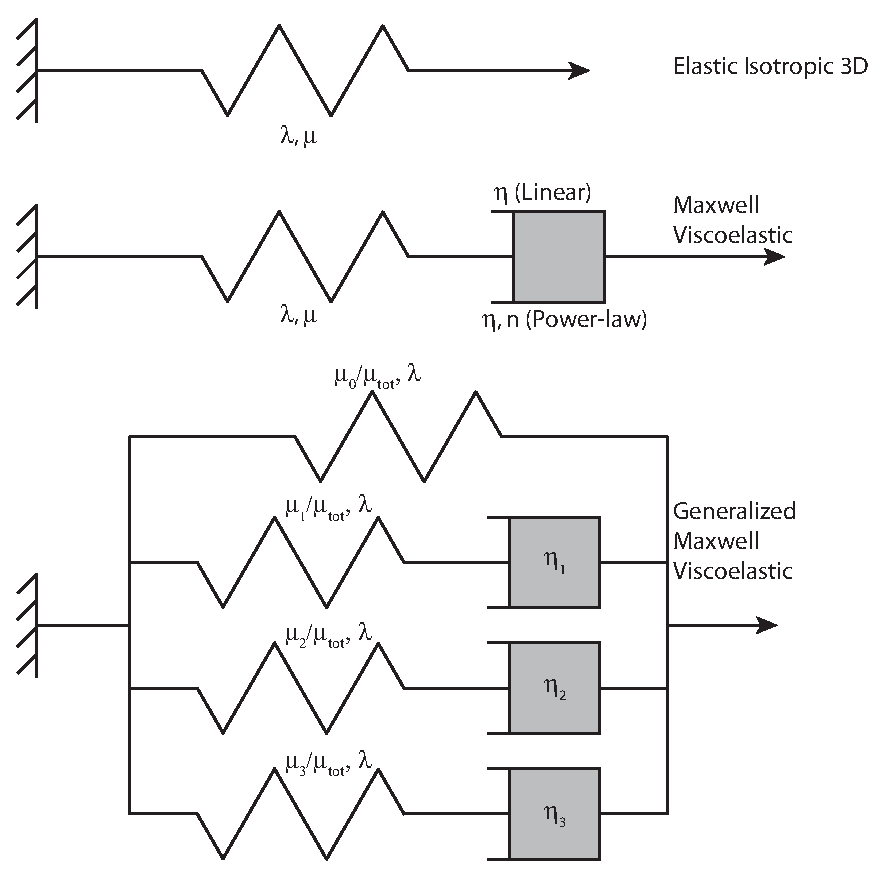
\includegraphics[scale=0.75]{materials/figs/pylith-materials}\caption{\label{fig:material:models}Spring-dashpot 1D representations of the
available 3D elastic and 2D/3D viscoelastic material models for PyLith.
The top model is a linear elastic model, the middle model is a Maxwell
model, and the bottom model is a generalized Maxwell model. For the
generalized Maxwell model, $\lambda$ and $\mu_{tot}$ are specified
for the entire model, and then the ratio $\mu_{i}/\mu_{tot}$ is specified
for each Maxwell model. For the power-law model, the linear dashpot
in the Maxwell model is replaced by a nonlinear dashpot obeying a
power-law.}
\end{figure}

\par\end{center}


\subsection{Definitions}

In the following sections, we use a combination of vector and index
notation (our notation conventions are shown in Table \vref{tab:notation}).
When using index notation, we use the common convention where repeated
indices indicate summation over the range of the index. We also make
frequent use of the scalar inner product. The scalar inner product
of two second-order tensors may be written
\begin{gather}
\underline{a}\cdot\underline{b}=a_{ij}b_{ij}\,.\label{eq:14}
\end{gather}
Although the general constitutive relations are formulated in terms
of the stress and strain, we frequently make use of the deviatoric
stress and strain in our formulation. We first define the mean stress,
$P$, and mean strain, $\theta$:
\begin{gather}
P=\frac{\sigma_{ii}}{3}\,,\,\,\,\,\theta=\frac{\epsilon_{ii}}{3}\,,\label{eq:15}
\end{gather}
where the $\sigma_{ii}$ and $\epsilon_{ii}$ represent the trace
of the stress and strain tensors, respectively. We then define the
deviatoric components of stress and strain as
\begin{gather}
S_{ij}=\sigma_{ij}-P\delta_{ij}\,,\,\,\,\, e_{ij}=\epsilon_{ij}-\theta\delta_{ij}\,,\label{eq:16}
\end{gather}
where $\delta_{ij}$ is the Kronecker delta. Using the deviatoric
components, we define the effective stress, $\overline{\sigma}$,
the second deviatoric stress invariant, $J_{2}^{\prime}$, the effective
deviatoric strain, $\overline{e}$, and the second deviatoric strain
invariant, $L_{2}^{\prime}$, as
\begin{gather}
\overline{\sigma}=\sqrt{\frac{3}{2}\underline{S}\cdot\underline{S}}\,\,\nonumber \\
J_{2}^{\prime}=\frac{1}{2}\underline{S}\cdot\underline{S}\,.\label{eq:17}\\
\overline{e}=\sqrt{\frac{2}{3}\underline{e}\cdot\underline{e}}\,\,\nonumber \\
L_{2}^{\prime}=\frac{1}{2}\underline{e}\cdot\underline{e}\,\,\nonumber 
\end{gather}
Due to the symmetry of the stress and strain tensors, it is sometimes
convenient to represent them as vectors:
\begin{gather}
\overrightarrow{\sigma^{T}}=\left[\begin{array}{cccccc}
\sigma_{11} & \sigma_{22} & \sigma_{33} & \sigma_{12} & \sigma_{23} & \sigma_{31}\end{array}\right]\label{eq:18}\\
\overrightarrow{\epsilon^{T}}=\left[\begin{array}{cccccc}
\epsilon_{11} & \epsilon_{22} & \epsilon_{33} & \epsilon_{12} & \epsilon_{23} & \epsilon_{31}\end{array}\right]\:.\nonumber 
\end{gather}
Note that when taking the scalar inner product of two tensors represented
as vectors, it is necessary to double the products representing off-diagonal
terms.

For quantities evaluated over a specific time period, we represent
the initial time as a pvrefixed subscript and the end time as a pvrefixed
superscript. In cases where the initial time does not appear, it is
understood to be $-\infty$.

\noindent \begin{center}
\begin{table}[H]
\noindent \centering{}\caption{\label{tab:notation}Mathematical notation used in this
section.}
\begin{tabular}{|c|c|c|}
\hline 
Index notation & Vector notation & Description\tabularnewline
\hline 
\hline 
$a_{i}$ & $\overrightarrow{a}$ & Vector field a\tabularnewline
\hline 
$a_{ij}$ & $\underline{a}$ & Second order tensor field a\tabularnewline
\hline 
\end{tabular}
\end{table}

\par\end{center}


\subsection{Linear Viscoelastic Models}

Linear viscoelastic models are obtained by various combinations of
a linear elastic spring and a linear viscous dashpot in series or
parallel. The simplest example is probably the linear Maxwell model,
which consists of a spring in series with a dashpot, as shown in Figure
\vref{fig:material:models}. For a one-dimensional model, the response
is given by
\begin{equation}
\frac{d\epsilon_{Total}}{dt}=\frac{d\epsilon_{D}}{dt}+\frac{d\epsilon_{S}}{dt}=\frac{\sigma}{\eta}+\frac{1}{E}\frac{d\sigma}{dt}\:,
\end{equation}
where $\epsilon_{Total}$ is the total strain, $\epsilon_{D}$ is
the strain in the dashpot, $\epsilon_{S}$ is the strain in the spring,
$\sigma$ is the stress, $\eta$ is the viscosity of the dashpot,
and $E$ is the spring constant. When a Maxwell material is subjected
to constant strain, the stresses relax exponentially with time. When
a Maxwell material is subjected to a constant stress, there is an
immediate elastic strain, corresponding to the response of the spring,
and a viscous strain that increases linearly with time. Since the
strain response is unbounded, the Maxwell model actually represents
a fluid.

Another simple model is the Kelvin-Voigt model, which consists of
a spring in parallel with a dashpot. In this case, the one-dimensional
response is given by
\begin{equation}
\sigma\left(t\right)=E\epsilon\left(t\right)+\eta\frac{d\epsilon\left(t\right)}{dt}\:.
\end{equation}
As opposed to the Maxwell model, which represents a fluid, the Kelvin-Voigt
model represents a solid undergoing reversible, viscoelastic strain.
If the material is subjected to a constant stress, it deforms at a
decreasing rate, gradually approaching the strain that would occur
for a purely elastic material. When the stress is released, the material
gradually relaxes back to its undeformed state.

The most general form of linear viscoelastic model is the generalized
Maxwell model, which consists of a spring in parallel with a number
of Maxwell models (see Figure \vref{fig:material:models}). Using this
model, it is possible to represent a number of simpler viscoelastic
models. For example, a simple Maxwell model is obtained by setting
the elastic constants of all springs to zero, with the exception of
the spring contained in the first Maxwell model ($\mu_{1}$). Similarly,
the Kelvin-Voigt model may be obtained by setting the elastic constants
$\mu_{2}=\mu_{3}=0$, and setting $\mu_{1}=\infty$ (or a very large
number).


\subsection{Formulation for Generalized Maxwell Models\label{sub:Formulation-for-Gen-Max}}

As described above, the generalized Maxwell viscoelastic model consists
of a number of Maxwell linear viscoelastic models in parallel with
a spring, as shown in Figure \vref{fig:material:models}. PyLith includes
the specific case of a spring in parallel with three Maxwell models.
As described in the previous paragraph, a number of common material
models may be obtained from this model by setting the shear moduli
of various springs to zero or infinity (or a large number), such as
the Maxwell model, the Kelvin model, and the standard linear solid.
We follow formulations similar to those used by Zienkiewicz and Taylor
\cite{Zienkiewicz:Taylor:2000} and Taylor \cite{Taylor:2003}. In
this formulation, we specify the total shear modulus of the model
($\mu_{tot}$) and Lame's constant ($\lambda$). We then provide the
fractional shear modulus for each Maxwell element spring in the model.
It is not necessary to specify the fractional modulus for $\mu_{0}$,
since this is obtained by subtracting the sum of the other ratios
from 1. Note that the sum of all these fractions must equal 1. We
use a similar formulation for our linear Maxwell viscoelastic model,
but in that case $\mu_{0}$ is always zero and we only use a single
Maxwell model. The parameters defining the standard Maxwell model
are shown in Table \vref{tab:linearMaxwell}, and those defining the
generalized Maxwell model are shown in Table \vref{tab:genMaxwell}.

As for all our viscoelastic models, the volumetric strain is completely
elastic, and the viscoelastic deformation may be expressed purely
in terms of the deviatoric components:
\begin{equation}
\underline{S}=2\mu_{tot}\left[\mu_{0}\underline{e}+\sum_{i=1}^{N}\mu_{i}\underline{q}^{i}-\underline{e}^{I}\right]+\underline{S}^{I}\,;\; P=3K\left(\theta-\theta^{I}\right)+P^{I}\,,\label{eq:19}
\end{equation}
where \textsl{K} is the bulk modulus, $N$ is the number of Maxwell
models, and the variable $\underline{q}^{i}$ follows the evolution
equations
\begin{equation}
\underline{\dot{q}}^{i}+\frac{1}{\tau_{i}}\underline{q}^{i}=\underline{\dot{e}}.\label{eq:20}
\end{equation}
The $\tau_{i}$ are the relaxation times for each Maxwell model:
\begin{equation}
\tau_{i}=\frac{\eta_{i}}{\mu_{tot}\mu_{i}}\:.\label{eq:21-1}
\end{equation}


An alternative to the differential equation form above is an integral
equation form expressed in terms of the relaxation modulus function.
This function is defined in terms of an idealized experiment in which,
at time labeled zero ($t=0$), a specimen is subjected to a constant
strain, $\underline{e}_{0}$, and the stress response, $\underline{S}\left(t\right)$,
is measured. For a linear material we obtain:
\begin{equation}
\underline{S}\left(t\right)=2\mu\left(t\right)\left(\underline{e}_{0}-\underline{e}^{I}\right)+\underline{S}^{I}\,,\label{eq:21}
\end{equation}
where $\mu\left(t\right)$ is the shear relaxation modulus function.
Using linearity and superposition for an arbitrary state of strain
yields an integral equation:
\begin{equation}
\underline{S}\left(t\right)=\intop_{-\infty}^{t}\mu\left(t-T\right)\underline{\dot{e}}\, dT\,.\label{eq:22}
\end{equation}
If we assume the modulus function in Prony series form we obtain
\begin{equation}
\mu\left(t\right)=\mu_{tot}\left(\mu_{0}+\sum_{i=1}^{N}\mu_{i}\exp\frac{-t}{\tau_{i}}\right)\,,\label{eq:23}
\end{equation}
where
\begin{equation}
\mu_{0}+\sum_{i=1}^{N}\mu_{i}=1\,.\label{eq:24}
\end{equation}
With the form in Equation \vref{eq:23}, the integral equation form
is identical to the differential equation form.

If we assume the material is undisturbed until a strain is suddenly
applied at time zero, we can divide the integral into
\begin{equation}
\intop_{-\infty}^{t}\left(\cdot\right)\, dT=\intop_{-\infty}^{0^{-}}\left(\cdot\right)\, dT+\intop_{0^{-}}^{0^{+}}\left(\cdot\right)\, dT+\intop_{0^{+}}^{t}\left(\cdot\right)\, dT\,.\label{eq:27}
\end{equation}
The first term is zero, the second term includes a jump term associated
with $\underline{e}_{0}$ at time zero, and the last term covers the
subsequent history of strain. Applying this separation to Equation
\vref{eq:22},
\begin{equation}
\underline{S}\left(t\right)=2\mu\left(t\right)\left(\underline{e}_{0}-\underline{e}^{I}\right)+\underline{S}^{I}+2\int_{0}^{t}\mu\left(t-T\right)\underline{\dot{e}}\left(T\right)\, dT\,,\label{eq:28}
\end{equation}
where we have left the sign off of the lower limit on the integral.

Substituting Equation \vref{eq:23} into \vref{eq:28}, we obtain
\begin{equation}
\underline{S}\left(t\right)=2\mu_{tot}\left\{ \mu_{0}\underline{e}\left(t\right)+\sum_{i=1}^{N}\left[\mu_{i}\exp\frac{-t}{\tau_{i}}\left(\underline{e}_{0}+\intop_{0}^{t}\exp\frac{t}{\tau_{i}}\underline{\dot{e}}\left(T\right)\, dT\right)\right]-\underline{e}^{I}\right\} +\underline{S}^{I}\,.\label{eq:29}
\end{equation}
We then split each integral into two ranges: from 0 to $t_{n}$, and
from $t_{n}$ to $t$, and define each integral as
\begin{equation}
\underline{i}_{i}^{1}\left(t\right)=\intop_{0}^{t}\exp\frac{T}{\tau_{i}}\underline{\dot{e}}\left(T\right)\, dT\,.\label{eq:30}
\end{equation}
The integral then becomes
\begin{equation}
\underline{i}_{i}^{1}\left(t\right)=\underline{i}_{i}^{1}\left(t_{n}\right)+\intop_{t_{n}}^{t}\exp\frac{T}{\tau_{i}}\underline{\dot{e}}\left(T\right)\, dT\,.\label{eq:31}
\end{equation}
Including the negative exponential multiplier:
\begin{equation}
\underline{h}_{i}^{1}\left(t\right)=\exp\frac{-t}{\tau_{i}}\underline{i}_{i}^{1}\,.\label{eq:32}
\end{equation}
Then
\begin{equation}
\underline{h}_{i}^{1}\left(t\right)=\exp\frac{-\Delta t}{\tau_{i}}\underline{h}_{i}^{1}\left(t_{n}\right)+\Delta\underline{h}_{i}\,,\label{eq:33}
\end{equation}
where
\begin{equation}
\Delta\underline{h}_{i}=\exp\frac{-t}{\tau_{i}}\intop_{t_{n}}^{t}\exp\frac{T}{\tau_{i}}\underline{\dot{e}}\left(T\right)\, dT\,.\label{eq:34}
\end{equation}
Approximating the strain rate as constant over each time step, the
solution may be found as
\begin{equation}
\Delta\underline{h}_{i}=\frac{\tau_{i}}{\Delta t}\left(1-\exp\frac{-\Delta t}{\tau_{i}}\right)\left(\underline{e}-\underline{e}_{n}\right)=\Delta h_{i}\left(\underline{e}-\underline{e}_{n}\right)\,.\label{eq:35}
\end{equation}
The approximation is singular for zero time steps, but a series expansion
may be used for small time-step sizes:
\begin{equation}
\Delta h_{i}\approx1-\frac{1}{2}\left(\frac{\Delta t}{\tau_{i}}\right)+\frac{1}{3!}\left(\frac{\Delta t}{\tau_{i}}\right)^{2}-\frac{1}{4!}\left(\frac{\Delta t}{\tau_{i}}\right)^{3}+\cdots\,.\label{eq:36}
\end{equation}
This converges with only a few terms. With this formulation, the constitutive
relation now has the simple form:
\begin{equation}
\underline{S}\left(t\right)=2\mu_{tot}\left(\mu_{0}\underline{e}\left(t\right)+\sum_{i=1}^{N}\mu_{i}\underline{h}_{i}^{1}\left(t\right)-\underline{e}^{I}\right)+\underline{S}^{I}\,.\label{eq:37}
\end{equation}


We need to compute the tangent constitutive matrix when forming the
stiffness matrix. In addition to the volumetric contribution to the
tangent constitutive matrix, we require the deviatoric part:
\begin{equation}
\frac{\partial\underline{S}}{\partial\underline{\epsilon}}=\frac{\partial\underline{S}}{\partial\underline{e}}\frac{\partial\underline{e}}{\partial\underline{\epsilon}}\,,\label{eq:38}
\end{equation}
where the second derivative on the right may be easily deduced from
Equation \vref{eq:16}. The other derivative is given by
\begin{equation}
\frac{\partial\underline{S}}{\partial\underline{e}}=2\mu_{tot}\left[\mu_{0}\underline{I}+\sum_{i=1}^{N}\mu_{i}\frac{\partial\underline{h}_{i}^{1}}{\partial\underline{e}}\right]\,,\label{eq:39}
\end{equation}
where $\underline{I}$ is the identity matrix. From Equations \vref{eq:33}
through \vref{eq:35}, the derivative inside the brackets is
\begin{equation}
\frac{\partial\underline{h}_{i}^{1}}{\partial\underline{e}}=\Delta h_{i}\left(\Delta t\right)\underline{I}\,.\label{eq:40}
\end{equation}
The complete deviatoric tangent relation is then
\begin{equation}
\frac{\partial\underline{S}}{\partial\underline{\epsilon}}=2\mu_{tot}\left[\mu_{0}+\sum_{i=1}^{N}\mu_{i}\Delta h_{i}\left(\Delta t\right)\right]\frac{\partial\underline{e}}{\partial\underline{\epsilon}}\,.\label{eq:41}
\end{equation}


We use this formulation for both our Maxwell and generalized Maxwell
viscoelastic models. For the Maxwell model, $\mu_{0}=0$ and $N=1$.
For the generalized Maxwell model, $N=3.$ The stable time step is
equal to 1/5 of the minimum relaxation time for all of the Maxwell
models (equation \vref{eq:21-1}).

\noindent \begin{center}
\begin{table}[H]
\noindent \centering{}\caption{\label{tab:linearMaxwell}Values in spatial databases for the linear
Maxwell viscoelastic material constitutive model.}
\begin{tabular}{|l|l|l|}
\hline 
\textbf{Spatial database} & \textbf{Value} & \textbf{Description}\tabularnewline
\hline 
\hline 
\multirow{4}{*}{\texttt{db\_properties}} & \texttt{vp} & Compressional wave speed, $v_{p}$\tabularnewline
\cline{2-3} 
 & \texttt{vs} & Shear wave speed, $v_{s}$\tabularnewline
\cline{2-3} 
 & \texttt{density} & Density, $\rho$\tabularnewline
\cline{2-3} 
 & \texttt{viscosity} & Viscosity, $\eta$\tabularnewline
\hline 
\texttt{db\_initial\_stress} & \texttt{stress-xx, }etc. & Initial stress components\tabularnewline
\hline 
\texttt{db\_initial\_strain} & \texttt{total-strain-xx, }etc. & Initial strain components\tabularnewline
\hline 
\multirow{2}{*}{\texttt{db\_initial\_state}} & \texttt{viscous-strain-xx, }etc. & Initial viscous strain components\tabularnewline
\cline{2-3} 
 & \texttt{stress-zz-initial} & Initial out-of-plane stress (2D only)\tabularnewline
\hline 
\end{tabular}
\end{table}

\par\end{center}

\noindent \begin{center}
\begin{table}[H]
\noindent \centering{}\caption{\label{tab:genMaxwell}Values in spatial database used as parameters
in the generalized linear Maxwell viscoelastic material constitutive
model.}
\begin{tabular}{|l|l|l|}
\hline 
\textbf{Spatial database} & \textbf{Value} & \textbf{Description}\tabularnewline
\hline 
\hline 
\multirow{9}{*}{\texttt{db\_properties}} & \texttt{vp} & Compressional wave speed, $v_{p}$\tabularnewline
\cline{2-3} 
 & \texttt{vs} & Shear wave speed, $v_{s}$\tabularnewline
\cline{2-3} 
 & \texttt{density} & Density, $\rho$\tabularnewline
\cline{2-3} 
 & \texttt{shear-ratio-1} & Shear ratio for Maxwell model 1, $\mu_{1}/\mu_{tot}$\tabularnewline
\cline{2-3} 
 & \texttt{shear-ratio-2} & Shear ratio for Maxwell model 2, $\mu_{2}/\mu_{tot}$\tabularnewline
\cline{2-3} 
 & \texttt{shear-ratio-3} & Shear ratio for Maxwell model 3, $\mu_{3}/\mu_{tot}$\tabularnewline
\cline{2-3} 
 & \texttt{viscosity-1} & Viscosity for Maxwell model 1, $\eta_{1}$\tabularnewline
\cline{2-3} 
 & \texttt{viscosity-2} & Viscosity for Maxwell model 2, $\eta_{2}$\tabularnewline
\cline{2-3} 
 & \texttt{viscosity-3} & Viscosity for Maxwell model 3, $\eta_{3}$\tabularnewline
\hline 
\texttt{db\_initial\_stress} & \texttt{stress-xx, }etc. & Initial stress components\tabularnewline
\hline 
\texttt{db\_initial\_strain} & \texttt{total-strain-xx, }etc. & Initial strain components\tabularnewline
\hline 
\multirow{4}{*}{\texttt{db\_initial\_state}} & \texttt{viscous-strain-1-xx, }etc. & Initial viscous strain components for Maxwell model 1\tabularnewline
\cline{2-3} 
 & \texttt{viscous-strain-2-xx, }etc. & Initial viscous strain components for Maxwell model 2\tabularnewline
\cline{2-3} 
 & \texttt{viscous-strain-3-xx, }etc. & Initial viscous strain components for Maxwell model 3\tabularnewline
\cline{2-3} 
 & \texttt{stress-zz-initial} & Initial out-of-plane stress (2D only)\tabularnewline
\hline 
\end{tabular}
\end{table}

\par\end{center}


\subsection{\label{sub:Effective-Stress-Formulations-Viscoelastic}Effective
Stress Formulations for Viscoelastic Materials}

As an alternative to the approach outlined above, an effective stress
function formulation \cite{Kojic:Bathe:1987} may be employed for
both a linear Maxwell model and a power-law Maxwell model. Note that
this formulation is not presently employed for linear viscoelastic
models (see Appendix \vref{cha:materials:alternative:formulations}), but it
is used for power-law viscoelastic materials. For the viscoelastic
materials considered here, the viscous volumetric strains are zero
(incompressible flow), and it is convenient to separate the general
stress-strain relationship at time $t+\Delta t$ into deviatoric and
volumetric parts:
\begin{gather}
\phantom{}{}^{t+\Delta t}\underline{S}=\frac{E}{1+\nu}\left(^{t+\Delta t}\underline{e}-\phantom{}^{t+\Delta t}\underline{e}^{C}-\underline{e}^{I}\right)+\underline{S}^{I}=\frac{1}{a_{E}}\left(^{t+\Delta t}\underline{e}-\phantom{}^{t+\Delta t}\underline{e}^{C}-\underline{e}^{I}\right)\label{eq:42}\\
^{t+\Delta t}P=\frac{E}{1-2\nu}\left(^{t+\Delta t}\theta-\theta^{I}\right)+P^{I}=\frac{1}{a_{m}}\left(^{t+\Delta t}\theta-\theta^{I}\right)\:,\nonumber 
\end{gather}
where $^{t+\Delta t}\underline{e}$ is the total deviatoric strain,
$^{t+\Delta t}\underline{e}^{C}$ is the total viscous strain, $\underline{e}^{I}$
is the initial deviatoric strain, $^{t+\Delta t}P$ is the pressure,
$^{t+\Delta t}\theta$ is the mean strain evaluated at time $t+\Delta t$
, and $\theta^{I}$ is the initial mean strain. The initial deviatoric
stress and initial pressure are given by $\underline{S}^{I}$ and
$P^{I}$, respectively. The topmost equation in Equation \vref{eq:42}
may also be written as
\begin{gather}
^{t+\Delta t}\underline{S}=\frac{1}{a_{E}}(^{t+\Delta t}\underline{e}^{\prime}-\underline{\Delta e}^{C})+\underline{S}^{I}\,,\label{eq:43}
\end{gather}
where
\begin{gather}
^{t+\Delta t}\underline{e}^{\prime}=\phantom{}^{t+\Delta t}\underline{e}-\phantom{}^{t}\underline{e}^{C}-\underline{e}^{I}\,\,,\,\,\,\underline{\Delta e}^{C}=\phantom{}^{t+\Delta t}\underline{e}^{C}-\phantom{}^{t}\underline{e}^{C}\,.\label{eq:44}
\end{gather}
The creep strain increment is approximated using
\begin{gather}
\underline{\Delta e}^{C}=\Delta t\phantom{}^{\tau}\gamma\phantom{}^{\tau}\underline{S}\,,\label{eq:45}
\end{gather}
where, using the $\alpha$-method of time integration,
\begin{gather}
^{\tau}\underline{S}=(1-\alpha)_{I}^{t}\underline{S}+\alpha\phantom{}_{I}^{t+\Delta t}\underline{S}+\underline{S}^{I}=(1-\alpha)^{t}\underline{S}+\alpha\phantom{}^{t+\Delta t}\underline{S}\,\,,\label{eq:46}
\end{gather}
and
\begin{gather}
^{\tau}\gamma=\frac{3\Delta\overline{e}^{C}}{2\Delta t\phantom{}^{\tau}\overline{\sigma}}\,\,,\label{eq:47}
\end{gather}
where
\begin{gather}
\Delta\overline{e}^{C}=\sqrt{\frac{2}{3}\underline{\Delta e}^{C}\cdot\underline{\Delta e}^{C}}\label{eq:48}
\end{gather}
and
\begin{gather}
^{\tau}\overline{\sigma}=(1-\alpha)_{I}^{t}\overline{\sigma}+\alpha\phantom{}_{I}^{t+\Delta t}\overline{\sigma}+\overline{\sigma}^{I}=\sqrt{3\phantom{}^{\tau}J_{2}^{\prime}}\,\,.\label{eq:49}
\end{gather}


To form the global stiffness matrix, it is necessary to provide a
relationship for the viscoelastic tangent material matrix relating
stress and strain. If we use vectors composed of the stresses and
tensor strains, this relationship is
\begin{gather}
\underline{C}^{VE}=\frac{\partial\phantom{}^{t+\Delta t}\overrightarrow{\sigma}}{\partial\phantom{}^{t+\Delta t}\overrightarrow{\epsilon}}\,\,.\label{eq:55}
\end{gather}
In terms of the vectors, we have
\begin{gather}
^{t+\Delta t}\sigma_{i}=\phantom{}^{t+\Delta t}S_{i}+\phantom{}^{t+\Delta t}P\,\,;\,\,\, i=1,2,3\label{eq:56}\\
^{t+\Delta t}\sigma_{i}=\phantom{}^{t+\Delta t}S_{i}\,;\,\,\,\,\,\,\,\,\,\,\,\,\,\,\,\,\,\,\,\,\,\,\,\,\,\,\,\,\,\,\, i=4,5,6\nonumber 
\end{gather}
Thevrefore,
\begin{gather}
C_{ij}^{VE}=C_{ij}^{\prime}+\frac{1}{3a_{m}}\,;\,\,1\leq i,j\leq3\,\,.\label{eq:57}\\
C_{ij}^{VE}=C_{ij}^{\prime}\,;\,\,\,\,\,\,\,\,\,\,\,\,\,\,\,\,\,\,\,\,\,\,\,\,\,\,\,\,\,\,\,\,\,\,\,\textrm{otherwise}\nonumber 
\end{gather}
Using the chain rule,
\begin{gather}
C_{ij}^{\prime}=\frac{\partial\phantom{}^{t+\Delta t}S_{i}}{\partial\phantom{}^{t+\Delta t}\epsilon_{j}}=\frac{\partial\phantom{}^{t+\Delta t}S_{i}}{\partial\phantom{}^{t+\Delta t}e_{k}^{\prime}}\frac{\partial\phantom{}^{t+\Delta t}e_{k}^{\prime}}{\partial\phantom{}^{t+\Delta t}e_{l}}\frac{\partial\phantom{}^{t+\Delta t}e_{l}}{\partial\phantom{}^{t+\Delta t}\epsilon_{j}}\,\,.\label{eq:58}
\end{gather}
From Equation \vref{eq:44}, we obtain
\begin{gather}
\frac{\partial\phantom{}^{t+\Delta t}e_{k}^{\prime}}{\partial\phantom{}^{t+\Delta t}e_{l}}=\delta_{kl}\,\,,\label{eq:59}
\end{gather}
and from Equation \vref{eq:16}:
\begin{gather}
\frac{\partial\phantom{}^{t+\Delta t}e_{l}}{\partial\phantom{}^{t+\Delta t}\epsilon_{j}}=\frac{1}{3}\left[\begin{array}{ccc}
2 & -1 & -1\\
-1 & 2 & -1\\
-1 & -1 & 2
\end{array}\right];\,\,1\leq l,j\leq3\label{eq:60}\\
\frac{\partial\phantom{}^{t+\Delta t}e_{l}}{\partial\phantom{}^{t+\Delta t}\epsilon_{j}}=\delta_{lj}\,\,;\,\,\,\,\,\,\,\,\,\,\,\,\,\,\,\,\,\,\,\,\,\,\,\,\,\,\,\,\,\,\,\,\,\,\,\,\,\,\,\,\,\,\,\,\textrm{otherwise.}\nonumber 
\end{gather}
The first term of Equation \vref{eq:58} depends on the particular
constitutive relationship, and the complete tangent matrix may then
be obtained from Equation \vref{eq:57}.


\subsubsection{Power-Law Maxwell Viscoelastic Material\label{sub:Power-Law-Maxwell-Viscoelastic}}

Laboratory results on rock rheology are typically performed using
a triaxial experiment, and the creep data are fit to a power-law equation
of the form (e.g., \cite{Kirby:Kronenberg:1987}):
\begin{equation}
\dot{\epsilon}_{11}^{C}=A_{E}\exp\left(\frac{-Q}{RT}\right)\left(\sigma_{1}-\sigma_{3}\right)^{n}=A_{E}\exp\left(\frac{-Q}{RT}\right)\sigma_{d}^{n}\:,\label{eq:64}
\end{equation}
where $\dot{\epsilon}_{11}^{C}$ is the strain rate in the direction
of the maximum principal stress $\left(\sigma_{1}\right)$, $A_{E}$
is the experimentally-derived pre-exponential constant, $Q$ is the
activation enthalpy, $R$ is the universal gas constant, $T$ is the
absolute temperature, $n$ is the power-law exponent, $\sigma_{3}\:\left(=\sigma_{2}\right)$
is equal to the confining pressure, and $\sigma_{d}$ is the differential
stress. To properly formulate the flow law, it must be generalized
so that the results are not influenced by the experiment type or the
choice of coordinate systems (e.g., \cite{Paterson:1994}). The flow
law may then be generalized in terms of the deviatoric stress and
strain rate invariants:
\begin{equation}
\sqrt{\dot{L}_{2}^{\prime C}}=A_{M}\exp\left(\frac{-Q}{RT}\right)\sqrt{J_{2}^{\prime}}^{n}\:,\label{eq:65}
\end{equation}
where $A_{M}$ is now a pre-exponential constant used in the formulation
for modeling. In practice, it is necessary to compute each strain
rate component using the flow law. This is accomplished using:
\begin{equation}
\dot{e}_{ij}^{C}=A_{M}\exp\left(\frac{-Q}{RT}\right)\sqrt{J_{2}^{\prime}}^{n-1}S_{ij}\:.\label{eq:66}
\end{equation}
Note that Equations \vref{eq:65} and \vref{eq:66} are consistent,
since Equation \vref{eq:65} may be obtained from Equation \vref{eq:66}
by taking the scalar inner product of both sides, multiplying by 1/2,
and taking the square root.

In a triaxial experiment with confining pressure $P_{c}$, we have
\begin{gather}
\sigma_{2}=\sigma_{3}=P_{c}\nonumber \\
\sigma_{1}=\sigma_{1}^{app}\label{eq:67}\\
P=\frac{\sigma_{1}+2P_{c}}{3}\:,\nonumber 
\end{gather}
where $\sigma_{1}^{app}$ is the applied load. The deviatoric stresses
are then:
\begin{gather}
S_{1}=\frac{2}{3}\left(\sigma_{1}-P_{c}\right)\nonumber \\
S_{2}=S_{3}=-\frac{1}{3}\left(\sigma_{1}-P_{c}\right)\:.\label{eq:68}
\end{gather}
This gives
\begin{gather}
S_{1}=\frac{2}{3}\left(\sigma_{1}-\sigma_{3}\right)=\frac{2}{3}\sigma_{d}\nonumber \\
S_{2}=S_{3}=-\frac{1}{3}\left(\sigma_{1}-\sigma_{3}\right)=-\frac{1}{3}\sigma_{d}\:.\label{eq:69}
\end{gather}
In terms of the second deviatoric stress invariant, we then have
\begin{equation}
\sqrt{J_{2}^{\prime}}=\frac{\sigma_{d}}{\sqrt{3}}\:.\label{eq:70}
\end{equation}


Under the assumption that the creep measured in the laboratory experiments
is incompressible, we have
\begin{gather}
\dot{e}_{11}^{C}=\dot{\epsilon}_{11}\nonumber \\
\dot{e}_{22}^{C}=\dot{e}_{33}^{C}=-\frac{1}{2}\dot{\epsilon}_{11}\:.\label{eq:71}
\end{gather}
In terms of the second deviatoric strain rate invariant we then have
\begin{equation}
\sqrt{\dot{L}_{2}^{\prime C}}=\frac{\sqrt{3}}{2}\dot{\epsilon}_{11}\:.\label{eq:72}
\end{equation}
Substituting Equations \vref{eq:70} and \vref{eq:72} into Equation
\vref{eq:64}, we obtain
\begin{equation}
\sqrt{\dot{L}_{2}^{\prime C}}=A_{E}\frac{\sqrt{3}^{n+1}}{2}\exp\left(\frac{-Q}{RT}\right)\sqrt{J_{2}^{\prime}}^{n}\:,\label{eq:73}
\end{equation}
and thevrefore,
\begin{equation}
A_{M}=\frac{\sqrt{3}^{n+1}}{2}A_{E}\:.\label{eq:74}
\end{equation}
When the exponential factor is included, we define a new parameter:

\begin{equation}
A_{T}=A_{M}\exp\left(\frac{-Q}{RT}\right)=\frac{\sqrt{3}^{n+1}}{2}A_{E}\exp\left(\frac{-Q}{RT}\right)\:.\label{eq:75}
\end{equation}


There is a problem with the usage of parameters $A_{E}$, $A_{M}$,
and $A_{T}$. Since the dimensions of these parameters are dependent
on the value of the power-law exponent, they are not really constants.
In addition to being logically inconsistent, this presents problems
when specifying parameters for PyLith, since the power-law exponent
must be known before the units can be determined. An alternative way
of writing the flow rule is (e.g., \cite{Prentice:1968}): 
\begin{equation}
\frac{\sqrt{\dot{L}_{2}^{\prime C}}}{\dot{e}_{0}}=\left(\frac{\sqrt{J_{2}^{\prime}}}{S_{0}}\right)^{n},\label{eq:76}
\end{equation}
where $\dot{e}_{0}$ and $S_{0}$ are vreference values for the strain
rate and deviatoric stress. This means that
\begin{equation}
\frac{\dot{e}_{0}}{S_{0}^{n}}=A_{T}\:.\label{eq:77}
\end{equation}
Users must thevrefore specify three parameters for a power-law material.
The properties \texttt{vreference-strain-rate}, \texttt{vreference-stress},
and \texttt{power-law-exponent} in Table \vref{tab:powerLaw} vrefer
to $\dot{e}_{0}$, $S_{0}$, and $n$, respectively. To specify the
power-law properties for PyLith using laboratory results, the user
must first compute $A_{T}$ using Equation \vref{eq:75}. Then, values
for $\dot{e}_{0}$ and $S_{0}$ must be provided. The simplest method
is probably to assume a reasonable value for the vreference strain
rate, and then compute $S_{0}$ as
\begin{equation}
S_{0}=\left(\frac{\dot{e}_{0}}{A_{T}}\right)^{\frac{1}{n}}\:.\label{eq:78}
\end{equation}


A utility code (\texttt{powerlaw\_gendb.py}) is provided to convert
laboratory results to the properties used by PyLith. To use the code,
users must specify the spatial variation of $A_{E}$, $Q$, $n$,
and $T$. An additional parameter is given to define the units of
$A_{E}$. The user then specifies either a vreference stress or a vreference
strain rate, and a database suitable for PyLith is generated. This
utility is described more fully in Section \vref{sub:Tutorial-Step08-Power-law}.

The flow law in component form is 
\begin{equation}
\dot{e}_{ij}^{C}=\frac{\dot{e}_{0}\sqrt{J_{2}^{\prime}}^{n-1}S_{ij}}{S_{0}^{n}}\:,\label{eq:79}
\end{equation}
and the creep strain increment is approximated as
\begin{gather}
\underline{\Delta e}^{C}\approx\frac{\Delta t\dot{e}_{0}\sqrt{^{\tau}J_{2}^{\prime}}^{n-1}\,^{\tau}\underline{S}}{S_{0}^{n}}=\frac{\Delta t\dot{e}_{0}\phantom{}^{\tau}\overline{\sigma}^{n-1}\,^{\tau}\underline{S}}{\sqrt{3}S_{0}^{n}}\,.\label{eq:80}
\end{gather}
 Thevrefore,
\begin{gather}
\Delta\bar{e}^{C}\approx\frac{2\Delta t\dot{e}_{0}\sqrt{^{\tau}J_{2}^{\prime}}^{n}}{\sqrt{3}S_{0}^{n}}=\frac{2\Delta t\dot{e}_{0}\phantom{}^{\tau}\overline{\sigma}^{n}}{\sqrt{3}^{n+1}S_{0}^{n}}\,,\,\textrm{and}\,^{\tau}\gamma=\frac{\dot{e}_{0}\sqrt{^{\tau}J_{2}^{\prime}}^{n-1}}{S_{0}^{n}}\,.\label{eq:81}
\end{gather}
substituting Equations \vref{eq:46}, \vref{eq:80}, and \vref{eq:81}
into \vref{eq:43}, we obtain:
\begin{gather}
^{t+\Delta t}\underline{S}=\frac{1}{a_{E}}\left\{ ^{t+\Delta t}\underline{e}^{\prime}-\Delta t\phantom{}^{\tau}\gamma\left[\left(1-\alpha\right)^{t}\underline{S}+\alpha{}^{t+\Delta t}\underline{S}\right]\right\} +\underline{S}^{I}\,,\label{eq:82}
\end{gather}
which may be rewritten:
\begin{gather}
^{t+\Delta t}\underline{S}\left(a_{E}+\alpha\Delta t\phantom{}^{\tau}\gamma\right)={}^{t+\Delta t}\underline{e}^{\prime}-\Delta t\phantom{}^{\tau}\gamma\left(1-\alpha\right)^{t}\underline{S}+a_{E}\underline{S}^{I}\,.\label{eq:83}
\end{gather}
Taking the scalar inner product of both sides we obtain:
\begin{gather}
a^{2}\,\,{}^{t+\Delta t}J_{2}^{\prime}-b+c\phantom{}^{\tau}\gamma-d^{2}\,^{\tau}\gamma^{2}=F=0\,,\label{eq:84}
\end{gather}
where
\begin{gather}
a=a_{E}+\alpha\Delta t\phantom{}^{\tau}\gamma\,\,\nonumber \\
b=\frac{1}{2}{}^{t+\Delta t}\underline{e}^{\prime}\cdot{}^{t+\Delta t}\underline{e}^{\prime}+a_{E}{}^{t+\Delta t}\underline{e}^{\prime}\cdot\underline{S}^{I}+a_{E}^{2}\,^{I}J_{2}^{\prime}\,.\label{eq:85}\\
c=\Delta t\left(1-\alpha\right){}^{t+\Delta t}\underline{e}^{\prime}\cdot^{t}\underline{S}+\Delta t\left(1-\alpha\right)a_{E}\,^{t}\underline{S}\cdot\underline{S}^{I}\,\,\nonumber \\
d=\Delta t\left(1-\alpha\right)\sqrt{^{t}J_{2}^{\prime}}\,\,\nonumber 
\end{gather}
Equation \vref{eq:84} is a function of a single unknown -- the square
root of the second deviatoric stress invariant at time $t+\Delta t$
-- and may be solved by bisection or by Newton's method. Once this
parameter has been found, the deviatoric stresses for the current
time step may be found from Equations \vref{eq:49}, \vref{eq:81},
and \vref{eq:82}, and the total stresses may be found by combining
the deviatoric and volumetric components from Equation \vref{eq:42}.

Once the stresses are computed for the current time step, we can compute
the relaxation time (used in computing the stable time step) by first
computing the effective viscous strain rate from Equation \vref{eq:79}:
\begin{equation}
\dot{\bar{e}}^{C}=\frac{2\dot{e}_{0}\left(\frac{\bar{\sigma}}{\sqrt{3}}\right)^{n}}{\sqrt{3}S_{0}^{n}}\:.
\end{equation}
Similarly, the effective elastic strain is computed as:
\begin{equation}
\bar{e}^{E}=\frac{\bar{\sigma}}{3\mu}\:.
\end{equation}
The relaxation time is then the ratio between these two:
\begin{equation}
\tau=\frac{\bar{e}^{E}}{\bar{\dot{e}}^{C}}=\left(\frac{S_{0}}{\sqrt{J_{2}^{\prime}}}\right)^{n-1}\frac{S_{0}}{6\mu\dot{e}_{0}}\:.\label{eq:86-1}
\end{equation}
The stable time step returned by PyLith is 1/5 of the value computed
from Equation \vref{eq:86-1}.

To compute the tangent stress-strain relation, we need to compute
the first term in Equation \vref{eq:58}. We begin by rewriting Equation
\vref{eq:83} as
\begin{gather}
F=^{t+\Delta t}S_{i}\left(a_{E}+\alpha\Delta t\phantom{}^{\tau}\gamma\right)-\phantom{}^{t+\Delta t}e_{i}^{\prime}+\Delta t\phantom{}^{\tau}\gamma\left(1-\alpha\right)^{t}S_{i}-a_{E}S_{i}^{I}=0\:.\label{eq:86}
\end{gather}
The derivative of this function with respect to $^{t+\Delta t}e_{k}^{\prime\prime}$
is
\begin{gather}
\frac{\partial F}{\partial\phantom{}^{t+\Delta t}e_{k}^{\prime}}=-\delta_{ik}\:,\label{eq:87}
\end{gather}
and the derivative with respect to $^{t+\Delta t}S_{i}$ is
\begin{gather}
\frac{\partial F}{\partial\phantom{}^{t+\Delta t}S_{i}}=a_{E}+\alpha\Delta t\phantom{}^{\tau}\gamma+\frac{\partial\phantom{}^{\tau}\gamma}{\partial\phantom{}^{t+\Delta t}S_{i}}\Delta t\left[\alpha\phantom{}^{t+\Delta t}S_{i}+\left(1-\alpha\right)^{t}S_{i}\right]\:.\label{eq:88}
\end{gather}
From Equation \vref{eq:81} and Equation \vref{eq:49},
\begin{gather}
^{\tau}\gamma=\frac{\dot{e}_{0}}{S_{0}^{n}}\left[\alpha\sqrt{^{t+\Delta t}J_{2}^{\prime}}+\left(1-\alpha\right)\sqrt{^{t}J_{2}^{\prime}}\right]^{n-1}\:.\label{eq:89}
\end{gather}
Then
\begin{gather}
\frac{\partial\phantom{}^{\tau}\gamma}{\partial{}^{t+\Delta t}S_{i}}=\frac{\partial\phantom{}^{\tau}\gamma}{\partial\sqrt{^{t+\Delta t}J_{2}^{\prime}}}\frac{\partial\sqrt{^{t+\Delta t}J_{2}^{\prime}}}{\partial\phantom{}^{t+\Delta t}S_{l}}\label{eq:90}\\
=\frac{\dot{e}_{0}\alpha\left(n-1\right)\sqrt{^{\tau}J_{2}^{\prime}}^{n-2}{}^{t+\Delta t}T_{i}}{2S_{0}^{n}}\,,\nonumber 
\end{gather}
where
\begin{gather}
^{t+\Delta t}T_{i}=\phantom{}^{t+\Delta t}S_{i}\:;\:\:1\leq i\leq3\label{eq:91}\\
^{t+\Delta t}T_{i}=2\phantom{}^{t+\Delta t}S_{i}\:;\:\:\textrm{otherwise.}\nonumber 
\end{gather}
Then using Equations \vref{eq:87}, \vref{eq:88}, \vref{eq:90}, and
the quotient rule for derivatives of an implicit function,
\begin{gather}
\frac{\partial\phantom{}^{t+\Delta t}S_{i}}{\partial{}^{t+\Delta t}e_{k}^{\prime}}=\frac{\delta_{ik}}{a_{E}+\alpha\Delta t\left[^{\tau}\gamma+\frac{\dot{e}_{0}{}^{\tau}S_{i}\left(n-1\right){}^{t+\Delta t}T_{i}\sqrt{^{\tau}J_{2}^{\prime}}^{n-2}}{2\sqrt{^{t+\Delta t}J_{2}^{\prime}}S_{0}^{n}}\right]}\,.\label{eq:92}
\end{gather}
Note that for a linear material $\left(n=1\right)$, this equation
is identical to the linear formulation in Section \vref{sub:Effective-Stress-Formulation-Maxwell}
(making the appropriate substitution for $^{\tau}\gamma$). Then,
using Equations \vref{eq:57} through \vref{eq:60},
\begin{gather}
C_{ij}^{VE}=\frac{1}{3a_{m}}\left[\begin{array}{cccccc}
1 & 1 & 1 & 0 & 0 & 0\\
1 & 1 & 1 & 0 & 0 & 0\\
1 & 1 & 1 & 0 & 0 & 0\\
0 & 0 & 0 & 0 & 0 & 0\\
0 & 0 & 0 & 0 & 0 & 0\\
0 & 0 & 0 & 0 & 0 & 0
\end{array}\right]+\frac{1}{3}\frac{\partial{}^{t+\Delta t}S_{i}}{\partial{}^{t+\Delta t}e_{k}^{\prime}}\left[\begin{array}{cccccc}
2 & -1 & -1 & 0 & 0 & 0\\
-1 & 2 & -1 & 0 & 0 & 0\\
-1 & -1 & 2 & 0 & 0 & 0\\
0 & 0 & 0 & 3 & 0 & 0\\
0 & 0 & 0 & 0 & 3 & 0\\
0 & 0 & 0 & 0 & 0 & 3
\end{array}\right]\,.\label{eq:93}
\end{gather}
Note that if there are no deviatoric stresses at the beginning and
end of a time step (or if $\nicefrac{\dot{e}_{0}}{S_{0}^{n}}$ approaches
zero), Equations \vref{eq:92} and \vref{eq:93} reduce to the elastic
constitutive matrix, as expected.

To compute the zero of the effective stress function using Newton's
method, we require the derivative of Equation \vref{eq:84}, which
may be written:
\begin{gather}
\frac{\partial F}{\partial\sqrt{^{t+\Delta t}J_{2}^{\prime}}}=2a^{2}\sqrt{^{t+\Delta t}J_{2}^{\prime}}+\frac{\dot{e}_{0}\alpha\left(n-1\right)\sqrt{^{\tau}J_{2}^{\prime}}^{n-2}}{S_{0}^{n}}\left(2a\alpha\Delta t{}^{t+\Delta t}J_{2}^{\prime}+c-2d^{2}\,^{\tau}\gamma\right)\,.\label{eq:94}
\end{gather}


\noindent \begin{center}
\begin{table}[H]
\noindent \centering{}\caption{\label{tab:powerLaw}Values in spatial database used as parameters
in the nonlinear power-law viscoelastic material constitutive model.}
\begin{tabular}{|l|l|l|}
\hline 
\textbf{Spatial database} & \textbf{Value} & \textbf{Description}\tabularnewline
\hline 
\hline 
\multirow{6}{*}{\texttt{db\_properties}} & \texttt{vp} & Compressional wave speed, $v_{p}$\tabularnewline
\cline{2-3} 
 & \texttt{vs} & Shear wave speed, $v_{s}$\tabularnewline
\cline{2-3} 
 & \texttt{density} & Density, $\rho$\tabularnewline
\cline{2-3} 
 & \texttt{vreference-strain-rate} & Reference strain rate, $\dot{e}_{0}$\tabularnewline
\cline{2-3} 
 & \texttt{vreference-stress} & Reference stress, $S_{0}$\tabularnewline
\cline{2-3} 
 & \texttt{power-law-exponent} & Power-law exponent, $n$\tabularnewline
\hline 
\texttt{db\_initial\_stress} & \texttt{stress-xx, }etc. & Initial stress components\tabularnewline
\hline 
\texttt{db\_initial\_strain} & \texttt{total-strain-xx, }etc. & Initial strain components\tabularnewline
\hline 
\multirow{2}{*}{\texttt{db\_initial\_state}} & \texttt{viscous-strain-xx, }etc. & Initial viscous strain components\tabularnewline
\cline{2-3} 
 & \texttt{stress-zz-initial} & Initial out-of-plane stress (2D only)\tabularnewline
\hline 
\end{tabular}
\end{table}

\par\end{center}


\section{Elastoplastic Materials}

PyLith presently contains just a single elastoplastic material that
implements the Drucker-Prager yield criterion. Future releases of
PyLith may contain additional elastoplastic materials, such as Drucker-Prager
with hardening/softening.


\subsection{General Elastoplasticity Formulation}

The elastoplasticity formulation in PyLith is based on an additive
decomposition of the total strain into elastic and plastic parts:
\begin{equation}
d\epsilon_{ij}=d\epsilon_{ij}^{E}+d\epsilon_{ij}^{P}\:.\label{eq:95}
\end{equation}
The stress increment is then given by
\begin{equation}
d\sigma_{ij}=C_{ijrs}^{E}\left(d\epsilon_{rs}-d\epsilon_{rs}^{P}\right)\:,\label{eq:96}
\end{equation}
where $C_{ijrs}^{E}$ are the components of the elastic constitutive
tensor. To completely specify an elastoplastic problem, three components
are needed. We first require a yield condition, which specifies the
state of stress at which plastic flow initiates. This is generally
given in the form:
\begin{equation}
f\left(\underline{\sigma},k\right)=0\:,\label{eq:97}
\end{equation}
where \textit{k} is an internal state parameter. It is then necessary
to specify a flow rule, which describes the relationship between plastic
strain and stress. The flow rule is given in the form:
\begin{equation}
g\left(\underline{\sigma},k\right)=0\:.\label{eq:98}
\end{equation}
The plastic strain increment is then given as
\begin{equation}
d\epsilon_{ij}^{P}=d\lambda\frac{\partial g}{\partial\sigma_{ij}}\:,\label{eq:99}
\end{equation}
where $d\lambda$ is the scalar plastic multiplier. When the flow
rule is identical to the yield criterion ($f\equiv g$), the plasticity
is described as associated. Otherwise, it is non-associated. The final
component needed is a hardening hypothesis, which describes how the
yield condition and flow rule are modified during plastic flow. When
the yield condition and flow rule remain constant during plastic flow
(e.g., no hardening), the material is vreferred to as perfectly plastic.

To perform the solution, the yield condition (Equation \vref{eq:97})
is first evaluated under the assumption of elastic behavior. If $^{t+\Delta t}f<0$,
the material behavior is elastic and no plastic flow occurs. Otherwise,
the behavior is plastic and a plastic strain increment must be computed
to return the stress state to the yield envelope. This procedure is
known as an elastic predictor-plastic corrector algorithm.


\subsection{Drucker-Prager Elastoplastic Material}

PyLith includes an elastoplastic implementation of the Drucker-Prager
yield criterion \cite{Drucker:Prager:1952}. This criterion was originally
devised to model plastic deformation of soils, and it has also been
used to model rock deformation. It is intended to be a smooth approximation
of the Mohr-Coulomb yield criterion. The implementation used in PyLith
includes non-associated plastic flow, which allows control over the
unreasonable amounts of dilatation that are sometimes predicted by
the associated model. The model is described by the following yield
condition:
\begin{equation}
f\left(\underline{\sigma},k\right)=\alpha_{f}I_{1}+\sqrt{J_{2}^{\prime}}-\beta\:,\label{eq:100}
\end{equation}
and a flow rule given by:
\begin{equation}
g\left(\underline{\sigma},k\right)=\sqrt{J_{2}^{\prime}}+\alpha_{g}I_{1}\:.\label{eq:101}
\end{equation}


The yield surface represents a circular cone in principal stress space,
and the parameters can be related to the friction angle, $\phi$,
and the cohesion, $\bar{c}$, of the Mohr-Coulomb model. The yield
surface in Haigh-Westergaard space ($\zeta=\frac{1}{\sqrt{3}}I_{1},p=\sqrt{2J_{2}},\cos(3\theta)=\frac{3\sqrt{3}}{2}\frac{J_{3}}{J_{2}^{3/2}}$)
is
\begin{equation}
\left(\sqrt{3}\sin\left(\theta+\frac{\pi}{3}\right)-\sin\phi\cos\left(\theta+\frac{\pi}{3}\right)\right)p-\sqrt{2}\sin\phi\zeta=\sqrt{6}\overline{c}\cos\theta.\label{eq:drucker:prager:haigh:westergaard}
\end{equation}
The yield surface can be fit to the Mohr-Coulomb model in several
different ways. The yield surface can touch the outer apices ($\theta=\pi/3$)
of the Mohr-Coulomb model (inscribed version), the inner apices ($\theta=0$)
of the Mohr-Coulomb model (circumscribed version), or halfway between
the two ($\theta=pi/6,$middle version). Substituting these values
for $\theta$ into Equation (\vref{eq:drucker:prager:haigh:westergaard})
and casting it into the same form as Equation (\vref{eq:101}) yields
the values of $\alpha_{f}$, $\beta$, and $\alpha_{g}$ given in
Table \vref{tab:fit_mohr_coulomb}, where $\phi_{0}$ vrefers to the
initial friction angle. Similarly, the flow rule can be related to
the dilatation angle, $\psi$, of a Mohr-Coulomb model. It is also
possible for the Mohr-Coulomb parameters to be functions of the internal
state parameter, $k$. In PyLith, the fit to the Mohr-Coulomb yield
surface and flow rule is controlled by the \texttt{fit\_mohr\_coulomb}
property. 

\begin{table}
\caption{\label{tab:fit_mohr_coulomb}Options for fitting the Drucker-Prager
plastic parameters to a Mohr-Coulomb model using \texttt{fit\_mohr\_coulomb}.}


\centering{}%
\begin{tabular}{|c|c|c|c|}
\hline 
\textbf{Parameter Value} & $\alpha_{f}$ & $\beta$ & $\alpha_{g}$\tabularnewline
\hline 
\hline 
\texttt{inscribed} & $\frac{2\sin\phi\left(k\right)}{\sqrt{3}\left(3-\sin\phi\left(k\right)\right)}$ & $\frac{6\bar{c}\left(k\right)\cos\phi_{0}}{\sqrt{3}\left(3-\sin\phi_{0}\right)}$ & $\frac{2\sin\psi(k)}{\sqrt{3}\left(3-\sin\psi\left(k\right)\right)}$\tabularnewline
\hline 
\texttt{middle} & $\frac{\sin\phi\left(k\right)}{3}$ & $\bar{c}\left(k\right)\cos\left(\phi_{0}\right)$ & $\frac{\sin\psi\left(k\right)}{3}$\tabularnewline
\hline 
\texttt{circumscribed} & $\frac{2\sin\phi\left(k\right)}{\sqrt{3}\left(3+\sin\phi\left(k\right)\right)}$ & $\frac{6\bar{c}\left(k\right)\cos\phi_{0}}{\sqrt{3}\left(3+\sin\phi_{0}\right)}$ & $\frac{2\sin\psi(k)}{\sqrt{3}\left(3+\sin\psi\left(k\right)\right)}$\tabularnewline
\hline 
\end{tabular}
\end{table}


As for the viscoelastic models, it is convenient to separate the deformation
into deviatoric and volumetric parts:
\begin{gather}
^{t+\Delta t}S_{ij}=\frac{1}{a_{E}}\left(^{t+\Delta t}e_{ij}-\phantom{}^{t+\Delta t}e_{ij}^{P}-e_{ij}^{I}\right)+S_{ij}^{I}=\frac{1}{a_{E}}\left(^{t+\Delta t}e_{ij}^{\prime}-\Delta e_{ij}^{P}\right)+S_{ij}^{I}\label{eq:105}\\
^{t+\Delta t}P=\frac{1}{a_{m}}\left(^{t+\Delta t}\theta-\phantom{}^{t+\Delta t}\theta^{P}-\theta^{I}\right)+P^{I}=\frac{1}{a_{m}}\left(^{t+\Delta t}\theta^{\prime}-\Delta\theta^{P}\right)+P^{I}\:,\nonumber 
\end{gather}
where
\begin{gather}
^{t+\Delta t}e_{ij}^{\prime}=\phantom{}^{t+\Delta t}e_{ij}-\phantom{}^{t}e_{ij}^{P}-e_{ij}^{I}\nonumber \\
\Delta e_{ij}^{P}=\phantom{}^{t+\Delta t}e_{ij}^{P}-\phantom{}^{t}e_{ij}^{P}\nonumber \\
^{t+\Delta t}\theta^{\prime}=\phantom{}^{t+\Delta t}\theta-\phantom{}^{t}\theta^{P}-\theta^{I}\nonumber \\
\Delta\theta^{P}=\phantom{}^{t+\Delta t}\theta^{P}-\phantom{}^{t}\theta^{P}\:.\label{eq:106}
\end{gather}
Since the plasticity is pressure-dependent, there are volumetric plastic
strains, unlike the viscous strains in the previous section. From
Equation \vref{eq:99}, the plastic strain increment is
\begin{equation}
\Delta\epsilon_{ij}^{P}=\lambda\frac{\partial\phantom{}^{t+\Delta t}g}{\partial\phantom{}^{t+\Delta t}\sigma_{ij}}=\lambda\alpha_{g}\delta_{ij}+\lambda\frac{^{t+\Delta t}S_{ij}}{2\sqrt{^{t+\Delta t}J_{2}^{\prime}}}\:.\label{eq:107}
\end{equation}
The volumetric part is
\begin{equation}
\Delta\theta^{P}=\frac{1}{3}\Delta\epsilon_{ii}^{P}=\lambda\alpha_{g}\:,\label{eq:108}
\end{equation}
and the deviatoric part is
\begin{equation}
\Delta e_{ij}^{P}=\Delta\epsilon_{ij}^{P}-\Delta\epsilon_{m}^{P}\delta_{ij}=\lambda\frac{^{t+\Delta t}S_{ij}}{2\sqrt{^{t+\Delta t}J_{2}^{\prime}}}\:.\label{eq:109}
\end{equation}
The problem is reduced to solving for $\lambda$. The procedure is
different depending on whether hardening is included.


\subsubsection{Drucker-Prager Elastoplastic With No Hardening (Perfectly Plastic)}

When there is no hardening (perfect plasticity), the Drucker-Prager
elastoplastic model may be parameterized with just three parameters,
in addition to the normal elasticity parameters. The parameters \texttt{friction-angle},
\texttt{cohesion}, and \texttt{dilatation-angle} in Table \vref{tab:druckerPrager}
vrefer respectively to $\phi$, $\bar{c}$, and $\psi$ in Table \vref{tab:fit_mohr_coulomb}.
These are then converted to the properties $\alpha_{f}$ (\texttt{alpha-yield}),
$\beta$ (\texttt{beta}), and $\alpha_{g}$ (\texttt{alpha-flow}),
as shown in Table \vref{tab:material-model-output}.

For perfect plasticity the yield and flow functions do not vary, and
we can solve for $\lambda$ by substituting Equation \vref{eq:109}
into Equation \vref{eq:105} and taking the scalar inner product of
both sides:
\begin{equation}
\lambda=\sqrt{2}\,\phantom{}^{t+\Delta t}d-2a_{E}\sqrt{^{t+\Delta t}J_{2}^{\prime}}\:,\label{eq:110}
\end{equation}
where
\begin{equation}
^{t+\Delta t}d^{2}=2a_{E}^{2}J_{2}^{\prime I}+2a_{E}S_{ij}^{I}\,\phantom{}^{t+\Delta t}e_{ij}^{\prime}+\phantom{}^{t+\Delta t}e_{ij}^{\prime}\,\phantom{}^{t+\Delta t}e_{ij}^{\prime}\:.\label{eq:111}
\end{equation}
The second deviatoric stress invariant is thevrefore
\begin{equation}
\sqrt{^{t+\Delta t}J_{2}^{\prime}}=\frac{\sqrt{2}\,\phantom{}^{t+\Delta t}d-\lambda}{2a_{E}}\:,\label{eq:112}
\end{equation}
and the pressure is computed from Equations \vref{eq:105} and \vref{eq:108}
as:
\begin{equation}
^{t+\Delta t}P=\frac{^{t+\Delta t}I_{1}}{3}=\frac{1}{a_{m}}\left(^{t+\Delta t}\theta^{\prime}-\lambda\alpha_{g}\right)+P^{I}\:.\label{eq:113}
\end{equation}
We then use the yield condition ($^{t+\Delta t}f=0$) and substitute
for the stress invariants at $t+\Delta t$ to obtain:
\begin{equation}
\lambda=\frac{2a_{E}a_{m}\left(\frac{3\alpha_{f}}{a_{m}}\phantom{}^{t+\Delta t}\theta^{\prime}+\frac{^{t+\Delta t}d}{\sqrt{2}a_{E}}-\beta+3\alpha_{f}P^{I}\right)}{6\alpha_{f}\alpha_{g}a_{E}+a_{m}}\:.\label{eq:114}
\end{equation}
Since $\lambda$ is now known, we can substitute \vref{eq:112} into
\vref{eq:109} to obtain
\begin{equation}
^{t+\Delta t}S_{ij}=\frac{\Delta e_{ij}^{P}\left(\sqrt{2}\,\phantom{\,}^{t+\Delta t}d-\lambda\right)}{\lambda a_{E}}\:.\label{eq:115}
\end{equation}
Substituting this into Equation \vref{eq:105}, we obtain the deviatoric
plastic strain increment:
\begin{equation}
\Delta e_{ij}^{P}=\frac{\lambda}{\sqrt{2}\,\phantom{}^{t+\Delta t}d}\left(^{t+\Delta t}e_{ij}^{\prime}+a_{E}S_{ij}^{I}\right)\:.\label{eq:116}
\end{equation}
We then use Equation \vref{eq:108} and the second line of Equation
\vref{eq:105} to obtain the volumetric plastic strains and the pressure,
and we use \vref{eq:116} and the first line of Equation \vref{eq:105}
to obtain the deviatoric plastic strains and the deviatoric stresses.

In certain cases where the mean stress is tensile, it is possible
that the flow rule will not allow the stresses to project back to
the yield surface, since they would project beyond the tip of the
cone. Although this stress state is not likely to be encountered for
quasi-static tectonic problems, it can occur for dynamic problems.
One simple solution is to redefine the plastic multiplier, $\lambda$.
We do this by taking the smaller of the values yielded by Equation
\vref{eq:114} or by the following relation:
\begin{equation}
\lambda=\sqrt{2}\,\phantom{}^{t+\Delta t}d\:.\label{eq:127}
\end{equation}
This is equivalent to setting the second deviatoric stress invariant
to zero in Equation \vref{eq:110}. By default, PyLith does not allow
such tensile yield, since this would generally represent an error
in problem setup for tectonic problems; however, for cases where such
behavior is necessary, the material flag \texttt{allow\_tensile\_yield}
may be set to \texttt{True}. This same criterion is used to determine
whether a feasible stress state is attainable in cases where \texttt{allow\_tensile\_yield}
is \texttt{False}. If Equation \vref{eq:114} yields a smaller value
than Equation \vref{eq:127}, this implies $\sqrt{^{t+\Delta t}J_{2}^{\prime}}<0$,
which is not a feasible stress state (see Equation \vref{eq:110}).

To compute the elastoplastic tangent matrix we begin by writing Equation
\vref{eq:105} as a single expression in terms of stress and strain
vectors:
\begin{equation}
^{t+\Delta t}\sigma_{i}=\frac{1}{a_{E}}\left(^{t+\Delta t}e_{i}^{\prime}-\Delta e_{i}^{P}\right)+S_{i}^{I}+\frac{R_{i}}{a_{m}}\left(^{t+\Delta t}\theta^{\prime}-\Delta\theta^{P}\right)+R_{i}P^{I}\label{eq:117}
\end{equation}
where
\begin{gather}
R_{i}=1\:;\; i=1,2,3\label{eq:118}\\
R_{i}=0\:;\; i=4,5,6\:.\nonumber 
\end{gather}
The elastoplastic tangent matrix is then given by
\begin{equation}
C_{ij}^{EP}=\frac{\partial\phantom{}^{t+\Delta t}\sigma_{i}}{\partial\phantom{}^{t+\Delta t}\epsilon_{j}}=\frac{1}{a_{E}}\left(\frac{\partial\phantom{}^{t+\Delta t}e_{i}^{\prime}}{\partial\phantom{}^{t+\Delta t}\epsilon_{j}}-\frac{\partial\Delta e_{i}^{P}}{\partial\phantom{}^{t+\Delta t}\epsilon_{j}}\right)+\frac{R_{i}}{a_{m}}\left(\frac{\partial\phantom{}^{t+\Delta t}\theta^{\prime}}{\partial\phantom{}^{t+\Delta t}\epsilon_{j}}-\frac{\partial\Delta\theta^{P}}{\partial\phantom{}^{t+\Delta t}\epsilon_{j}}\right)\:.\label{eq:119}
\end{equation}


From Equations \vref{eq:16} and \vref{eq:106}, we have
\begin{equation}
\frac{\partial\phantom{}^{t+\Delta t}e_{i}^{\prime}}{\partial\phantom{}^{t+\Delta t}\epsilon_{j}}=\frac{1}{3}\left[\begin{array}{cccccc}
2 & -1 & -1 & 0 & 0 & 0\\
-1 & 2 & -1 & 0 & 0 & 0\\
-1 & -1 & 2 & 0 & 0 & 0\\
0 & 0 & 0 & 3 & 0 & 0\\
0 & 0 & 0 & 0 & 3 & 0\\
0 & 0 & 0 & 0 & 0 & 3
\end{array}\right]\:,\label{eq:120}
\end{equation}
and from Equations \vref{eq:15} and \vref{eq:106} we have
\begin{equation}
\frac{\partial\phantom{}^{t+\Delta t}\theta^{\prime}}{\partial\phantom{}^{t+\Delta t}\epsilon_{j}}=\frac{R_{j}}{3}\:.\label{eq:121}
\end{equation}
From Equation \vref{eq:116} we have
\begin{equation}
\frac{\partial\Delta e_{i}^{P}}{\partial\phantom{}^{t+\Delta t}\epsilon_{j}}=\frac{1}{\sqrt{2}\,\phantom{}^{t+\Delta t}d}\left[\left(^{t+\Delta t}e_{i}^{\prime}+a_{E}S_{i}^{I}\right)\left(\frac{\partial\lambda}{\partial\phantom{}^{t+\Delta t}\epsilon_{j}}-\frac{\lambda}{\phantom{}^{t+\Delta t}d}\frac{\partial\phantom{}^{t+\Delta t}d}{\partial\phantom{}^{t+\Delta t}\epsilon_{j}}\right)+\lambda\frac{\partial\phantom{}^{t+\Delta t}e_{i}^{\prime}}{\partial\phantom{}^{t+\Delta t}\epsilon_{j}}\right]\:.\label{eq:122}
\end{equation}
The derivative of $^{t+\Delta t}d$ is
\begin{equation}
\frac{\partial\phantom{}^{t+\Delta t}d}{\partial\phantom{}^{t+\Delta t}\epsilon_{j}}=\frac{a_{E}T_{j}^{I}+\phantom{}^{t+\Delta t}E_{j}}{\phantom{}^{t+\Delta t}d}\:,\label{eq:123}
\end{equation}
where
\begin{align}
T_{j}^{I} & =S_{j}^{I}\;\mathrm{and}\;\phantom{}^{t+\Delta t}E_{j}=\phantom{}^{t+\Delta t}e_{j}^{\prime}\:;\; j=1,2,3\nonumber \\
T_{j}^{I} & =2S_{j}^{I}\;\mathrm{and}\;\phantom{}^{t+\Delta t}E_{j}=2\phantom{}^{t+\Delta t}e_{j}^{\prime}\:;\; j=4,5,6\:.\label{eq:124}
\end{align}
The derivative of $^{t+\Delta t}\lambda$ is a function of derivatives
already computed:
\begin{align}
\frac{\partial\lambda}{\partial\phantom{}^{t+\Delta t}\epsilon_{j}} & =\frac{2a_{E}a_{m}}{6\alpha_{f}\alpha_{g}a_{E}+a_{m}}\left(\frac{3\alpha_{f}}{a_{m}}\frac{\partial\phantom{}^{t+\Delta t}\theta^{\prime}}{\partial\phantom{}^{t+\Delta t}\epsilon_{j}}+\frac{1}{\sqrt{2}a_{E}}\frac{\partial\phantom{}^{t+\Delta t}d}{\partial\phantom{}^{t+\Delta t}\epsilon_{j}}\right)\nonumber \\
 & =\frac{2a_{E}a_{m}}{6\alpha_{f}\alpha_{g}a_{E}+a_{m}}\left(\frac{\alpha_{f}R_{j}}{a_{m}}+\frac{a_{E}T_{j}^{I}+\phantom{}^{t+\Delta t}E_{j}}{\sqrt{2}a_{E}\phantom{}^{t+\Delta t}d}\right)\:.\label{eq:125}
\end{align}
Finally, from Equation \vref{eq:108}, the derivative of the volumetric
plastic strain increment is:
\begin{equation}
\frac{\partial\Delta\theta^{P}}{\partial\phantom{}^{t+\Delta t}\epsilon_{j}}=\alpha_{g}\frac{\partial\lambda}{\partial\phantom{}^{t+\Delta t}\epsilon_{j}}\:.\label{eq:126}
\end{equation}
\begin{table}
\centering{}\caption{\label{tab:druckerPrager}Values in spatial database used as parameters
in the Drucker-Prager elastoplastic model with perfect plasticity.}
\begin{tabular}{|l|l|l|}
\hline 
\textbf{Spatial database} & \textbf{Value} & \textbf{Description}\tabularnewline
\hline 
\hline 
\multirow{6}{*}{\texttt{db\_properties}} & \texttt{vp} & Compressional wave speed, $v_{p}$\tabularnewline
\cline{2-3} 
 & \texttt{vs} & Shear wave speed, $v_{s}$\tabularnewline
\cline{2-3} 
 & \texttt{density} & Density, $\rho$\tabularnewline
\cline{2-3} 
 & \texttt{friction-angle} & Friction angle, $\phi$\tabularnewline
\cline{2-3} 
 & \texttt{cohesion} & Cohesion, $\bar{c}$\tabularnewline
\cline{2-3} 
 & \texttt{dilatation-angle} & Dilatation angle, $\psi$\tabularnewline
\hline 
\texttt{db\_initial\_stress} & \texttt{stress-xx, }etc. & Initial stress components\tabularnewline
\hline 
\texttt{db\_initial\_strain} & \texttt{total-strain-xx, }etc. & Initial strain components\tabularnewline
\hline 
\multirow{2}{*}{\texttt{db\_initial\_state}} & \texttt{plastic-strain-xx, }etc. & Initial plastic strain components\tabularnewline
\cline{2-3} 
 & \texttt{stress-zz-initial} & Initial out-of-plane stress (2D only)\tabularnewline
\hline 
\end{tabular}
\end{table}


In addition to the properties available for every material, the properties
for the Drucker-Prager model also includes:
\begin{description}
\item [{fit\_mohr\_coulomb}] Fit to the yield surface to the Mohr-Coulomb
model (default is inscribed).
\item [{allow\_tensile\_yield}] If true, allow yield beyond tensile strength;
otherwise an error message will occur when the model fails beyond
the tensile strength (default is false).
\end{description}
An example of setting these parameters in a \texttt{.cfg} file is:
\begin{lyxcode}
{[}pylithapp.timedependent{]}

materials~=~{[}plastic{]}

materials.plastic~=~pylith.materials.DruckerPrager3D



{[}pylithapp.timedependent.materials.plastic{]}

fit\_mohr\_coulomb~=~inscribed~;~default

allow\_tensile\_yield~=~False~;~default\end{lyxcode}


\input{license.tex}

\begin{thebibliography}{1}
\bibitem{Williams:2006}Williams, C. A. (2006), Development of a package
for modeling stress in the lithosphere, Eos Trans. AGU, 87(36), Jt.
Assem. Suppl., Abstract T24A-01 Invited.

\bibitem{Williams:etal:2005}Williams, C. A., B. Aagaard, M. G. Knepley
(2005), Development of software for studying earthquakes across multiple
spatial and temporal scales by coupling quasi-static and dynamic simulations,
Eos Trans. AGU, 86 (52), Fall Meet. Suppl., Abstract S53A-1072.

\bibitem{Kojic:Bathe:1987}Kojic, M. and K.-J. Bathe (1987), The 'Effective
Stress-Function' Algorithm for Thermo-Elasto-Plasticity and Creep,
\emph{Int. J. Num. Meth. Eng.}, 24, 1509-1532.
\end{thebibliography}

\end{document}
